\documentclass[12pt,letterpaper]{report}
\usepackage[letterpaper,left=1.2in,right=1.2in,top=1in,bottom=1in]{geometry}
\usepackage{setspace,epsfig,rawfonts,graphicx,graphicx,epsf,psfrag}
\usepackage{amssymb,amsfonts,amsmath,amsthm}
\usepackage{mathtools}
\usepackage[noadjust]{cite}
\usepackage{appendix}
%\usepackage[cmex10]{amsmath}
\usepackage{array}
%\usepackage{mdwmath}
%\usepackage{mdwtab}
\usepackage{eqparbox}
%\usepackage{amsthm}
%\usepackage[tight,footnotesize]{subfigure}
%\usepackage[caption=false,font=footnotesize]{subfig}
\usepackage{multirow}
\usepackage{chngcntr}
\usepackage{etoolbox}
\usepackage[chapter]{algorithm}
%\part{title}\usepackage{algorithmic}
\usepackage{bm}

\usepackage{float,textcomp}
\usepackage{indentfirst}
\usepackage{times}
\usepackage{psfrag}
\usepackage{graphicx}
\usepackage{epstopdf}


\usepackage{algorithm}
\usepackage{color}
\usepackage[font=small]{caption}
\usepackage{subcaption}
\usepackage{algpseudocode}
\usepackage{textcomp}
\usepackage{booktabs}
\usepackage{lipsum}
\usepackage{cancel} % for cancelto method

\usepackage[linktocpage,bookmarksopen,bookmarksnumbered]{hyperref}

\usepackage{pdfpages}

%\usepackage[nottoc,numbib]{tocbibind}
 %\usepackage[pdftex]{graphicx}
 
\newcommand{\nn}{\nonumber}
\newcommand{\var}{\sigma^2}
\newcommand{\Rho}{\mathrm{P}}
\newcommand{\Tr}{\mathrm{Tr}} 
\newcommand{\diag}{\mathrm{diag}} 
%\DeclareMathOperator{\Tr}{Tr}
% \newcommand{\E}{\mathrm{E}}
\newcommand{\Prob}{\mathrm{Pr}}
% Theorems
\newtheorem{myth}{Theorem}
\newtheorem{mypro}{Proposition}
\newtheorem{mylem}{Lemma}
\newtheorem{mycor}{Corollary}
% Sets
\newcommand{\R}{\mathbb R}
% \newcommand{\I}{\mathbb I}
\newcommand{\C}{\mathbb C}
\newcommand{\Z}{\mathbb Z}
\newcommand{\BBE}{\mathbb E}
% Vectors
\newcommand{\av}{{\bf a}}
\newcommand{\bv}{{\bf b}}
\newcommand{\cv}{{\bf c}}
\newcommand{\dv}{{\bf d}}
\newcommand{\ev}{{\bf e}}
\newcommand{\fv}{{\bf f}}
\newcommand{\gv}{{\bf g}}
\newcommand{\hv}{{\bf h}}
\newcommand{\iv}{{\bf i}}
\newcommand{\jv}{{\bf j}}
\newcommand{\kv}{{\bf k}}
\newcommand{\lv}{{\bf l}}
\newcommand{\mv}{{\bf m}}
\newcommand{\nv}{{\bf n}}
\newcommand{\ov}{{\bf o}}
\newcommand{\pv}{{\bf p}}
\newcommand{\qv}{{\bf q}}
\newcommand{\rv}{{\bf r}}
\newcommand{\sv}{{\bf s}}
\newcommand{\tv}{{\bf t}}
\newcommand{\uv}{{\bf u}}
\newcommand{\wv}{{\bf w}}
\newcommand{\vv}{{\bf v}}
\newcommand{\xv}{{\bf x}}
\newcommand{\yv}{{\bf y}}
\newcommand{\zv}{{\bf z}}
\newcommand{\zerov}{{\bf 0}}
\newcommand{\onev}{{\bf 1}}
% Matrices
\newcommand{\Am}{{\bf A}}
\newcommand{\Bm}{{\bf B}}
\newcommand{\Cm}{{\bf C}}
\newcommand{\Dm}{{\bf D}}
\newcommand{\Em}{{\bf E}}
\newcommand{\Fm}{{\bf F}}
\newcommand{\Gm}{{\bf G}}
\newcommand{\Hm}{{\bf H}}
\newcommand{\Id}{{\bf I}}
\newcommand{\Jm}{{\bf J}}
\newcommand{\Km}{{\bf K}}
\newcommand{\Lm}{{\bf L}}
\newcommand{\Mm}{{\bf M}}
\newcommand{\Nm}{{\bf N}}
\newcommand{\Om}{{\bf O}}
\newcommand{\Pm}{{\bf P}}
\newcommand{\Qm}{{\bf Q}}
\newcommand{\Rm}{{\bf R}}
\newcommand{\Sm}{{\bf S}}
\newcommand{\Tm}{{\bf T}}
\newcommand{\Um}{{\bf U}}
\newcommand{\Wm}{{\bf W}}
\newcommand{\Vm}{{\bf V}}
\newcommand{\Xm}{{\bf X}}
\newcommand{\Ym}{{\bf Y}}
\newcommand{\Zm}{{\bf Z}}
% Calligraphic
\newcommand{\Ac}{{\cal A}}
\newcommand{\Bc}{{\cal B}}
\newcommand{\Cc}{{\cal C}}
\newcommand{\Dc}{{\cal D}}
\newcommand{\Ec}{{\cal E}}
\newcommand{\Fc}{{\cal F}}
\newcommand{\Gc}{{\cal G}}
\newcommand{\Hc}{{\cal H}}
\newcommand{\Ic}{{\cal I}}
\newcommand{\Jc}{{\cal J}}
\newcommand{\Kc}{{\cal K}}
\newcommand{\Lc}{{\cal L}}
\newcommand{\Mc}{{\cal M}}
\newcommand{\Nc}{{\cal N}}
\newcommand{\Oc}{{\cal O}}
\newcommand{\Pc}{{\cal P}}
\newcommand{\Qc}{{\cal Q}}
\newcommand{\Rc}{{\cal R}}
\newcommand{\Sc}{{\cal S}}
\newcommand{\Tc}{{\cal T}}
\newcommand{\Uc}{{\cal U}}
\newcommand{\Wc}{{\cal W}}
\newcommand{\Vc}{{\cal V}}
\newcommand{\Xc}{{\cal X}}
\newcommand{\Yc}{{\cal Y}}
\newcommand{\Zc}{{\cal Z}}


\def\E{\textrm{E}}

\newcommand{\boldeta}{\boldsymbol{\eta}}
%\input macros
\newcommand*{\MyScale}{0.85}

%\newtheorem{example}{Example}[chapter]
%\theoremstyle{definition}
%\newtheorem{assumption}{Assumption}[chapter]

\renewcommand{\bibname}{References}
\newcommand{\mf}[1]{\mathbf{#1}}
\newcommand{\bfb}{\mathbf{b}}
\newcommand{\bfu}{\mathbf{u}}
\renewcommand{\Re}{\mbox{Re}}
\renewcommand{\Im}{\mbox{Im}}

%\newcommand{\lemmaref}[1]{Lemma \ref{#1}}
%\newcommand{\tr}{{\rm tr}}
%\newcommand{\diff}{{\rm d}}
%\newtheorem{theorem}{Theorem}
%\newtheorem{lemma}{Lemma}
%\newtheorem{property}{Property}
%\newtheorem{proposition}{Proposition}
%\newtheorem{definition}{Definition}
%\numberwithin{theorem}{chapter} % important bit
%\numberwithin{lemma}{chapter} % important bit
%\numberwithin{proposition}{chapter} % important bit

\def\ie{{\it i.e.,\ \/}}
\def\defeq{{\stackrel{\Delta}{=}}}
\def\mbbE{\mathbb{E}}
\newcommand{\state}{(\mathbf{e},\mathbf{w})}
\newcommand{\sst}{\mathcal{S}\backslash\mathcal{S}_t}
\newcommand{\eu}{\mathcal{S}\backslash\{t\}\backslash \mathcal{U}}
\def\scalefig#1{\epsfxsize #1\textwidth}
\def\nn{{\nonumber}}

\newcommand{\tabincell}[2]{\begin{tabular}{@{}#1@{}}#2\end{tabular}}
\newsavebox{\tablebox}



\AtBeginEnvironment{subappendices}{%
\chapter*{Appendix}
\addcontentsline{toc}{chapter}{Appendices}
\counterwithin{figure}{chapter}
\counterwithin{table}{chapter}
}



% math operators and functions
\DeclareMathOperator*{\argmin}{arg\,min}
\DeclareMathOperator*{\argmax}{arg\,max}
%\DeclareMathOperator*{\diag}{diag}
\DeclareMathOperator*{\Diag}{Diag}
\DeclareMathOperator*{\ddiag}{ddiag}
%\newcommand{\Tr}{\mathrm{Tr}}
\newcommand{\grad}{\mathrm{grad}}
\newcommand{\Hess}{\mathrm{Hess}}
\newcommand{\dist}{\mathrm{dist}}
\newcommand{\e}[1]{\mathrm{e}^{#1}}
\renewcommand{\qedsymbol}{$\blacksquare$}
% real, imag, transpose, conj transpose
\newcommand{\herm}{^{\mathsf{H}}}
\newcommand{\T}{^{\mathsf{T}}}
\newcommand{\re}{\mathrm{Re}}
\newcommand{\im}{\mathrm{Im}}
% sets
%\newcommand{\C}{\mathbb{C}}
\newcommand{\CM}{\mathbb{C}^M}
\newcommand{\CML}{\mathbb{C}^{M\times L}}
\newcommand{\CLJ}{\mathbb{C}^{L\times J}}
\newcommand{\Uj}{\mathcal{U}(1)^{\times J}}
\newcommand{\St}[2]{{\rm ST}_{\bm{B}}(#1\times #2)}
\newcommand{\StB}[2]{{\rm ST}_{\bm{B}}(#1\times #2)}
\newcommand{\StL}[2]{{\rm ST}_{\bm{\Lambda}}(#1\times #2)}
% common vectors
\newcommand{\w}{\bm{w}}
\newcommand{\W}{\bm{W}}
\newcommand{\z}{\bm{z}}
\newcommand{\xk}{\bm{x}_k}
\newcommand{\Xk}{\bm{X}_k}
\newcommand{\bb}{\bm{b}}
\newcommand{\uu}{\bm{u}}
%common riemannian vectors
\newcommand{\etaw}{\bm{\eta}_{\w}}
\newcommand{\etawt}{\bm{\eta}_{\w_t}}
\newcommand{\etawj}{\bm{\eta}_{\w_j}}
\newcommand{\etawjj}{\bm{\eta}_{\w_{j_1}}}
\newcommand{\etab}{\bm{\eta}_{\bb}}
\newcommand{\uw}{\uu_{\w}}
%\newcommand{\vv}{\bm{v}}
%\newcommand{\uv}{\bm{u}_{\vv}}

\newcommand{\SINR}{\mathrm{SINR}}
\newcommand{\MAC}{\mathrm{MAC}}
\newcommand{\BC}{\mathrm{BC}}




\newcommand{\beq}{\begin{equation}}
\newcommand{\eeq}{\end{equation}}
\newcommand{\bsubeq}{\begin{subequations}}
\newcommand{\esubeq}{\end{subequations}}
\newcommand{\barp}{\bar z}
\newcommand{\Pb}{\mbox{P}}


\newtheorem{proposition}{Proposition}
\newtheorem{observation}{Observation}
\newtheoremstyle{mystyle}%                % Name
{}%                                     % Space above
{}%                                     % Space below
{\itshape}%                             % Body font
{}%                                     % Indent amount
{}%                            % Theorem head font
{.}%                                    % Punctuation after theorem head
{ }%                                    % Space after theorem head, ' ', or \newline
{{\bfseries \thmname{#1}\thmnumber{ #2}} (\thmnote{#3})}%                                     % Theorem head spec (can be left empty, meaning `normal')
%\thmname{#1}\thmnumber{ #2}:\thmnote{ #3}

\newtheoremstyle{mystyle2}%                % Name
{}%                                     % Space above
{}%                                     % Space below
{\itshape}%                             % Body font
{}%                                     % Indent amount
{}%                            % Theorem head font
{.}%                                    % Punctuation after theorem head
{ }%                                    % Space after theorem head, ' ', or \newline
{{\bfseries \thmname{#1}\thmnumber{ #2}}}%   

\theoremstyle{mystyle}
\newtheorem{thm}{Theorem}
\newtheorem{lem}[thm]{Lemma}
\newtheorem{prop}[thm]{Proposition}
\newtheorem{cond}[thm]{Condition}
\newtheorem{defn}[thm]{Definition}


\theoremstyle{mystyle2}
\newtheorem{thm2}{Theorem}
\newtheorem{cor}[thm]{Corollary}
\newtheorem{conj}[thm]{Conjecture}
\newtheorem{exmp}[thm]{Example}

\theoremstyle{remark}
\newtheorem*{rem}{Remark}
\newtheorem*{note}{Note}


%\newtheorem{theorem}{Theorem}
%\newtheorem{lemma}[theorem]{Lemma}
%\newtheorem{definition}{Definition}
%\newtheorem{prop}{Proposition}
\newcommand{\zding}[1]{\textcolor{red}{/*Prof. Ding: #1*/}}
\newcommand{\mdr}[1]{\textcolor{red}{/*Mason: #1*/}}

\definecolor{darkgreen}{rgb}{0.0, 0.5, 0.0}

\captionsetup[figure]{font=small}
\captionsetup[table]{font=small}
\graphicspath{{./images/}}

\begin{document}

\doublespacing
\renewcommand{\labelenumi}{(\arabic{enumi})}

% the official guidance on the UCD title page is from here:
% sample: https://ucdavis.app.box.com/v/GSSampleTitlePage
% template: https://ucdavis.app.box.com/v/TitlePageTemplate
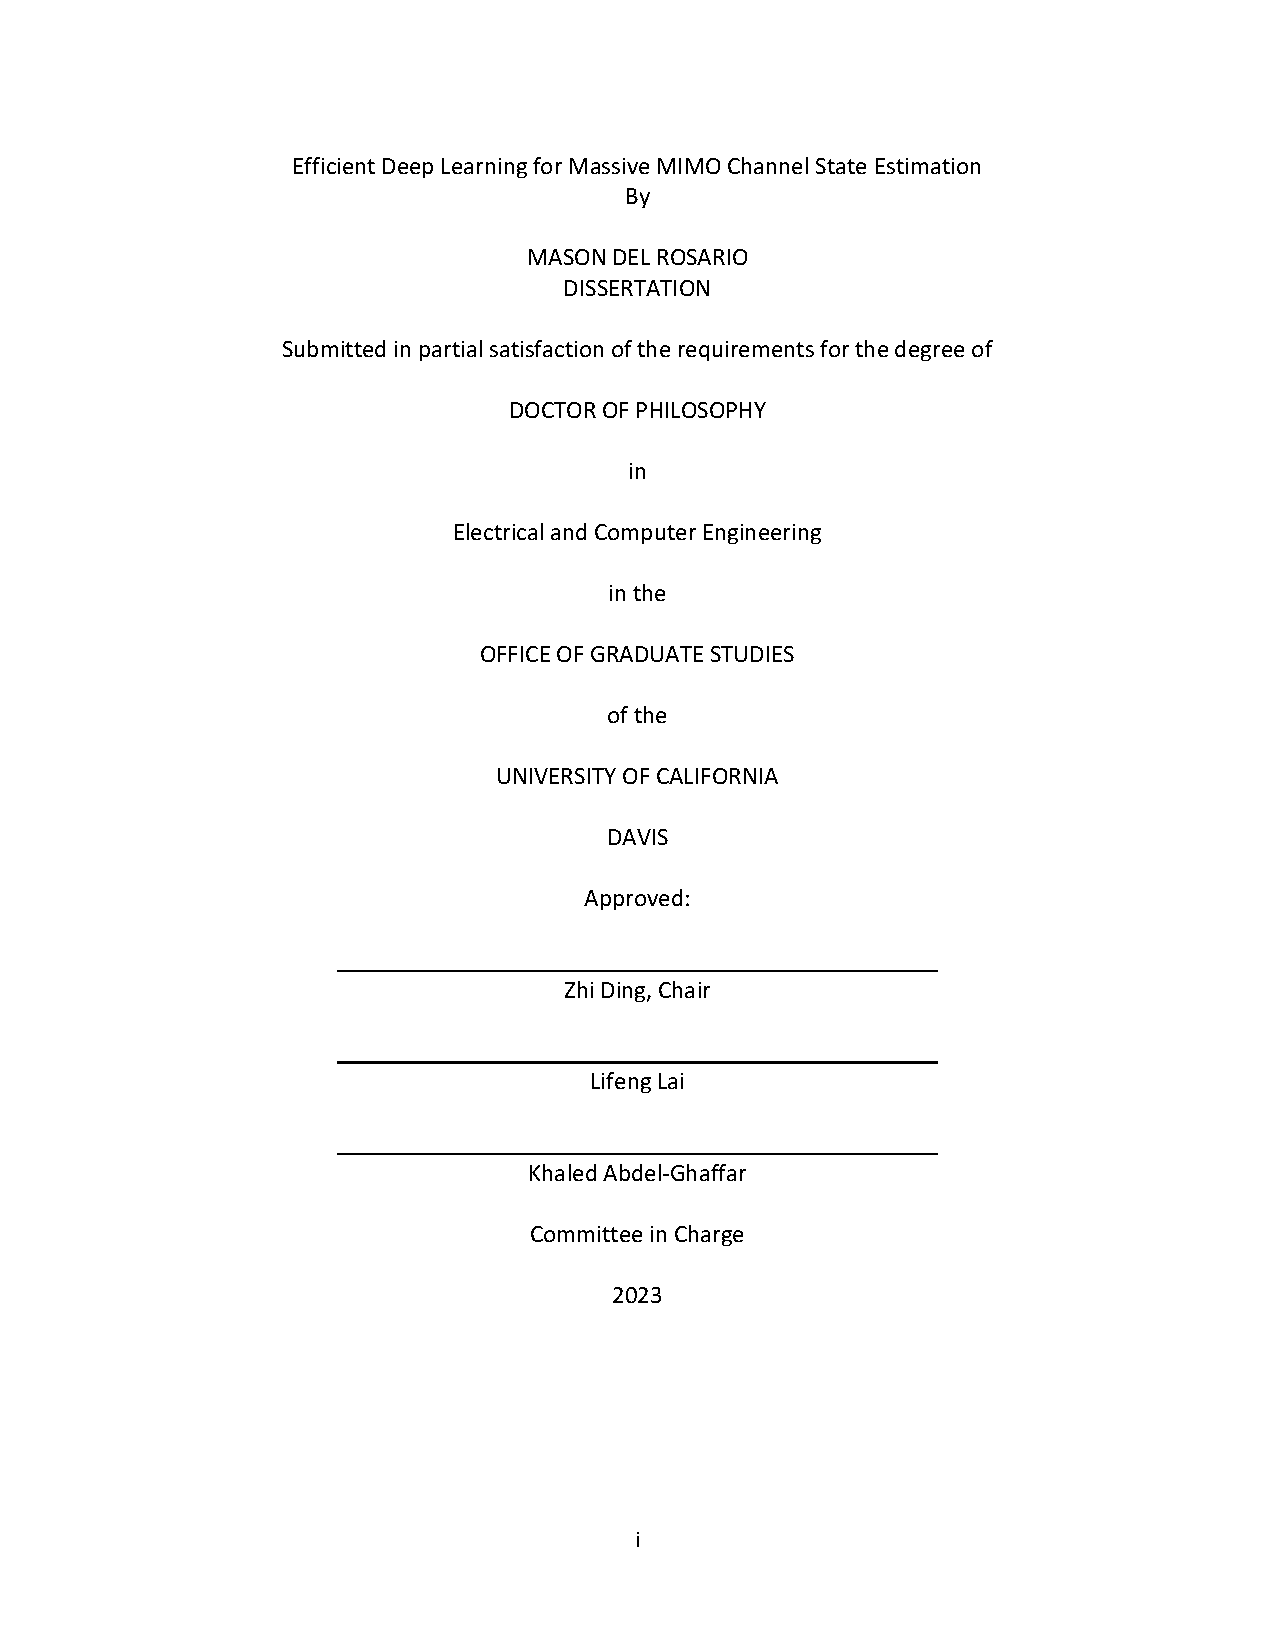
\includepdf{title_page/title_page_mdr.pdf} % include UCD template title page in frontmatter

\pagenumbering{roman}

\stepcounter{page} % increment page number, accounting for title page
\chapter*{Acknowledgements}
% \thispagestyle{empty}

The research conducted in this dissertation was supported by the  National Science Foundation under Grant No. ECCS-1711823, ECCS-2029027, and CNS-2002937.

% \clearpage

\tableofcontents
\listoffigures
\listoftables

\newpage
\pagenumbering{arabic}
\newpage
{\baselineskip 14pt \rightline{Mason del Rosario} \rightline{September,
\the\year} \rightline{Electrical and Computer Engineering}} \vspace{27pt}
\centerline{\Huge \bf {Abstract}} \vspace{18pt}
\addcontentsline{toc}{section}{Abstract}

Future wireless communications networks will rely heavily on massive MIMO technologies where a base station (BS) with large multiantenna arrays serve a large number of user equipment (UE) terminals. Such multiantenna arrays enable high capacity communications via beamforming, as evidenced by work in information theory \cite{ref:goldsmith2003capacity}. To achieve capacity in massive MIMO networks, the base station requires accurate estimates of downlink channel state information (CSI) in order to precode (decode) transmitted (received) messages \cite{ref:marzetta2016fundamentals}.

CSI can be acquired using pilot signals, and in time-division duplex (TDD) mode, channel reciprocity allows the BS to estimate the downlink CSI via pilots in uplink transmissions. However, in frequency division duplex (FDD) mode, channel reciprocity between uplink and downlink channels is weak, and the BS must rely on feedback from the UE to estimate downlink CSI. Specifying an appropriate CSI feedback scheme is a key issue and involves a reducing feedback bandwidth while maintaining accurate downlink CSI estimates.

Conventional methods for CSI feedback compression typically rely on compressed sensing (CS), which seeks to reconstruct high-dimensional data based on low-dimensional measurements (see \cite{ref:Marques2019ReviewOfSparseRecovery} for a survey of CS methods). Many CS methods rely on convex relaxations of an underdetermined least-squares problem, and such methods rely on iterative solvers (e.g., the proximal gradient method). When using an iterative solver, reconstruction can consume an undue amount of time even when measurements are available, making faster methods for reconstruction desirable.

Recent work in deep learning for compressed CSI estimation has presented viable alternatives to CS methods \cite{ref:csinet}. Such work typically employs convolutional neural networks (CNNs) to learn compressed representations of high-dimensional CSI, and the architectures used in CNN-based works can be placed in one of two categories. The first category, CNN-based autoencoders, consists of networks which utilize two subnetworks: an encoder network which learns a low-dimensional representation with the original data as an input and a decoder network which estimates the original data as a function of the low-dimensional representation. The second category, unrolled optimization networks, draws inspiration from the aforementioned CS methods by structuring the CNN as a finite number of repeated blocks with each block imitating an iteration of a given CS algorithm.

This thesis explores both CNN autoencoders and unrolled optimization networks for CSI estimation while focusing on domain knowledge, including physical insight into the wireless channel or features of the communications protocol, to improve the performance of these CSI estimation networks with respect to accuracy, feedback rate, or network efficiency. Prior works have demonstrated superior performance of these architectures over conventional CS methods \cite{ref:csinet,ref:Guo2022FISTANet}, and this thesis investigates the myriad ways that domain knowledge of wireless channels and communications protocols can be leveraged to improve CSI estimation.

% Other points to touch on
% - Accounting for pilots? P2D
% - Bridging gap b/n compressed sensing and deep learning?
%   - Why do autoencoders underperform deep CS methods? Does any lit support this (yes in CV)?
\chapter{Introduction}
\label{chap:intro}

% TODO: updates to make:
% - 1.1 MIMO Channel overview
% 	- Add more discussion about MIMO CSI, capacity, precoding/beamforming, 
%	- Add details about 3GPP specificaions (possibly from latest preprint?)
% - Add more 

% Section \ref{sect:notation} introduces the notation used through this work.
This dissertation details work in improving the accuracy and efficiency of deep learning methods for MIMO channel state information estimation. This chapter provides the necessary background to understand the contributions of the dissertation. Section \ref{sect:mimo_model} provides an overview of the MIMO channel and the importance of CSI estimation in MIMO-based communications networks. Section \ref{sect:channel_model} discusses MIMO channel models and introduces the primary channel model used in this work, the COST2100 model. Section \ref{sect:classic_estimation} discusses prior work in compressed sensing for CSI estimation. Section \ref{sect:dl_overview} provides a generic overview of deep learning. 
Boldface lowercase (uppercase) letters indicate vectors (matrices). Unless otherwise specified, the norm $\|\cdot\|$ indicates the Frobenius norm. Superscripts $^T$ ($^H$) indicate the transpose (Hermitian transpose).
% recent work in deep learning for CSI estimation in MIMO networks

\section{MIMO Channel Overview}
\label{sect:mimo_model}

\begin{figure}[!hbtp]
\centering
{
	\fontsize{6pt}{8pt}
	\def\svgwidth{0.8\columnwidth}
	\input{images/mimo-schematic.pdf_tex}
}
\caption{Example multi-antenna transmitter (BS, gNB) and single-antenna user equipment (UE) and relevant system values.}
\label{fig:mimo_schematic}
\end{figure}

In this work, we consider a MIMO channel with a multiple antennas ($N_B \gg 1$) at the transmitter (gNodeB or gNB) servicing a single user equipment (UE) with a single antenna. Under orthogonal frequency division multiplexing (OFDM) with $N_f$ subcarriers, the received symbols on the $m$-th subcarrier for the downlink and the uplink at the receiver are given as
\begin{align*}
	y_{d,m} &= \mathbf h_{d,m}^H\mathbf w_{t,m}x_{d,m} + n_{d,m}.
	% y_{u,m} &= \mathbf w_{r,m}^H\mathbf h_{u,m}x_{u,m} + \mathbf w_{r,m}^H\mathbf n_{u,m},
\end{align*}
where the individual system values are defined in Table~\ref{tab:mimo-params}, and a representative system model is viewable in Figure~\ref{fig:mimo_schematic}. The resulting downlink and uplink channel state information (CSI) matrices are given as
\begin{align*} 
	\bar{\mathbf H}_d &= \begin{bmatrix} \mathbf h_{d,1} & \dots & \mathbf h_{d,N_f}\end{bmatrix}^H \in \mathbb C^{N_f \times N_b}.
	% \bar{\mathbf H}_u &= \begin{bmatrix} \mathbf h_{u,1} & \dots & \mathbf h_{u,N_f}\end{bmatrix}^H \in \mathbb C^{N_f \times N_b}.
\end{align*}
\begin{table}[]
\renewcommand{\arraystretch}{1.25}
\centering
\caption{MIMO system variables considered in this work.}
\label{tab:mimo-params}
\begin{tabular}{c|c|l}
\toprule
\textbf{Symbol}   	  	  & \textbf{Dimension}            & \textbf{Description} \\ \midrule
$y_{d,m}$ 		  	  	  & $\mathbb{C}^{1}$ 			  & Received downlink symbol on $m$-th subcarrier  \\ \hline
$\mathbf h_{d,m}$ 	  	  & $\mathbb{C}^{N_b \times 1}$   & Downlink channel on $m$-th subcarrier  \\ \hline
$\bar{\mathbf H}_{d}$ 	  & $\mathbb{C}^{N_f \times N_b}$ & Downlink CSI (spatial-frequency domain)  \\ \hline
$\mathbf w_{t,m}$ 	  	  & $\mathbb{C}^{N_b \times 1}$   & Transmitter precoding vector for $m$-th subcarrier  \\ \hline
$x_{d,m}$ 		  	  	  & $\mathbb{C}^{1}$ 			  & Trasmitted symbol on $m$-th subcarrier  \\ \hline
$n_{d,m}$ 		  	  	  & $\mathbb{C}^{1}$ 			  & Downlink noise on $m$-th subcarrier  \\ \hline
$\tilde{\mathbf H}_{d}$   & $\mathbb{C}^{N_f \times N_b}$ & Downlink CSI (angular-delay domain)  \\ \hline
$\mathbf H_{d}$   		  & $\mathbb{C}^{R_d \times N_b}$ & Truncated downlink CSI (angular-delay domain)  \\ \hline
% $y_{u,m}$ 		  & $\mathbb{C}^{1}$ 			  & Received uplink symbol on $m$-th subcarrier  \\ \hline
% $\mathbf h_{u,m}$ & $\mathbb{C}^{N_b \times 1}$   & Uplink channel on $m$-th subcarrier  \\ \hline
% $\mathbf H_{u}$   & $\mathbb{C}^{N_f \times N_b}$ & Downlink impulse response on $m$-th subcarrier  \\ \hline
% $\mathbf w_{r,m}$ & $\mathbb{C}^{N_b \times 1}$   & Received precoding vector for $m$-th subcarrier  \\ \hline
% $x_{u,m}$ 		  & $\mathbb{C}^{1}$ 			  & Received symbol on $m$-th subcarrier  \\ \hline
% $\mathbf n_{u,m}$ & $\mathbb{C}^{1}$ 			  & Uplink noise on $m$-th subcarrier  \\ \hline
\end{tabular}
\end{table}
To achieve near-capacity transmission rates, the transmitter needs access to an appropriate estimate of $\bar{\mathbf H}_d$ \cite{ref:goldsmith2003capacity}. Such estimates enable the use of linear precoding techniques (e.g., conjugate beamforming or zero-forcing beamforming) to realize appreciable spectral and power efficiency gains \cite{ref:yang2013performance}. Downlink CSI estimation can be performed in time division duplex (TDD) by using uplink pilots due to channel reciprocity \cite{ref:Kaltenberger2010relative,ref:mi2017massive,ref:Gao2010utilization}. In contrast, frequency domain duplex (FDD) does not admit channel reciprocity due to frequency-selective channels, meaning CSI estimates must be acquired at the UE using pilot signals, and these estimates must be compressed then fed back to the BS.

\section{Practical Pilot-based Channel Estimation in 4G/5G Networks}
\label{sect:pilots}

% \section{Sparse Pilots in Practical Networks}
To estimate the downlink CSI in wireless networks, transmitters allocate pilot reference signals. To reserve spectral resources, pilots are restricted to a limited number of spatial-frequency positions, and the allocation of these pilots is defined in the 3GPP technical standards, TS 36.211 for 4G/LTE networks \cite{ref:3gpp.36.211} and TS 38.211 for 5G/NR networks \cite{ref:3GPPTS38.211V15.8.0}. In these two standards, the pilots are called CSI reference signals (CSI-RS) or demodulation reference signals (DM-RS), respectively. Figure~\ref{fig:lte-vs-5g} shows valid placements of CSI-RS/DM-RS in the time-frequency resource grid as defined by TS 36.211 and TS 38.211.

\begin{figure}[!hbtp]
    \centering
    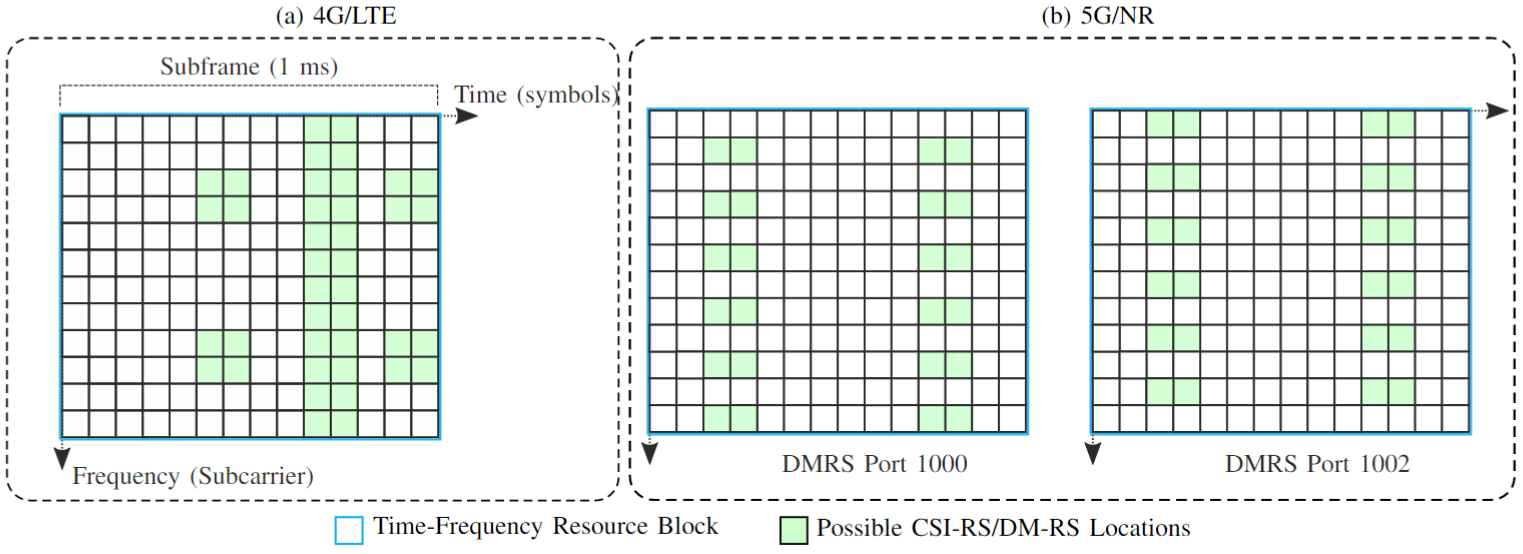
\includegraphics[width=\linewidth]{LTE_vs_5GNR_resource_grid.png}
    \caption{(a) LTE resource blocks with CSI-RS locations. (b) 5G NR resource blocks with DM-RS locations.}
    \label{fig:lte-vs-5g}
\end{figure}

While many using deep learning for CSI estimation do not address pilot estimation explicitly, a few works have incorporated pilot estimation into the CSI feedback problem. 

\section{Geometric Stochastic Channel Models (GSCMs)}
\label{sect:channel_model}

Ideally, the datasets used for the CSI estimation task would be derived from measurement campaigns (e.g., see \cite{ref:shepard2016argoschannel,ref:du2021interuserangle,ref:li20222finegrained}). However, the financial and labor costs of acquiring these datasets can be prohibitive in certain situations. In such situations, researchers rely on  rely on geometric stochastic channel models (GSCMs), models which are so called since they consider the \textbf{geometry} of scatterers in the wireless environment and the \textbf{stochastic} nature of the channel. Simulations based on GSCMs are advantageous to researchers for a a few reasons:
\begin{enumerate}
	\item Simulations permit the generation a large quantities of data in a (relatively) short period of time.
	\item Simulations enable the adjustment of parameters of the communications system (e.g., carrier frequency, UE mobility, subcarrier spacing).
\end{enumerate}

GSCMs consider the problem of modeling the wireless channels at two different scales. At a small-scale, the focus is on th meodeling of ``scatterers,'' objects in the environment which reflect the electromagnetic waves transmitted during. Examples of scatterers in an outdoor environment are buildings, balconies, cars, and trees, while examples of scatters in an indoor environment are walls, furniture, and people. Due to the presence of many scatterers, electromagnetic waves transmitted from a BS arrive at UEs along multiple paths at different delays, and accordingly, the scatterers are often referred to as \textbf{multipath components (MPCs)}. From the UE's perspective, the MPCs are often grouped together in specific delay regions, and each such grouping of MPCs is referred to as a \textbf{cluster}. In GSCMs, modeling is done at a cluster-level, capturing the diverse effects of many MPCs that are present in typical real-world wireless channels. Modeled clusters are typically parameterized by three values: delay, direction of departure (DoD), and direction of arrival (DoA).  

While the modeling of MPCs and clusters is vital, also vital is ensuring that the results of the GSCM-based simulations are statistically consistent with the measured channel data. This consistency is ensured by selecting \textbf{large-scale parameters (LSPs)}, examples of which are the delay spread and the angular spread. In designing GSCMs, the goal is to balance the fidelity of cluster behavior (based on delay, DoD, DoA) and of LSPs when compared to measured channel data. In practice, researchers implement GSCMs based on two different modeling approaches: system-level modeling or cluster-level modeling.

In system-level modeling, the interaction(s) between the BS and the UE(s) is first defined by choosing LSPs. This selection of LSPs is done by sampling from probability distributions. Based on the LSPs, the clusters and MPCs for each BS/UE interaction is defined.

While some well-known channel models, such as the 3GPP Spatial Channel Model (SCM) \cite{ref:kyosti2007winner} and the WINNER II \cite{ref:kyosti2007winner}, adopt the system-level approach, this modeling approach has some salient limitations. First, system-level models do not lend themselves well to high-mobility scenarios, as the LSPs are likely to change as the position of UEs change substantially. Second, system-level models make the addition of new LSPs (e.g., inter-link correlation) to a given interaction.

In contrast with system-level models, cluster-level models begin with cluster/MPC definition then move on to LSPs. First, a large number of clusters are defined by sampling from a chosen probability distribution. Then, the location(s) of UE(s) is (are) defined, and the scattering of each cluster is calculated based on the ``visibility'' of UEs with respect to the clusters. Finally, the LSPs are synthesized by sampling from a given probability distribution.

The cluster-level approach addresses both of the issues associated with system-level approaches. Simulating time-varying channels with high mobility is straightforward since it involves recalculating UE visibility and LSPs, and layering new LSPs into the model is simple since it is the last step of the simulation.

For all CSI tests, we mainly rely on a cluster-level GSCM, the COST2100 channel model,  \cite{ref:liu2012cost2100}. We use two datasets with a single base station (gNB) and a single user equipment (UE) in the following scenarios:
\begin{enumerate}
	\item \textbf{Indoor} channels using a 5.3GHz downlink at
	0.001 m/s UE velocity, served by a
	gNB at center of a $20$m$\times 20$m coverage area.
	\item \textbf{Outdoor} channels using a 300MHz downlink at 0.9 m/s UE velocity served by a gNB at center 
	of a $400$m$\times 400$m coverage area.
\end{enumerate}
In both scenarios, we use the parameters listed in Table~\ref{tab:cost-params}.
\begin{table}[]
\centering
\caption{Parameters used for COST2100 simulations for both Indoor and Outdoor datasets.}
\label{tab:cost-params}
\begin{tabular}{c|c|l}
\toprule
\textbf{Symbol} & \textbf{Value} & \textbf{Description} \\ \midrule
$N_b$ 			& 32			 & Number of antennas at gNB  \\ \hline
$N_f$ 			& 1024			 & Number of subcarriers for OFDM link  \\ \hline
$R_d$ 			& 32			 & Number of delay elements kept after truncation  \\ \hline
$N$ 			& $10^6$		 & Total number of samples per dataset  \\ \hline
$T$ 			& 10		 	 & Number of timeslots  \\ \hline
$\delta$		& 40 ms			 & Feedback delay interval between consecutive CSI timeslots  \\ \bottomrule
\end{tabular}
\end{table}

\section{Classical CSI Estimation}
\label{sect:classic_estimation}

Works in compressive feedback for CSI estimation in MIMO networks can be placed in three broad categories. The first category includes works which use direct quantization of continuous CSI elements to discrete levels. The quantized CSI are encoded and fed back to the transmitter \cite{ref:makki2012hybrid,ref:shirani2009channel}. The second category includes works which use compressed sensing, a technique which applies a random measurement matrix at the transmitter and the receiver \cite{ref:rao2014distributed, ref:eltayeb2014compressive}. Compressed sensing assumes matrices to be encoded and fed back meet certain sparsity requirements, and compressed sensing algorithms require iterative solvers \cite{ref:do2008sparsity} for decoding, resulting in undesired latency.

The last category of work in compressive CSI feedback uses deep learning (DL), neural networks with numerous layers which are trained on large datasets using backpropagation. We will provide the background knowledge needed for deep learning in Chapter 2, Section~\ref{sect:dl_overview}.

\section{Objective and Contributions}

Successful efforts in DL for CSI estimation have typically utilized convolutional neural networks (CNNs) in an autoencoder structure \cite{ref:csinet}. Variations on the CNN-based autoencoder have investigated different network architectures \cite{ref:Lu2020CRNet}, variational training frameworks \cite{ref:Hussien2020PRVNet}, and denoising modules \cite{ref:Sun2020AnciNet}. These architectural changes are largely inspired by successful application of DL in image compression \cite{ref:szegedy2017inception,ref:balle2017end,ref:xie2012image}.

While they can continue to push the state-of-the-art in CSI reconstruction accuracy, architectural optimizations may ultimately follow the same trends of fields such as language modeling, where state-of-the-art performance requires prohibitively massive compute \cite{ref:brown2020language}. In this proposal, we take a different approach seek to improving compressive channel feedback by focusing on domain knowledge and physical insight.
% While the powerful functional approximation of deep CNNs has enabled state-of-the-art CSI reconstruction accuracy, they run the risk falling into the same trap as the image.

This thesis details our attempts to use domain knowledge to enhance the performance and the efficiency of neural networks for CSI estimation (for a visual summary, see Figure~\ref{fig:contrib}). Section~\ref{chap:sph_norm} details our work in power-based normalization, which leverages CSI sparsity. Section ~\ref{chap:markovnet} describes our work in differential encoding, which exploits temporal coherence of CSI. Section~\ref{chap:p2d} describes our work in pilot-based delay domain CSI estimation.

\begin{figure}[htb] \centering 
	{
	  \fontsize{4pt}{4pt}
	  \def\svgwidth{0.9\columnwidth}
	  % \input{images/cnns-venn-diagram-contrib.pdf_tex}
	}
	\caption{Venn diagram highlighting different aspects of domain knowledge in CNN-based CSI compressive feedback, relevant convolutional networks, and our contributions.}
	\label{fig:contrib}
\end{figure}
\chapter{Deep Learning for CSI Estimation}
\label{chap:sph_norm}

In this chapter, we will discuss important aspects of successfully applying deep learning to MIMO CSI estimation. In Section~\ref{sect:dl_overview}, we provide a basic overview of deep learning concepts that are pertinent to the task of CSI estimation. In Section~\ref{sec:data-preprocessing}, we discuss data pre-processing techniques and the applications of domain knowledge that have enabled deep learning-based CSI estimation. In Section~\ref{sect:sph_norm}, we describe our proposed CSI pre-processing technique, spherical normalization, which boosts estimation accuracy without significantly changing the computational complexity of a given estimation algorithm. 

\section{Deep Learning Background}
\label{sect:dl_overview}

This section provides a brief overview of relevant deep learning concepts employed in this work, including convolutional neural networks (CNNs), autoencoders, and unsupervised learning.

\textbf{Deep learning (DL)} is a subset of machine learning (ML), a broad class of algorithms which use data to ``fit'' models for prediction or classification tasks. The three predominant learning frameworks are supervised learning, unsupervised learning, and reinforcement learning. In the works proposed, we focus on \emph{unsupervised learning}, which seeks to find a compressed representation of the data without labels (see Chapter 14 of \cite{ref:Hastie2016Elements} for an overview).

\textbf{Convolutional Neural Networks (CNNs)}: A neural network is a machine learning algorithm with multiple \emph{layers} of parameterized linear functions followed nonlinear functions (typically referred to as `activation' functions). The parameters for these layers can be updated via a stochastic optimizer (e.g., the Adam optimizer \cite{ref:Kingma2014ADAM}), and given enough layers, such networks can achieve arbitrarily accurate functional approximation \cite{ref:Hecht1992TheoryBackprop}. In recent years, neural networks with convolutional layers have established state-of-the-art performance in computer vision tasks such as image classification \cite{ref:Sabour2017Dynamic} and segmentation \cite{ref:He2017Mask}. While the concept of a CNN has been around since at least the early 80's \cite{ref:fukushima1980neocognitron}, CNNs did not see widespread adoption in computer vision until AlexNet \cite{ref:krizhevsky2012imagenet}. This recent proliferation of CNNs in computer vision has been enabled by hardware advances  such as graphical processing units (GPUs) and tensor processing units (TPUs) which make parallel training on large-scale datasets possible.

\begin{figure}[!hbtp]
\centering
\def\svgwidth{0.8\columnwidth}
\input{images/autoencoder_schematic.pdf_tex}
\caption{Abstract schematic for an autoencoder operating on CSI matrices $\mathbf H$. The encoder learns a latent representation, $\mathbf Z$, while the decoder learns to reconstruct estimates $\hat{\mathbf H}$.}
\label{fig:autoencoder_schematic}
\end{figure}

A common architecture for deep unsupervised learning is the \emph{autoencoder} (see Fig.~\ref{fig:autoencoder_schematic} for a generic example). Trained end-to-end on input data, an autoencoder is comprised of an encoder and a decoder which jointly learn a compressed latent representation ($\mathbf Z$) and an estimate of the input ($\hat{\mathbf H}$). By choosing $\mathbf Z$ to have lower dimension than the input, the network is forced to learn a ``useful'' summary of the input data. The typical objective function for such a network is the mean squared error (MSE),
\begin{align*}
\underset{\theta_e, \theta_d}{\text{argmin}}\; \frac 1N \sum_{i=1}^N\Arrowvert \mathbf H_i - g(f(\mathbf H_i, \vec\theta_e), \vec\theta_d) \Arrowvert^2.
\end{align*}
We optimize network parameters $\vec \theta_e, \vec \theta_d$ by backpropagation and a stochastic optimization algorithm (e.g., stochastic gradient descent or Adam).

The first CNN autoencoder used for the CSI estimation task was CsiNet \cite{ref:csinet}. Figure~\ref{fig:csinet} shows the architecture of CsiNet, where the encoder is deployed at the UE and the decoder is deployed at the BS. The encoder uses a convolutional layer and a linear layer to find a compressed representation of the input CSI, and the decoder uses a linear layer to expand the dimension of the feedback followed by two ``refine blocks'' and an output convolutional layer to refine the CSI estimate. After the CsiNet paper, many works attempted to bolster the performance of CNN autoencoders for CSI estimation by incorporating \emph{domain knowledge}. This chapter details several such works, and in Section \ref{sect:sparse-csi}, we will discuss one such area of domain knowledge about CSI data: the sparse basis of the CSI data utilized in CsiNet. 

\begin{figure}[htb]
	\centering
	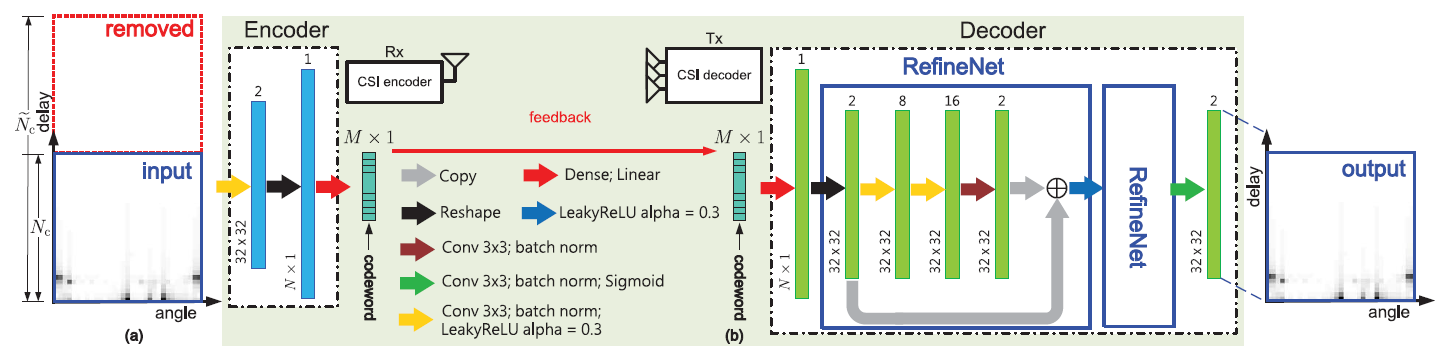
\includegraphics[width=\textwidth]{csinet-fig-paper.png}
	\caption{CsiNet architecture from \cite{ref:csinet}}
	\label{fig:csinet}
\end{figure}

\textbf{Computational Complexity}: Given the number of layers and operations involved in any deep learning algorithm, measuring the \textbf{computational complexity} of these algorithms is important. Two metrics that are commonly used in deep learning literature are:

\begin{enumerate}
	\item \textbf{Floating point operations (FLOPs)}: FLOPs provide a measure of the computations used by a given layer or mathematical operation in a network. A single FLOP is defined as any arithmetic operation between floating point numbers (e.g., addition, multiplication) or any assignment of a floating point value.
	\item \textbf{Parameters}: The number of parameters in a deep learning network determines the storage cost for inference\footnote{The size of the dataset will contribute towards the storage cost but only during training/evaluation.}. The number of parameters in a typical deep learning model can be anywhere from millions (e.g., ResNet architectures \cite{ref:he2016identity}) to billions (e.g., GPT-3 \cite{ref:brown2020language}).
\end{enumerate}

See Appendix~\ref{appdx:complexity} for a more exhaustive discussion of common layers/operations used in deep networks and their corresponding computational complexity.

% For data with multiple input features of different scales. In ML curricula, this is often illustrated using the iris dataset \cite{ref:anderson1936species,ref:fisher1936use}), which contains .

\section{Data Pre-processing for CSI Data} \label{sec:data-preprocessing}

The success of machine learning tasks relies on proper \emph{data pre-processing}, a sequence of transformations used on the input data before fitting a model. In any machine learning task, data pre-processing is necessary to ensure that the scales of input features are similar. In deep learning for CSI estimation, three important pre-processing techniques are domain transformations, truncation, or normalization, and in this section, we will explore the important choices in pre-processing that authors have made based on domain knowledge of MIMO CSI data.

\subsection{Sparse Basis for CSI} \label{sect:sparse-csi}

\begin{figure}[htb]
	\centering
	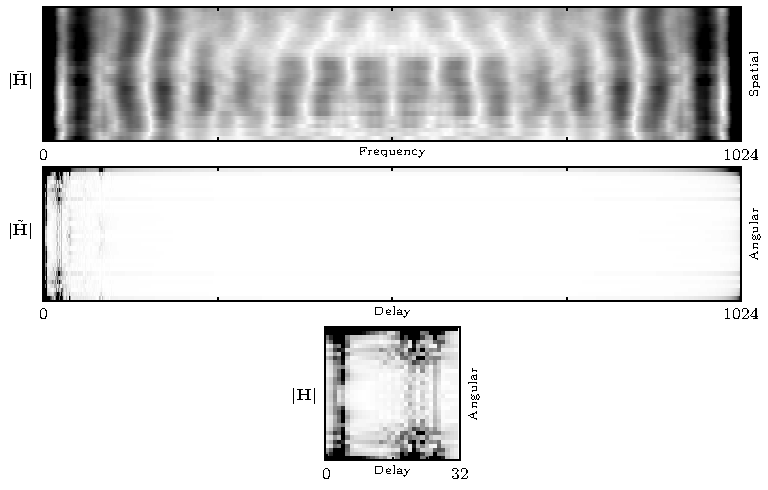
\includegraphics[width=.8\textwidth]{batch17_sample0_freqvsdel_truncatevsfull.pdf}
	\medskip
	\caption{Magnitude of spatial-frequency ($\bar{\mathbf H}$), angular-delay ($\tilde{\mathbf H}$), and truncated angular-delay ($\mathbf H$) representations for a single random channel from the outdoor COST2100 dataset.}
	\label{fig:freq-vs-delay}
\end{figure}

The first type of data pre-processing we consider is a domain transformation, the discrete Fourier transform in particular. While the \textbf{spatial-frequency} representation $\bar{\mathbf H}$ is used for beamforming at the transmitter, the number of non-zero elements is comparatively large. Given the dimension of $\bar{\mathbf H}$, feeding back entire CSI matrices is impractical. Instead, we seek a compressed representation of a sparse transformation. The sparse representation we consider is the angular-delay representation of CSI matrices \cite{ref:sayeed2002deconstructing}. Denote the unitary inverse DFT for the spatial (frequency) axis as $\mathbf F_a \in \mathbb C^{N_b \times N_b}$ ($\mathbf F_d^H \in \mathbb C^{N_f \times N_f}$), and denote the spatial-frequency CSI matrix as $\bar{\mathbf H}$. The angular-delay domain representation $\tilde{\mathbf H}$ is given as % $\mathbf F \in \mathbb C^{(n_f \times n_f)}$ ($\mathbf F^H \in \mathbb C^{(n_f \times n_f)}$)
\begin{align*}
	\tilde{\mathbf H} &= \mathbf F_d^H \bar{\mathbf H} \mathbf F_a.
\end{align*}
The delay spread of the resulting $\tilde{\mathbf H}$ can typically be captured with a small number of delay elements (see Figure~\ref{fig:outdoor_energy_cdf}), so we restrict our attention to the first $R_d$ elements of $\tilde{\mathbf H}$, resulting in a truncated angular-delay matrix which we denote as $\mathbf H \in \mathbb C^{(R_d\times N_b)}$ for the downlink channel state. An illustrative example of this truncation can be seen at the bottom of Figure~\ref{fig:freq-vs-delay}. % (uplink) ($\mathbf H_u \in \mathbb C^{(R_d\times N_b)}$) 

\begin{figure}[!hbtp]
    \centering
    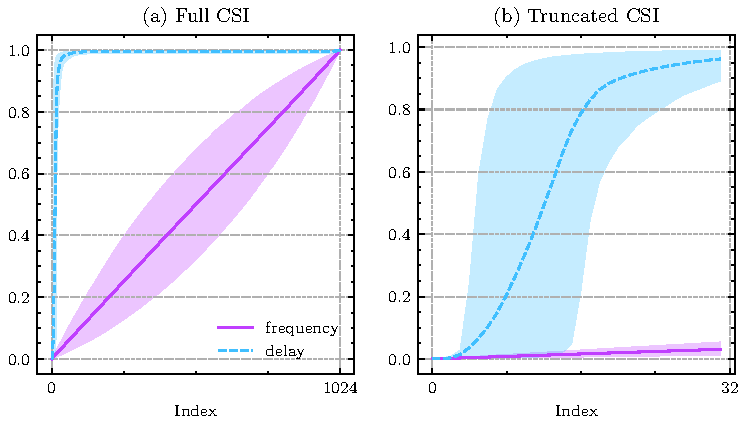
\includegraphics{trunc_energy_cdf_horiz.pdf}
    \caption{Energy CDF for 5000 
    CSI samples
of 32 antennas and 1024 subcarriers, generated
  from 
COST2100 outdoor models described in Section \ref{sect:channel_model}.
Mean percentage of energy in CSI matrix up to index is shown with 90\% confidence intervals. The index denotes the amount of energy accounted for up to the corresponding frequency/delay element. The truncated angular-delay CSI contains a mean energy of 96.2\% (c.i. 89.2\%, 99.1\%), while the truncated frequency-spatial CSI only contains a mean energy of 3.1\% (c.i. 1.2\%, 5.4\%).} 
    \label{fig:outdoor_energy_cdf}
\end{figure}

% Rather than learning a lower dimensional representation of $\bar{\mathbf H}$, the authors of \cite{ref:csinet} chose to compress the \textbf{angular-delay} domain representation of CSI, $\tilde{\mathbf H}$. Given the sparsity of the angular-delay matrices, many works using this basis choose to compress and feedback a truncated version of the CSI matrices, $\mathbf H \in \mathbb R^{R_d \times N_b}$. An illustrative example of this truncation can be seen at the bottom of Figure~\ref{fig:freq-vs-delay}.

\subsection{Bidirectional Reciprocity in FDD Networks}

The next type of pre-processing under consideration is a change of coordinates. Specifically, rather than utilizing a Cartesian representation (i.e., real-imaginary channels), we can consider a polar representation (i.e., magnitude-phase). As discussed in Section~\ref{sect:mimo_model}, the reciprocity of downlink and uplink channels is weak in FDD wireless networks when compared to TDD. Despite this, DL CSI estimation techniques have used uplink CSI to improve the reconstruction accuracy of downlink CSI at gNB. In \cite{ref:dualnet}, the authors demonstrate that the correlation between the magnitude of uplink and downlink CSI elements is strong. To exploit magnitude reciprocity, they propose DualNet, a CNN autoencoder which learns a feedback encoding for the downlink CSI magnitude and decodes the feedback with the magnitude of uplink CSI as side information. The downlink phase is separately quantized and fed back to gNB via magnitude-dependent phase quantization (MDPQ). The authors demonstrate that exploiting bidirectional reciprocity can substantially improve CSI estimation accuracy.

\subsection{Minmax Data Normalization}

The last pre-processing technique we discuss is normalization. Typical deep autoencoders require normalized data to ensure that the range of the input data matches the range of the autoencoder's output function, which is typically chosen as \texttt{sigmoid} or \texttt{tanh} as pictured in Figure~\ref{fig:ae_output_fx}. 
\begin{figure}[htb]
  \centering
  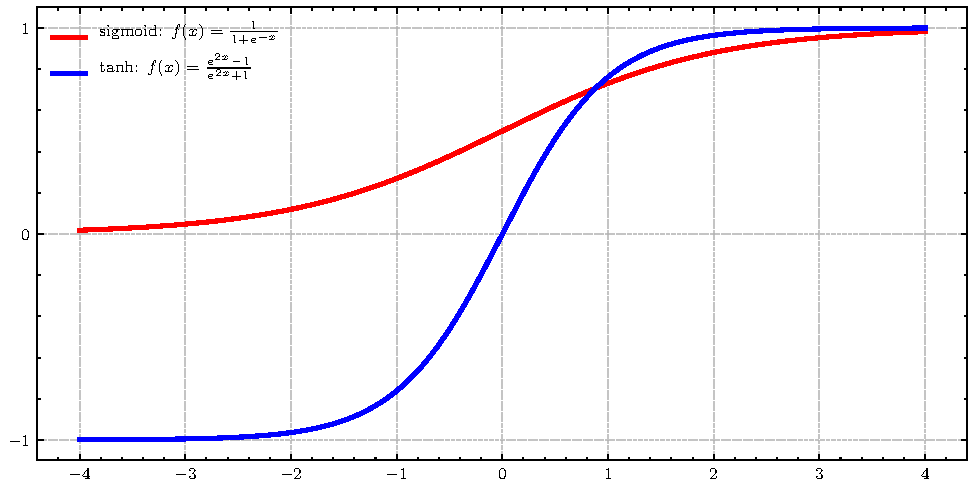
\includegraphics[width=.9\textwidth]{activations.pdf}
  % \medskip
  \caption{Typical activation functions used at the output of convolutional autoencoders.}
  \label{fig:ae_output_fx}
\end{figure}
To accommodate such output functions, most works in both image compression and CSI estimation typically apply \emph{minmax normalization}, where the extrema (i.e., the minimum and the maximum) of the real and imaginary channels are used to scale the entire dataset. For the scalar $H_n(i,j)$, the minmax-scaled version of this element is
\begin{align*}
	H_{n,\text{minmax}}(i,j) &= \frac{H_n(i,j)-H_{\text{min}}}{H_{\text{max}}-H_{\text{min}}} \in [0,1],
\end{align*}
for $n \in [1,\dots,N]$ given a dataset of $N$ samples and $i/j$ indexing the rows/columns of the CSI matrices. The resulting samples are cast to the range $[0,1]$. % Most work in deep learning for CSI estimation focuses on different neural network architectures, training frameworks, or hyperparameter tuning. Such works treat the real and imaginary elements of $\mathbf H$ as separate channels similar to color channels in images.

For image data, minmax normalization results in each image's color channels scaled to the range $[0,1]$. The resulting distribution for each color channel is typically satisfactory for image tasks, as the variance is not much smaller than the range of the normalized data (see Fig.~\ref{fig:imagenet_dist}).

However, for CSI matrices, minmax normalization is applied to the real and imaginary channels of each element. For typical channel models and parameters, the distribution of channel elements tends to have much lower variance than that of image data (see Fig.~\ref{fig:cost_indoor_dist}). This smaller variance can be explained by the difference in the datasets' ranges -- while the channels in image data (e.g., ImageNet) assume integer values between $[0,255]$, the channels in CSI data (e.g., COST2100) assume floating point values smaller than $10^{-3}$.

\begin{figure}[htb]
	\centering
	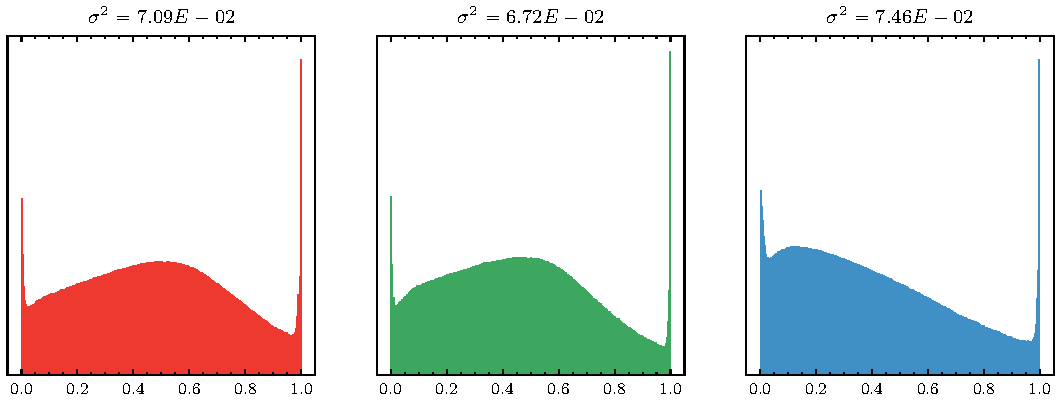
\includegraphics[width=.9\textwidth]{imagenet_rgb_dist.pdf}
	\medskip
	\caption{Distribution and variance of minmax-normalized ImageNet color channels ($N=50000$) images.}
	\label{fig:imagenet_dist}
\end{figure}

\begin{figure}[htb]
	\centering
	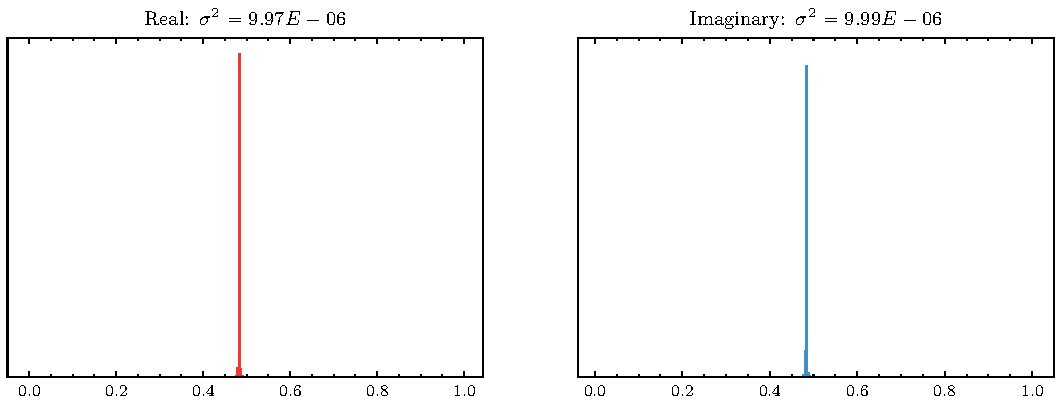
\includegraphics[width=.9\textwidth]{cost2100_indoor_dist.pdf}
	\medskip
	\caption{Distribution and variance of minmax-normalized COST2100 real/imaginary channels ($N=99000$) images.}
	\label{fig:cost_indoor_dist}
\end{figure}

In Section~\ref{sect:sph_norm}, we  will detail our proposed method for increasing the variance of CSI data and demonstrate that this method can improve the estimation accuracy of deep learning networks for CSI estimation.

\subsection{Related Works}

In image processing, several works have investigated normalization techniques such as batch normalization \cite{ref:ioffe2015batch}, instance normalization \cite{ref:huang2017instance}, layer normalization \cite{ref:ba2016layer}, and group normalization \cite{ref:wu2018group}. These normalization techniques scale the outputs of latent layers in neural networks, which helps to solve the problem of covariate shift \cite{ref:ioffe2015batch} where the mean and variance changes between subsequent layers of the network.

Other works have studied normalization of the network's inputs. A number of works have investigated adaptive normalization techniques for time series estimation tasks \cite{ref:ogasawara2010adaptive, ref:nayak2014impact, ref:shao2015self}. In \cite{ref:passalis2019dain}, the authors proposed a trainable input network which learns to shift, scale, and filter the unnormalized data while training the target network for a time series prediction task.

\section{Spherical Normalization} \label{sect:sph_norm}

Here, we discuss our work in spherical normalization (Section~\ref{sect:sph_norm_method}) and our optimized network architecture, CsiNet-Pro (Section~\ref{sect:csinet_pro}) \cite{ref:liu2020sphnet}.

% \subsection{Spherical Normalization}
\label{sect:sph_norm_method}
Rather than apply minmax normalization, which results in a low variance distribution when applied to highly sparse CSI data, we propose spherical normalization. Before describing spherical normalization in detail, consider z-score normalization. Given a random variable, $x$, with mean $\mu$ and standard deviation $\sigma$. The z-score normalized version of this random variable is given as
\begin{align}
	z &= \frac{x - \mu}{\sigma}. \label{eq:zscore}
\end{align}
Assuming $x$ is normally distributed, the resulting random variable, $z$, is a standard normal distribution such that $z \sim \mathcal N(0,1)$. Inspired by $z$-score normalization, we seek a normalization scheme which adjusts the range of each channel sample. Under spherical normalization, each sample in the dataset is scaled by its power. Denote the $n$-th downlink CSI matrix of the dataset as $\mathbf H_d^n$. The spherically normalized version of the downlink CSI is given as
% TODO: Does this make sense? "For CSI matrices, we could choose to scale each element by it's mean and by the inverse covariance matrix."
\begin{align}
	\mathbf{\check H}_d^n &= \frac{\mathbf H_d^n}{\|\mathbf H_d^n\|}. \label{eq:sph-intro}
\end{align}
Observe that (\ref{eq:sph-intro}) is similar to (\ref{eq:zscore}) without the mean shift in the numerator\footnote{Since the mean of COST2100 data is $\approx 10^{-10}$, we can safely ignore this mean shift in spherical normalization.} and with the power term of each CSI sample rather than the variance of the entire distribution. After applying (\ref{eq:sph-intro}) to each sample, minmax scaling is applied to the entire dataset. The resulting dataset under spherical normalization can exhibit a larger variance than the same dataset under minmax scaling (compare Fig.~\ref{fig:cost_indoor_sph_dist} with Fig.~\ref{fig:cost_indoor_dist}). 
\begin{figure}[htb]
	\centering
	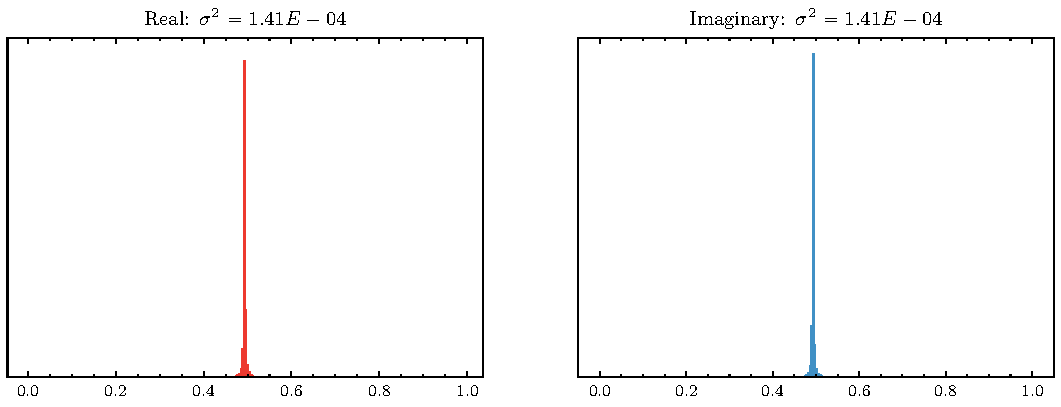
\includegraphics[width=.9\textwidth]{cost2100_indoor_sph_dist.pdf}
	\medskip
	\caption{Distribution and variance of COST2100 real/imaginary channels under spherical normalization ($N=99000$) images.}
	\label{fig:cost_indoor_sph_dist}
\end{figure}

Beyond desirable properties in the input distribution, spherical normalization also results in an objective function which is better matched with the evaluation criterion. Neural networks for CSI estimation are optimized using the mean-squared error loss,
\begin{align} 
	\text{MSE}&=\frac 1N \sum_{k=1}^N\Arrowvert\mathbf H_k - \hat{\mathbf H}_k\Arrowvert^2, \label{eq:mse}
\end{align}
while channel state reconstruction accuracy is measured in terms of normalized mean-squared error,
\begin{align} 
	\text{NMSE}&=\frac 1N \sum_{k=1}^N\frac{\Arrowvert\mathbf H_k - \hat{\mathbf H}_k\Arrowvert^2}{\Arrowvert\mathbf H_k\Arrowvert^2}. \label{eq:nmse}
\end{align}
Observe that when the $\mathbf H_k \; (\hat{\mathbf H}_k)$ in (\ref{eq:mse}) is replaced with $\check{\mathbf H}_k \; (\hat{\check{\mathbf H}}_k)$, we have
\begin{align*} 
	\frac 1N \sum_{k=1}^N\Arrowvert\check{\mathbf H}_k - \hat{\check{\mathbf H}}_k\Arrowvert^2&= \frac 1N \sum_{k=1}^N\left\Arrowvert \frac{\mathbf H_k}{\Arrowvert\mathbf H_k\Arrowvert^2} - \frac{\hat{\mathbf H}_k}{\Arrowvert\mathbf H_k\Arrowvert^2}\right\Arrowvert^2 \\
	&= \frac 1N \sum_{k=1}^N\frac{\Arrowvert\mathbf H_k - \hat{\mathbf H}_k\Arrowvert^2}{\Arrowvert\mathbf H_k\Arrowvert^2},
\end{align*}
which is equivalent to (\ref{eq:nmse}). Thus, a neural network optimized with MSE as the loss function and trained using spherically normalized data is in fact being optimized with respect to NMSE of the original data.

\subsection{CsiNet-Pro}
\label{sect:csinet_pro}

In \cite{ref:liu2020sphnet}, we proposed a network with larger convolutional kernels and no residual connections called CsiNet-Pro. Large kernels (e.g., $(7\times 7)$ in CsiNet-Pro) allow the network to capture features corresponding to larger delay spreads than comparatively small kernels (e.g., $(3\times 3)$ in CsiNet \cite{ref:csinet}). In addition to the compressed feedback of the autoencoder, the encoder must feedback the power of the CSI matrix, $\|\mathbf{H}\|$, meaning the number of floating point elements to feed back increases from $r$ to $r+1$. This can be seen in Figure~\ref{fig:sphnet-arch}, which shows the CsiNet-Pro architecture using spherical normalization, which we refer to as `SphNet.'  
\begin{figure}[htb]
  \centering
  {
    \fontsize{6pt}{6pt}
    \def\svgwidth{1.0\columnwidth}
    \input{images/csinet-pro.pdf_tex}
  }
  % 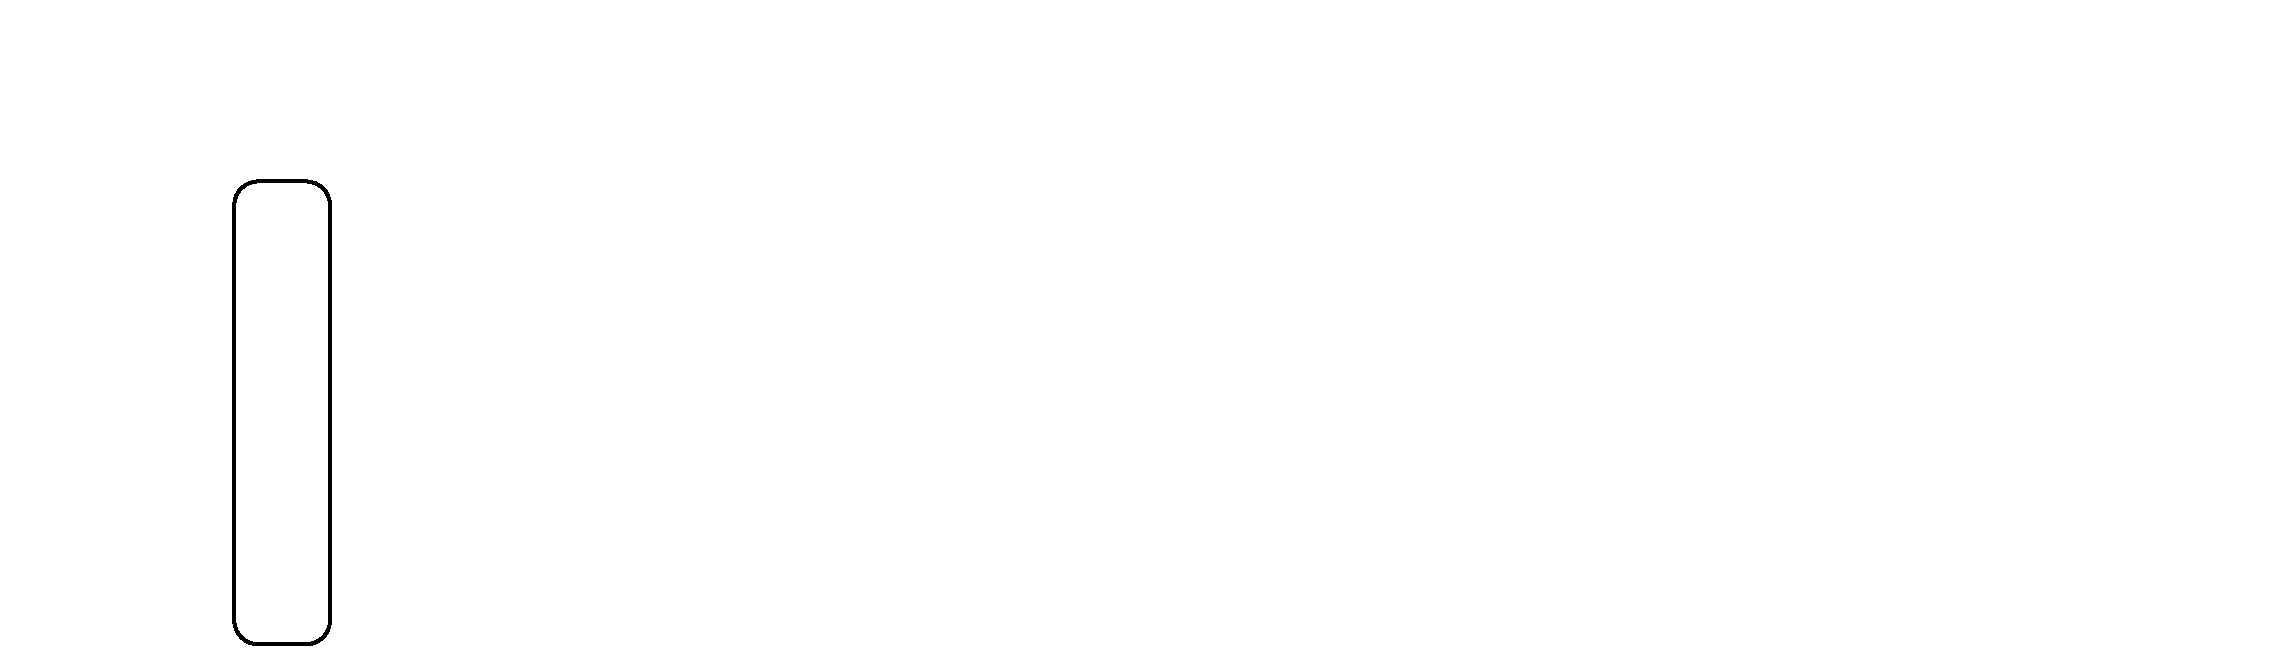
\includegraphics[width=.9\textwidth]{csinet-pro.pdf}
  % \medskip
  \caption{SphNet -- CsiNet-Pro architecture with Spherical Normalization.}
  \label{fig:sphnet-arch}
\end{figure}

\subsection{Results}
Training on spherically normalized data and optimizing with respect to NMSE can yield better accuracy. Fig.~\ref{fig:nmse_slot1} demonstrates this improvement for CsiNet and CsiNet-Pro on the COST2100 dataset. CsiNet and CsiNet-Pro are trained with minmax normalization while CsiNet-Sph and SphNet are trained with spherical normalization. % For both networks, the number of 

\begin{figure}[!hbtp] \centering 
	\begin{subfigure}[t]{.45\textwidth}
		\centering
		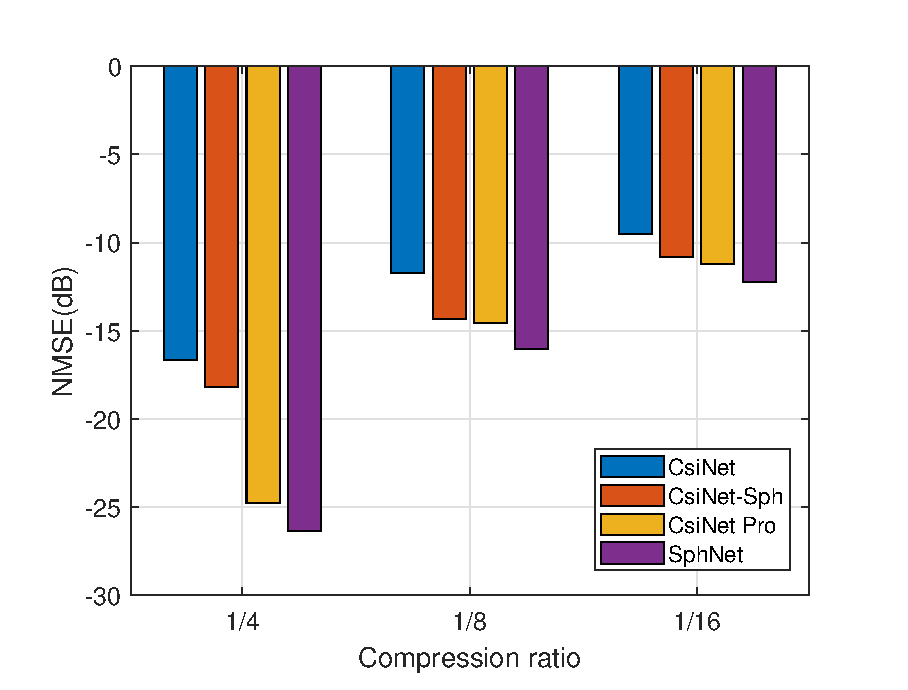
\includegraphics[width=\linewidth]{nmse_slot1_indoor.eps}
		\caption{Indoor}
		\label{fig:slot1_indoor} 
	\end{subfigure}
	\begin{subfigure}[t]{.45\textwidth}
		\centering
		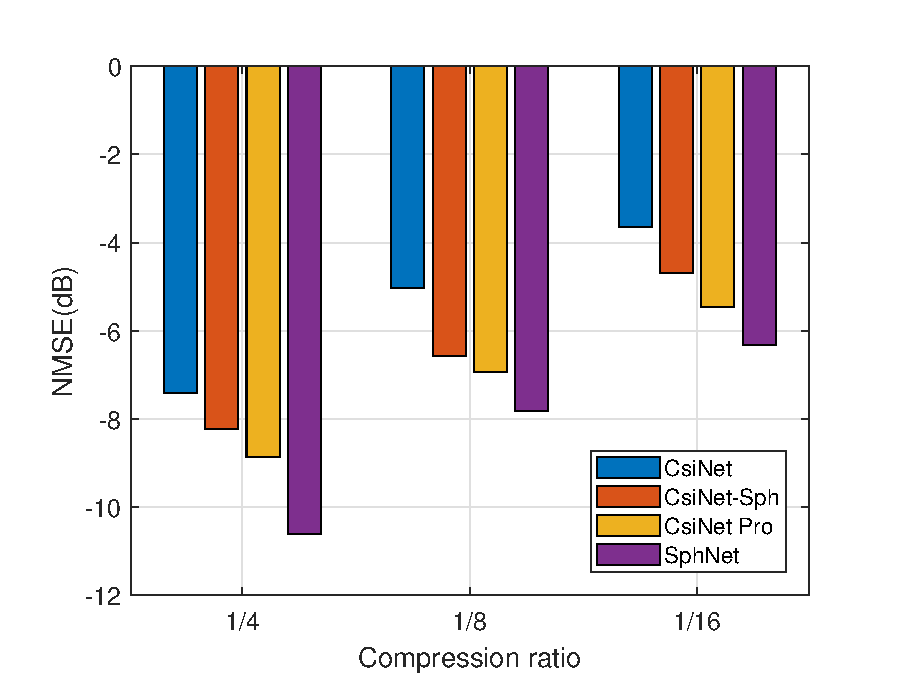
\includegraphics[width=\linewidth]{nmse_slot1_outdoor.eps}
		\caption{Outdoor}
		\label{fig:slot1_outdoor} 
	\end{subfigure}
	\caption{Reconstruction error for CsiNet \cite{ref:csinet} and CsiNet-Pro with and without spherical normalization. SphNet combines CsiNet-Pro with spherical normalization \cite{ref:liu2020sphnet}.}
	\label{fig:nmse_slot1} 
\end{figure}

This chapter has demonstrated the importance of considering unique features of CSI data when applying deep learning to compressive CSI estimation. Making such considerations allowed us to improve estimation accuracy without altering the network's architecture. In the following chapter, we will again consider a unique characteristic of CSI data, temporal correlation of consecutive CSI samples, and we will exploit this correlation to reduce the computational complexity of CSI estimation networks.
\chapter{Temporal Coherence and Differential Encoding}
\label{chap:markovnet}

In this chapter, we consider methods for exploiting temporal correlation between CSI of subsequent timeslots. The \emph{coherence time} of a channel is the amount of time that a channel estimate can be used before that estimate's SNR falls beneath a given threshold \cite{ref:Chopra2016ChannelAging}. Within this window of time ($\Delta t = t_i - t_{i-1}$), the correlation between CSI matrices $\mathbf H_{i}$ and $\mathbf H_{i-1}$ is high (see Figure~\ref{fig:csi_img_gt} for an illustrative example). 
% Works exploiting temporal coherence use CSI matrices from previous timeslots to supplement subsequent estimates \cite{ref:Wang2019CsiNetLSTM}.

\begin{figure}[htb] \centering 
  % 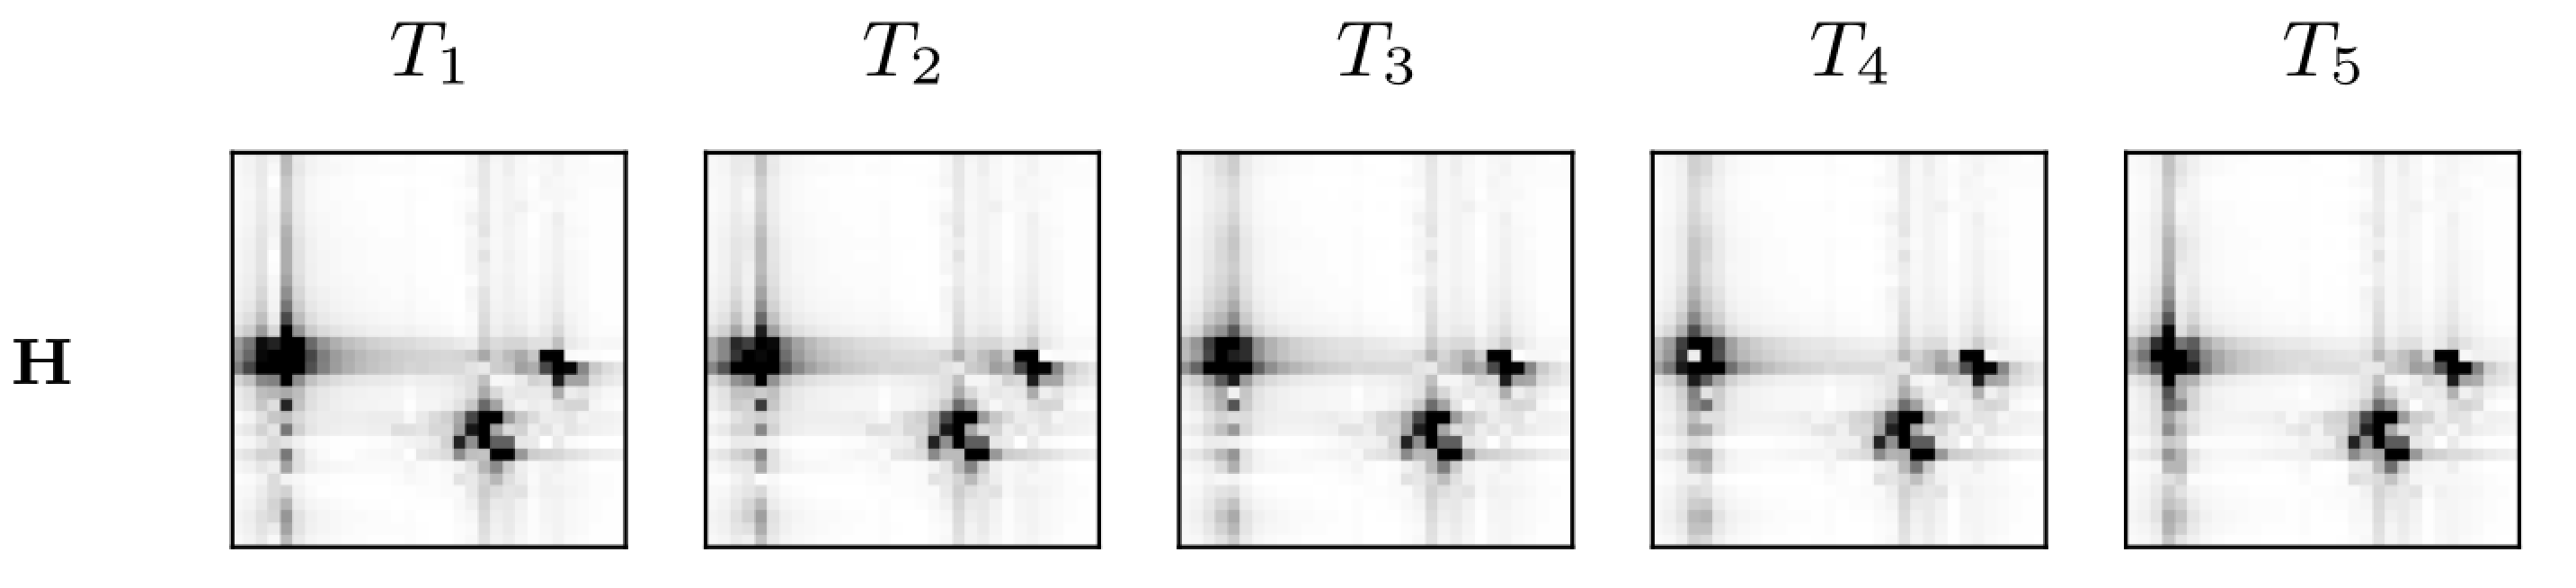
\includegraphics[width=0.9\linewidth]{batch0_csi_gt.png}
{
  \fontsize{10pt}{12pt}
  \def\svgwidth{1.0\columnwidth}
  \input{images/batch0_csi_gt.pdf_tex}
}
  \caption{Ground truth CSI ($\mathbf H$) for five timeslots ($t_1$ through $t_5$) on one sample from the validation set of the outdoor dataset.} 
  \label{fig:csi_img_gt} 
\end{figure}

% Other works in channel state estimation exploit temporal coherence.

Assuming the channel exhibits temporal coherence within a certain window of time,
a reasonably accurate CSI estimate at time $t_{i-1}$ can be used to estimate the CSI at time $t_i$.
Generically, we can write this estimator as
\begin{align}
\grave{\mathbf H}_i &= h(\hat{\mathbf H}_{i-1}) \label{eq:gen_estim}
\end{align}
where $\mathbf{H}_i$ is the CSI matrix at time $t_i$ and $\hat{\mathbf H}_i$ is its estimator. 
The estimation error under $\grave{\mathbf H}_i$ is
\begin{align}
\mathbf E_{i} &= \mathbf H_{i} - \grave{\mathbf H}_{i}. \label{eq:diff_err}
\end{align}

\section{Recurrent Neural Networks}

Prior work in temporal correlation for CSI estimation utilized state-space methods such as the Kalman filter \cite{ref:Huber2006improved,ref:Ali2020BayesKalmanFilter,ref:Kim2021KalmanVsML}. Since it relies on explicit state space and noise models, the Kalman filter's predictive power in CSI estimation is limited. Furthermore, such work generally does not propose a method for feedback compression, making comparison with the following ML methods difficult.

Recent works have leveraged recurrent neural networks (RNNs) to exploit temporal correlation for CSI estimation \cite{ref:Lu2019RecCsiNet, ref:Liao2019BiLSTM, ref:Li2020SpatTempLSTM,
 ref:Jang2019Delay,ref:Wang2019CsiNetLSTM}. RNNs include recurrent layers, such as the long short-term memory (LSTM) cell or the gated recurrent unit (GRU), which are capable of learning long-term dependencies of a given process through backpropagation \cite{ref:Hermans2013Training} and can be used to predict future states of the process \cite{ref:Pascanu2014HowTo}.

\begin{figure}[htb]
	\centering
	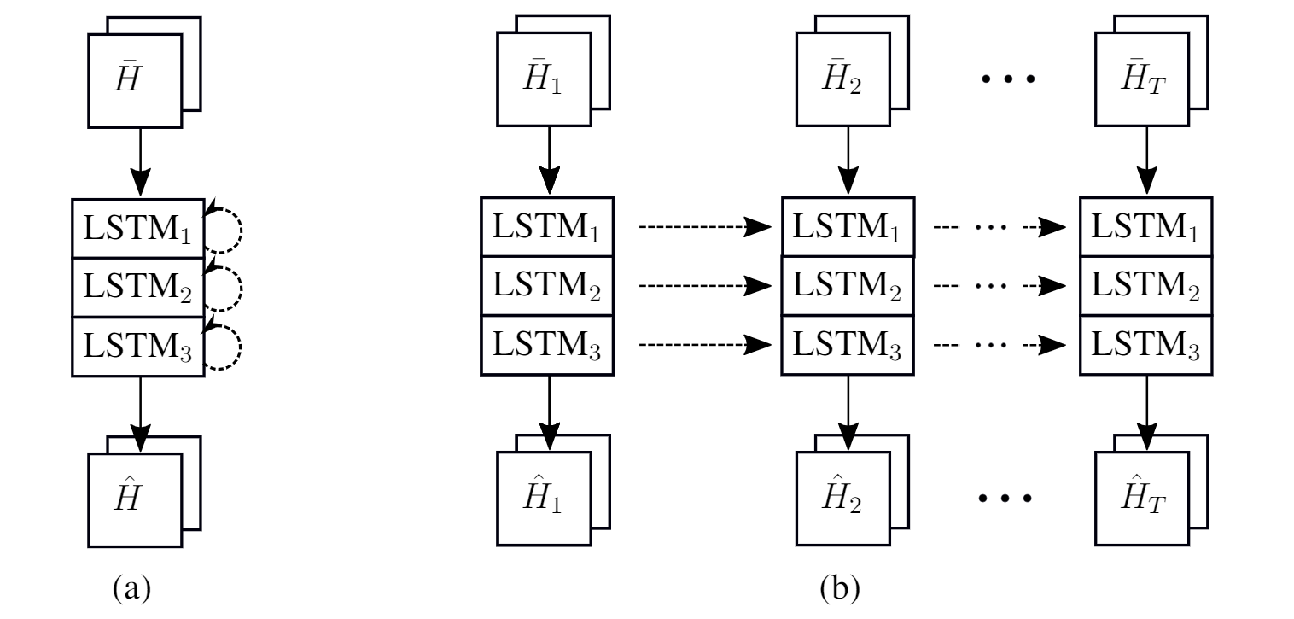
\includegraphics[width=.9\textwidth]{lstm-example-unroll.pdf}
	\medskip
	\caption{An example of LSTMs used for CSI estimation. (a) ``Stacked'' LSTM network of depth 3 shown with recurrent connections. (b) Same LSTM network ``unrolled" into $T$ timeslots }
	\label{fig:lstm_example}
\end{figure}

RNNs have been used extensively in natural language processing (NLP) for machine translation \cite{ref:Sutskever2014seq2seq} and sentiment extraction \cite{ref:Irsoy2014opinion}. For such works in NLP, authors have empirically found ``stacked'' or ``deep'' RNNs to be effective (e.g., Fig.~\ref{fig:lstm_example}), hypothesizing that having multiple recurrent layers allows the network to extract different semantic timescales \cite{ref:Irsoy2014opinion, ref:Bengio2009Learning}. Works in CSI estimation have taken cues from this work in NLP, proposing CSI estimation networks with stacked LSTMs after a sequence of autoencoders \cite{ref:Wang2019CsiNetLSTM}. While such work has demonstrated the utility of RNNs, the computational cost of LSTMs can be prohibitively high. For example, the RNN portion of the network proposed in \cite{ref:Wang2019CsiNetLSTM} accounts for $10^8$ additional parameters (see Figure~\ref{fig:csinet_lstm_arch} for the network architecture used in \cite{ref:Wang2019CsiNetLSTM}). Since channel estimation should not place an undue computational burden on the communications system, LSTMs can be problematic.

\begin{figure}[htb]
	\centering
	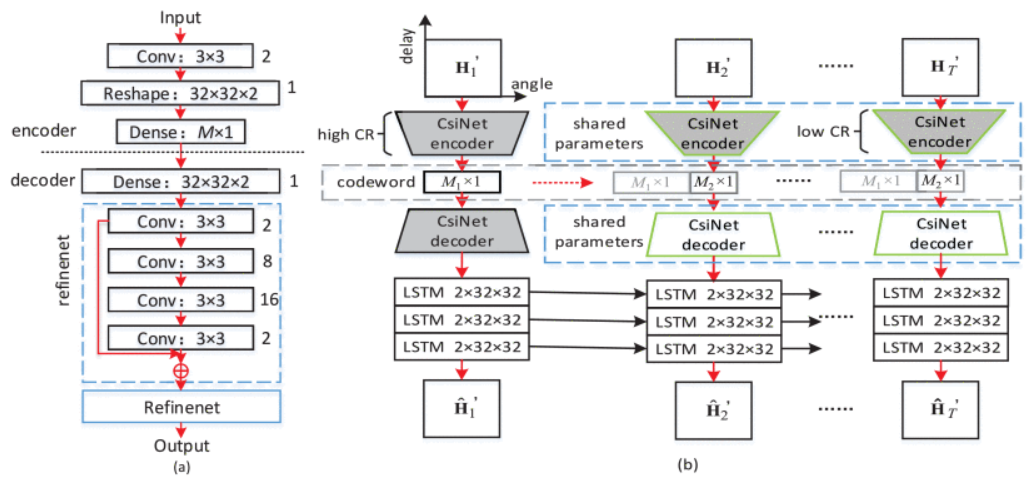
\includegraphics[width=.9\textwidth]{csinet-lstm-arch.png}
	\caption{CsiNet-LSTM architecture from \cite{ref:Wang2019CsiNetLSTM}. (a) CsiNet architecture used in each timeslot. (b) Full CsiNet-LSTM architecture using shared codewords and stacked LSTM cells after CsiNets to extract temporal correlation between timeslots.}
	\label{fig:csinet_lstm_arch}
\end{figure}

\section{Differential Encoding} \label{sect:diff-enc}

Rather than use RNNs to extract temporal dependencies in CSI data, we proposed a lightweight network based on the principle of differential encoding. We trained a network to estimate the error (\ref{eq:diff_err}) under a linear estimator, 
\begin{align*}
	\grave{\mathbf H}_i &=  \hat{\mathbf H}_{i-1} \mathbf W
\end{align*}
where $\mathbf W \in \mathbb C^{R_b \times R_b}$ is the minimum mean squared error (MMSE) estimator,
\begin{align*}
	\mathbf H_i &= \mathbf H_{i-1}\mathbf W + \mathbf E_i \\
	\mathbf H_{i-1}^H\mathbf H_i &= \mathbf H_{i-1}^H\mathbf H_{i-1} \mathbf W + \cancelto{\mathbf 0}{\mathbf H_{i-1}^H\mathbf E_i},
\end{align*}
where the cancellation of the product $\mathbf H_{i-1}^H\mathbf E_i$ is due to the principle of orthogonality (i.e., the error terms are orthogonal to the observed data). Denoting the cross correlation matrix as $\mathbf R_{i} = \mathbb{E}\left[\mathbf H_{t-i}^H\mathbf H_{t}\right]$, we solve for the MMSE estimator,
\begin{align*}
	\mathbf W &= \mathbf R_0^{-1} \mathbf R_1.
\end{align*}
In practice, the population correlation matrices are estimated
via finite samples of size $N$,
\begin{align*}
	\mathbf{\hat R}_k &= \frac {1}{N_{\text{train}}} \sum_{j}^{N_\text{train}} \mathbf H_{i-k}^H(j)\mathbf H_{i}(j),
\end{align*}
where $\mathbf H_i(j)$ is the $j$-th sample in the training set.
The MMSE estimator based on the sample correlation matrices is written as
\begin{align*}
	\hat{\mathbf W} &= \hat{\mathbf R}_0^{-1} \hat{\mathbf R}_1.
\end{align*}
In Appendix~\ref{appdx:autoregressive}, we describe the general multivariate autoregressive model which depends on $\hat{\mathbf{W}}$\footnote{Furthermore, Appendix~\ref{appdx:autoregressive} discusses this multivariate model for the $p$-step case, i.e. using $p$ previous timeslots rather than a single timeslot as described in this section. However, based on experimental results, models with more than one previous timeslot provided only marginal improvements over the one-step model.}. However, we can simplify this model to use a scalar coefficient, $\gamma \in \mathbb R$, as
% \begin{align*}
%   \hat \gamma &= \frac{\sum_{i=1}^N\text{Trace}(\left[\mathbf H_{t-1}^H(i)\mathbf H_{t}(i)\right])}{\sum_{i=1}^N\Arrowvert\mathbf H_t^H(i) \mathbf H_t(i)\Arrowvert^2},
% \end{align*}
\begin{align}
	\hat \gamma &= \frac{\text{Trace}(\hat{\mathbf R}_1}{\sum_k^{R_d}\sum_l^{N_b}\hat{\mathbf R}_0(k,l)}, \label{eq:gamma-hat}
\end{align}
where $k$ ($l$) are the row (column) indices of the correlation matrices. The estimator in this case is 
\begin{align}
	\grave{\mathbf H}_i &= \hat\gamma \hat{\mathbf H}_{i-1} \label{eq:gamma-estim}.
\end{align}
Under the estimator $\gamma$, we proposed to encode the error, $\mathbf E_t$, using a convolutional autoencoder, $f(\mathbf E_t)$,
\begin{align*}
	\hat{\mathbf E}_i &= g(f(\mathbf E_i, \vec\theta_e), \vec\theta_d),
\end{align*}
where $\mathbf E_i = \mathbf H_i - \gamma\hat{\mathbf H}_{i-1}$. The base station has access to the estimators $\gamma$ and $\hat{\mathbf H}_{i-1}$, and the resulting CSI estimate at $t_i$ is
\begin{align}
	\hat{\mathbf H}_i &= \hat\gamma \hat{\mathbf H}_{i-1} + \hat{\mathbf{E}}_i \label{eq:diff-estim}
\end{align}

\subsection{MarkovNet}

In \cite{ref:Liu2020MarkovNet}, we proposed MarkovNet, a deep differential autoencoder. Each timeslot of MarkovNet uses an instance of CsiNet-Pro with unique parameters. The network at the first timeslot ($t_1$) is trained directly on the CSI (i.e., $\mathbf H_1$). For all subsequent timeslots, $t_i$ for $i \geq 2$, we use the MMSE estimator (\ref{eq:gamma-estim}) to produce an error term $\mathbf E_t$, and the autoencoder in each timeslot is trained to produce an error estimate, $\hat{\mathbf E}_t$. The estimated error is added back per (\ref{eq:diff-estim}) to produce a refined estimate.

\begin{figure}[!hbtp]
    \centering
    {
      \fontsize{6pt}{8pt}
      \def\svgwidth{1.0\columnwidth}
      \input{images/markovnet_schematic.pdf_tex}
    }
    \caption{Abstract architecture for MarkovNet. Networks at $t_i$ for $i \geq 2$ are trained to predict the estimation error, $\mathbf E_i$.}
    \label{fig:markovnet_schema}
\end{figure}

\section{Results} \label{sec:markov-results}

We compare MarkovNet with CsiNet-LSTM \cite{ref:Wang2019CsiNetLSTM} on the indoor and outdoor COST2100 datasets (for details, see Section~\ref{sect:channel_model}). For MarkovNet, we train the network at the first timeslot for 1000 epochs. In each subsequent timeslot, we initialize the network using the weights from the previous timeslot and train for 200 epochs. We use a batch size of 200. We perform a training/testing split of 75k/25k samples, and we estimate $\hat\gamma$ using the training set. To compare the estimation accuracy of each network, we report the NMSE.
%estimate of the previous timeslot with the scalar MMSE estimator, $\gamma$, to produce the error term $\mathbf E_t = \mathbf H_t - \gamma\hat{\mathbf H}_{t-1}$.

\subsection{Network Comparison}

Figure~\ref{fig:diffnet_result} shows the NMSE of MarkovNet and CsiNet-LSTM for four different compression ratios. For the indoor network, all instances of MarkovNet achieve lower NMSE than all instances of CsiNet-LSTM. In the outdoor scenario, each CR for MarkovNet demonstrates lower NMSE than the corresponding CR for CsiNet-LSTM. Between both channel scenarios, MarkovNet shows gradual improvement for subsequent timeslots if the CR is high enough while CsiNet-LSTM only improves gradually in the outdoor environment for CR$=\frac 14$.
\begin{figure}[!hbtp] \centering 
	\begin{subfigure}[t]{.45\textwidth}
		\centering
		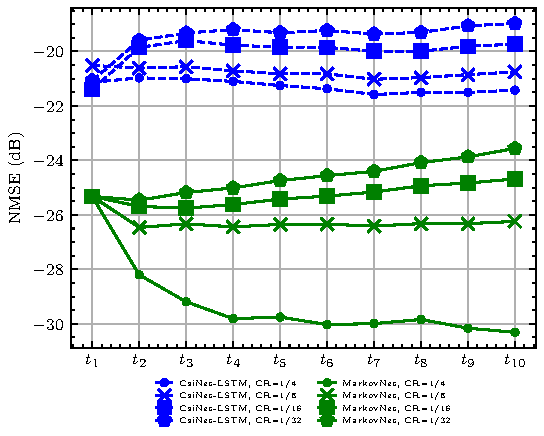
\includegraphics[width=\linewidth]{MarkovNet_truncated_Indoor_10slots.pdf}
		\caption{Indoor}
		\label{fig:diffnet_indoor} 
	\end{subfigure}
	\begin{subfigure}[t]{.45\textwidth}
		\centering
		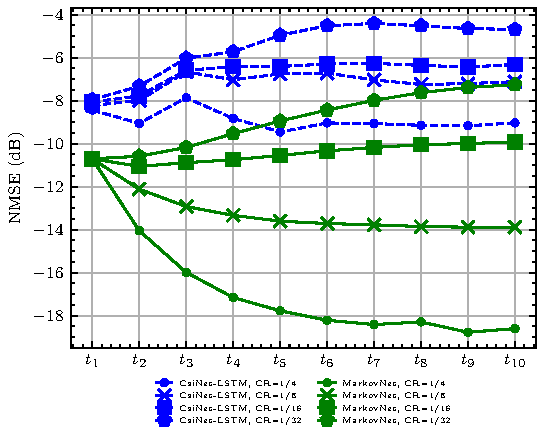
\includegraphics[width=\linewidth]{MarkovNet_truncated_Outdoor_10slots.pdf}
		\caption{Outdoor}
		\label{fig:diffnet_outdoor} 
	\end{subfigure}
	\caption{$\text{NMSE}$ comparison of MarkovNet and CsiNet-LSTM 
	at various compression ratios (CR).} 
	\label{fig:diffnet_result} \vspace*{-2mm}
\end{figure}  
Figure~\ref{fig:csi_image} shows a random sample from the test set, $\mathbf H$, and the estimates produced by CsiNet-LSTM and MarkovNet for a CR of $\frac 14$. This sample contains three ``peak'' magnitude regions. While both networks manage to capture the two larger samples, MarkovNet is able to recover the small peak magnitude region ({\color{darkgreen}green arrow}) which CsiNet-LSTM fails to produce ({\color{red}red arrow}).

\begin{figure}[htb] \centering 
	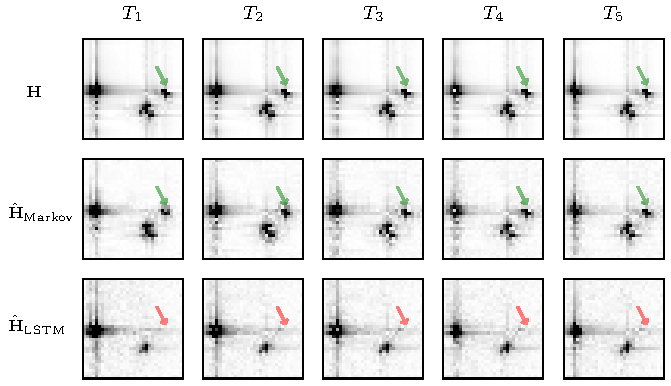
\includegraphics[width=0.9\linewidth]{batch0_csi_compare_cr512_annot.pdf}
	\caption{CSI ($\mathbf H$), MarkovNet estimates ($\hat{\mathbf H}_{\text{Markov}}$), and CsiNet-LSTM estimates ($\hat{\mathbf H}_{\text{LSTM}}$) across five timeslots ($T_1$ through $T_5$) on one outdoor channel sample from the test set,
using $\text{CR}=\frac 14$.} 
	\label{fig:csi_image} 
\end{figure}

\subsection{Performance under Quantization}

To understand the effect of quantization on the network performance, we choose to use $\mu$-law companding and uniform quantization on the latent feedback elements. We begin by performing a logarithmic scaling on the feedback elements, $x$,
\begin{align}
	f(x) = \frac{\text{sign}(x)\ln\left(1 + \mu|x|\right)}{\ln\left(1 + \mu\right)} , \; 0 \leq |x| \leq 1. \label{eq:mu-forward}
\end{align}
After applying (\ref{eq:mu-forward}) to the signal, uniform quantization is applied to yield
\begin{align}
	\hat x = \Delta\left\lfloor\frac{f(x)}{\Delta}\right\rceil \label{eq:unif-quant}
\end{align}
where $\Delta = 2^{-(b-1)}$ for $b$-bit quantization. Finally, an inverse logarithmic scaling is applied to quantized signal,
\begin{align}
	F(\hat x) = \frac{\text{sign}(\hat x)\left(1 + \mu\right)^{|\hat x|} - 1}{\mu} , \; -1 \leq \hat x \leq 1. \label{eq:mu-backward}
\end{align}
In short, the described $\mu$-law quantization scheme involves applying (\ref{eq:mu-forward}), then (\ref{eq:unif-quant}), then (\ref{eq:mu-backward}) to each feedback element. Figures~\ref{fig:feedback_quant_indoor} and~\ref{fig:feedback_quant_outdoor} show the performance of MarkovNet and CsiNet-LSTM under $\mu$-law quantization where $\mu=255$.

In the Outdoor scenario, the performance of each network at each compression ratio does not change substantially for different numbers of quantization bits. In contrast, the performance for each network/compression ratio in the Indoor scenario drops appreciably for smaller quantization bits. We note that the performance of either network could potentially benefit from quantization during training, as all the results in Figures~\ref{fig:diffnet_indoor} and~\ref{fig:diffnet_outdoor} are trained with continuous feedback.

\begin{figure}[!hbtp] \centering 
	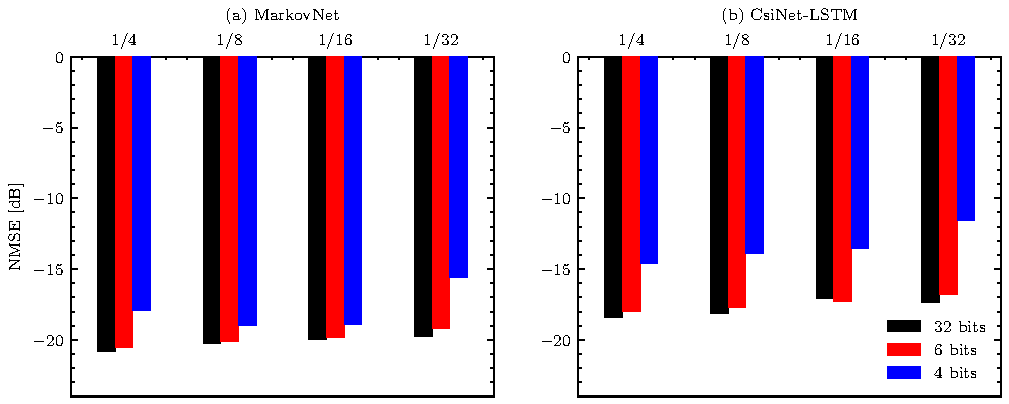
\includegraphics[width=\textwidth]{Indoor_feedback_quant.pdf}
    \caption{NMSE comparison of MarkovNet and CsiNet-LSTM for the Indoor scenario with feedback subject to $\mu$-law quantization using fixed step size, $\Delta=2^{-(b-1)}$, for $b$ bits.}
	\label{fig:feedback_quant_indoor} \vspace*{-2mm}
\end{figure}

\begin{figure}[!hbtp] \centering 
	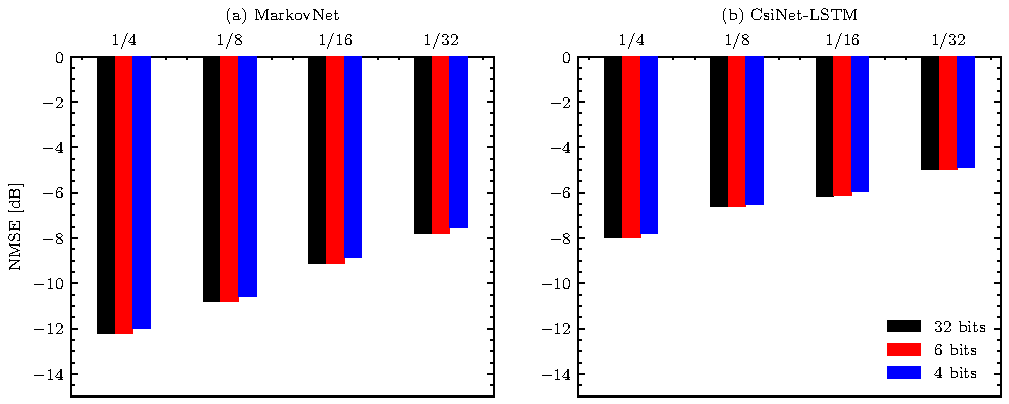
\includegraphics[width=\textwidth]{Outdoor_feedback_quant.pdf}
    \caption{NMSE comparison of MarkovNet and CsiNet-LSTM for the Outdoor scenario with feedback subject to $\mu$-law quantization using fixed step size, $\Delta=2^{-(b-1)}$, for $b$ bits.}
	\label{fig:feedback_quant_outdoor} \vspace*{-6mm}
\end{figure}

\subsection{Computational Complexity}

The resulting network requires no recurrent layers, resulting in a substantial reduction in computational complexity. Table~\ref{tab:comp-complex} shows the number of parameters and FLOPs per timeslot for CsiNet-LSTM, MarkovNet, and CsiNet. The parameter count of MarkovNet is on par with CsiNet, and CsiNet-LSTM requires orders of magnitude more parameters. While the number of FLOPs for MarkovNet is nearly 10 times smaller than CsiNet-LSTM, MarkovNet requires 5 to 10 times more FLOPs than CsiNet due to the increased kernel size of CsiNet-Pro.

\begin{table}[htb]
  \renewcommand{\arraystretch}{1}
  \begin{center}
  % \caption{Table II: Model size \& computational complexity comparison. M: million, K: thousand.}
  \caption{Model size/computational complexity of tested temporal networks (CsiNet-LSTM, MarkovNet) and comparable non-temporal network (CsiNet). M: million.}
  \label{tab:comp-complex} 
  % \resizebox{\linewidth}{15mm}
  \footnotesize{
	  \begin{tabular}{|l|c|c|c|c|c|c|}
	  \hline
	                              & \multicolumn{3}{c|}{\textbf{Parameters}} & \multicolumn{3}{c|}{\textbf{FLOPs}} \\ \hline
	                              & \textbf{CsiNet-LSTM} & \textbf{MarkovNet} & \textbf{CsiNet} & \textbf{CsiNet-LSTM} & \textbf{MarkovNet} & \textbf{CsiNet} \\ \hline
	  \textbf{CR=$1/4$}  		  & 132.7 M              & 2.1 M              & 2.1 M  			& 412.9 M              & 44.5 M             & 7.8 M           \\ \hline
	  \textbf{CR=$1/8$}  		  & 123.2 M              & 1.1 M              & 1.1 M  			& 410.8 M              & 42.	4 M             & 5.7 M           \\ \hline
	  \textbf{CR=$1/16$} 		  & 118.5 M              & 0.5 M              & 0.5 M 			& 409.8 M              & 41.3 M             & 4.7 M           \\ \hline
	  \textbf{CR=$1/32$} 		  & 116.1 M              & 0.3 M              & 0.3 M           & 409.2 M              & 40.8 M             & 4.1 M           \\ \hline
	  \textbf{CR=$1/64$} 		  & 115.0 M              & 0.1 M              & 0.1 M 			& 409.0 M              & 40.5 M             & 3.9 M           \\ \hline
	  \end{tabular}
  }
  \end{center}
\end{table} 
\chapter{Spectrum-efficient Pilot-based CSI Feedback}
\label{chap:p2d}

This chapter details an estimator for the UE-side angular-delay domain CSI based on a limited number of spatial-frequency domain pilots. This scheme adheres to the 3GPP standards for pilot allocation across time-frequency resources as described in Section~\ref{sect:pilots}.

Section~\ref{sect:p2de} details our proposed pilots-to-delay estimator (P2DE), and Figure~\ref{fig:p2d} demonstrates the operating principle behind P2DE. Appendix~\ref{appdx:odir} describes off-diagonal regularization as a countermeasure for ill-conditioned CSI matrices. Section~\ref{sect:diag} explicitly links the proposed P2DE to the 3GPP placement of CSI-RS/DMRS resource elements and describes our proposed diagonal pilot pattern which adheres to LTE/NR specifications. Section~\ref{sect:hetero-markov} describes an extension of our previously proposed differential encoding network which uses heterogeneous CNNs for different timeslots. Finally, Section~\ref{sect:p2de-results} presents results for the P2DE and our propose heterogeneous differential encoding networks.

\begin{figure}[!hbtp]
    \centering
    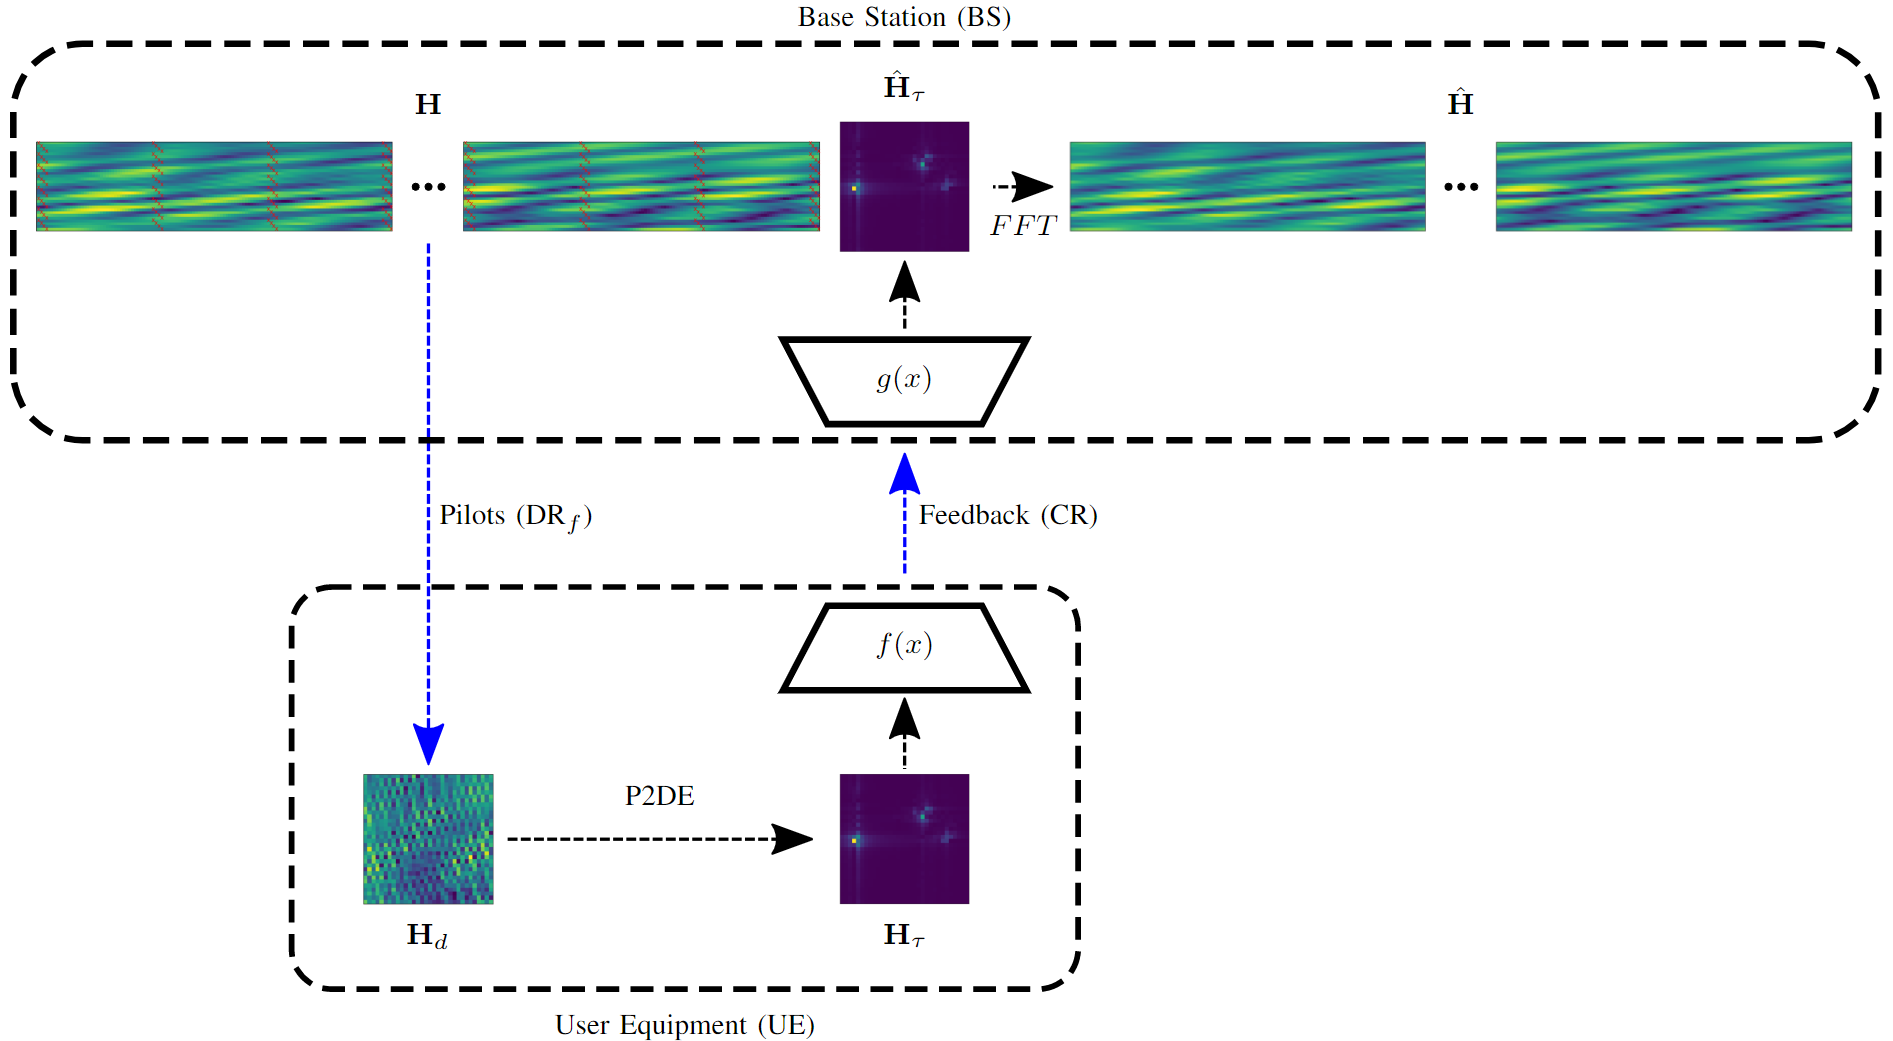
\includegraphics[width=\linewidth]{./images/00_downlink_p2d_feedback_horiz_diag.png}
    \caption{Compressive CSI estimation based on linear P2D estimator. First,
    we use downlink pilots to 
    generate a sparse, frequency domain CSI
    estimate 
    of size $M_f << N_f$. We then apply
    the P2D estimator, $\mathbf{Q}^\dag_{N_t}$ of (\ref{eq:p2d_short}), to establish 
    the truncated
    delay domain CSI estimate.
    We train a
    learnable encoder, 
    $f(x)$,
    and decoder, $g(x)$, to compress and decode the feedback, respectively. The 
    gNB recovers
    the frequency domain
    CSI from 
    the decoded 
    delay domain CSI estimate.}
    \label{fig:p2d}
\end{figure}

\section{Pilots-to-delay Estimator (P2DE)}
\label{sect:p2de}

Denote $\boldeta_i \in \mathbb{C}^{N_f}$ as the $i$-th row of the spatial-frequency matrix $\mathbf{H}$, and denote the downsampled version of $\boldeta_i$ as $\boldeta_{d,i} \in \mathbb{C}^{M_f}$ where $M_f << N_f$. Thus, the spatial-frequency CSI, $\mathbf{H}$, and its downsampled counterpart, $\mathbf{H}_d$, can be written as,
\begin{equation}
	\mathbf{H} = \begin{bmatrix} \boldeta_1 \\ \boldeta_2 \\ \vdots \\ \boldeta_{N_b} \\\end{bmatrix}\in\mathbb{C}^{N_b \times N_f}, \; \mathbf{H}_d = \begin{bmatrix} \boldeta_{d,1} \\ \boldeta_{d,2} \\ \vdots \\ \boldeta_{d,N_b} \\\end{bmatrix}\in\mathbb{C}^{N_b \times M_f}.
\end{equation}
$\boldeta_{d,i}$ is related to $\boldeta_i$ by the downsampling matrix for the $i$-th antenna port, $\mathbf{P}_i$, as
\begin{equation}
	\boldeta_{d,i} = \boldeta_i \mathbf{P}_i \; \forall \; i \in [1, \dots, N_b].
\end{equation}
Denote the delay-domain CSI vector, $\tilde{\boldeta}_i$, which is defined as
\begin{equation}
	\tilde{\boldeta}_{i}\mathbf{F} = \boldeta_i, \label{eq:dft}
\end{equation}
where $\mathbf{F}$ is the $\mathbf{C}^{N_f \times N_f}$ discrete Fourier transform (DFT) matrix. To relate the frequency domain pilots to the delay domain, we apply the pilot downsampling matrix $\mathbf{P}_i$ to both sides of (\ref{eq:dft}),
\begin{align}
	\tilde{\boldeta}_{i}\mathbf{F}\mathbf{P}_i = \boldeta_i\mathbf{P}_i \nonumber \\
	\tilde{\boldeta}_{i}\mathbf{Q}_i = \boldeta_{d,i} \label{eq:qmat}
\end{align}
where $\mathbf{Q}_i=\mathbf{F}\mathbf{P}_i\in\mathbb{C}^{N_f\times M_f}$ is the downsampled DFT matrix.
Leveraging the sparsity of CSI data in the delay domain (see Section~\ref{sect:sparse-csi}, Figure~\ref{fig:freq-vs-delay}), many works choose to feedback and compress the truncated delay domain vectors, $\tilde{\boldeta}_{c,i}\in\mathbb{C}^{N_t}$. The zero-padded vector $\tilde{\boldeta}_{i}$ defined as
\begin{align} 
	\tilde{\boldeta}_{i} = \left[\tilde{\boldeta}_{c,i}, \mathbf{0}_{N_f - N_t}\right]. \label{eq:p2d_short}
\end{align}

Based on \ref{eq:qmat}, the delay domain can be related directly to the pilots by taking the pseudoinverse,
\begin{align}
	\tilde{\boldeta}_{i}\mathbf{Q}_i\mathbf{Q}_i^T &= \boldeta_{d,i}\mathbf{Q}_i^T \nonumber \\
	\tilde{\boldeta}_{i} &= \boldeta_{d,i}\mathbf{Q}_i^T\left(\mathbf{Q}_i\mathbf{Q}_i^T\right)^{-1} \nonumber \\
	&= \boldeta_{d,i}\mathbf{Q}_i^{\#} \label{eq:p2d}
\end{align}

% \subsection{Regularization of P2DE} \label{sect:odir}

When the pilot patterns $\mathbf{P}_i$ are equidistant and regularly spaced, the P2DE matrices $\mathbf{Q}_i\mathbf{Q}_i^T$ are typically well-conditioned. However, more irregular patterns can result in ill-conditioned matrices $\mathbf{Q}_i\mathbf{Q}_i^T$, making these matrix inversions unstable. To compensate for this ill-conditioning, we propose to use off-diagonal regularization (ODIR) to condition the P2DE matrices. This form of regularization is described in more detail in Appendix~\ref{appdx:odir}. 

\begin{figure}[!hbtp]
    \centering
    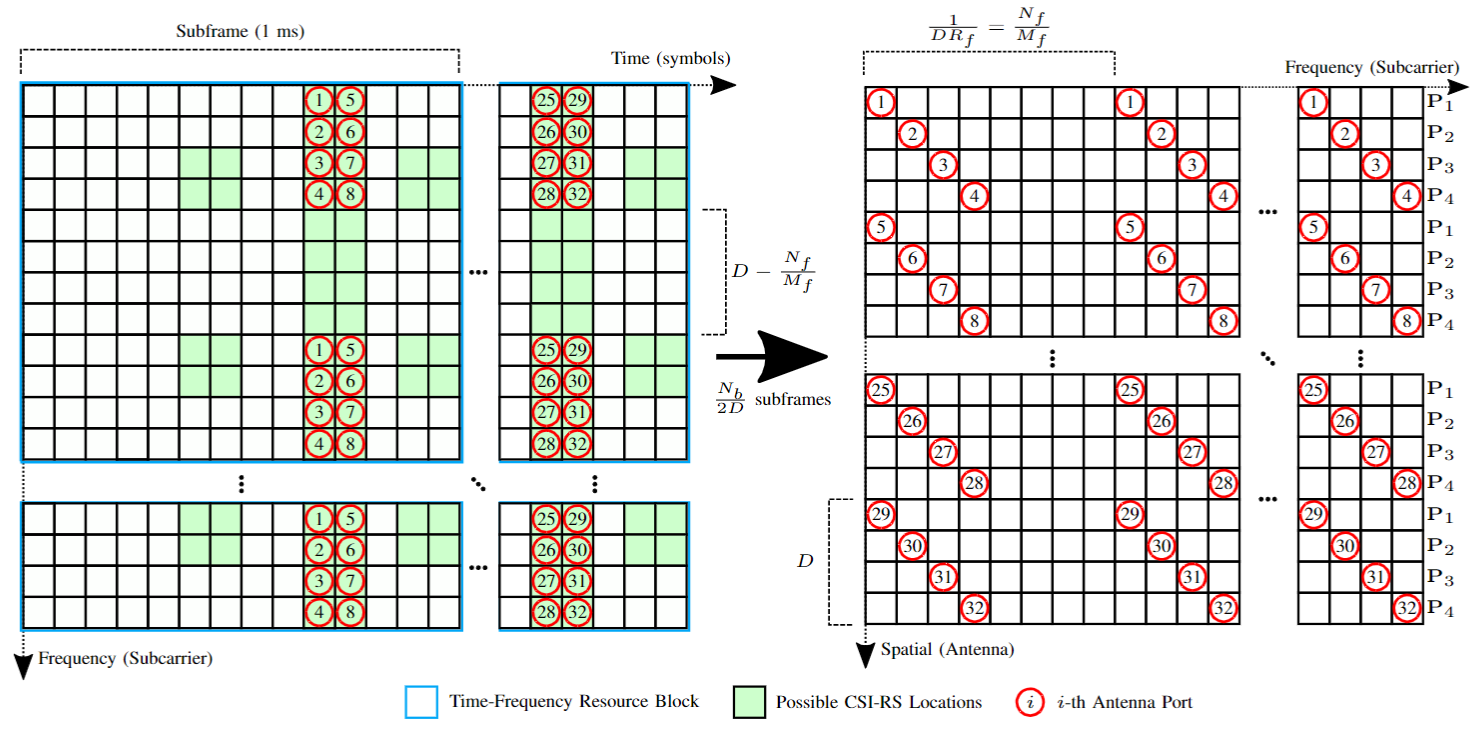
\includegraphics[width=\linewidth]{images/01_p2d_pilots_diag_with_resource_grid.png}
    \caption{(a) LTE Resource Blocks and CSI-RS locations where antenna port pilots are allocated. (b) Schematic for diagonal pilots with relevant parameters, size of diagonal $D$ and frequency downsampling ratio $\text{DR}_f$. In this diagram, $N_b=32, D=4, \text{DR}_f=\frac 18$. The pilot matrix $\mathbf{P}_j$ indicates the downsampling pattern for the $j$-th element of the diagonal pattern. The number of subframes necessary to populate (b) is inversely proportional to $D$.}
    \label{fig:p2d_diag}
\end{figure}

\subsection{Diagonal Pilot Allocations for 3GPP Standards} \label{sect:diag}

As discussed in Section~\ref{sect:pilots}, 3GPP specifications describe the allocation of pilots to time-frequency resources in 4G/LTE \cite{ref:3gpp.36.211, ref:Asplund2020} and 5G/NR \cite{ref:3GPPTS38.211V15.8.0} radio networks, where the reserved resource elements are called CSI reference signals (CSI-RS) for the former and demodulation reference signals (DMRS) for the latter.

In order to connect the P2DE as described in Section~\ref{sect:p2de} to the 3GPP specifications, we must specify the corresponding pilot patterns in the time-frequency grid. In Figure~\ref{fig:p2d_diag}, we show an example of our proposed `diagonal' pilot pattern in an LTE network using CSI-RS locations. We refer to this pattern as diagonal since it is diagonal in the spatial-frequency domain. The benefit of the diagonal pattern can be understood by considering the time needed to acquire downsampled CSI matrix, $\mathbf{H}_d$.

\begin{figure}[!hbtp]
    \centering
    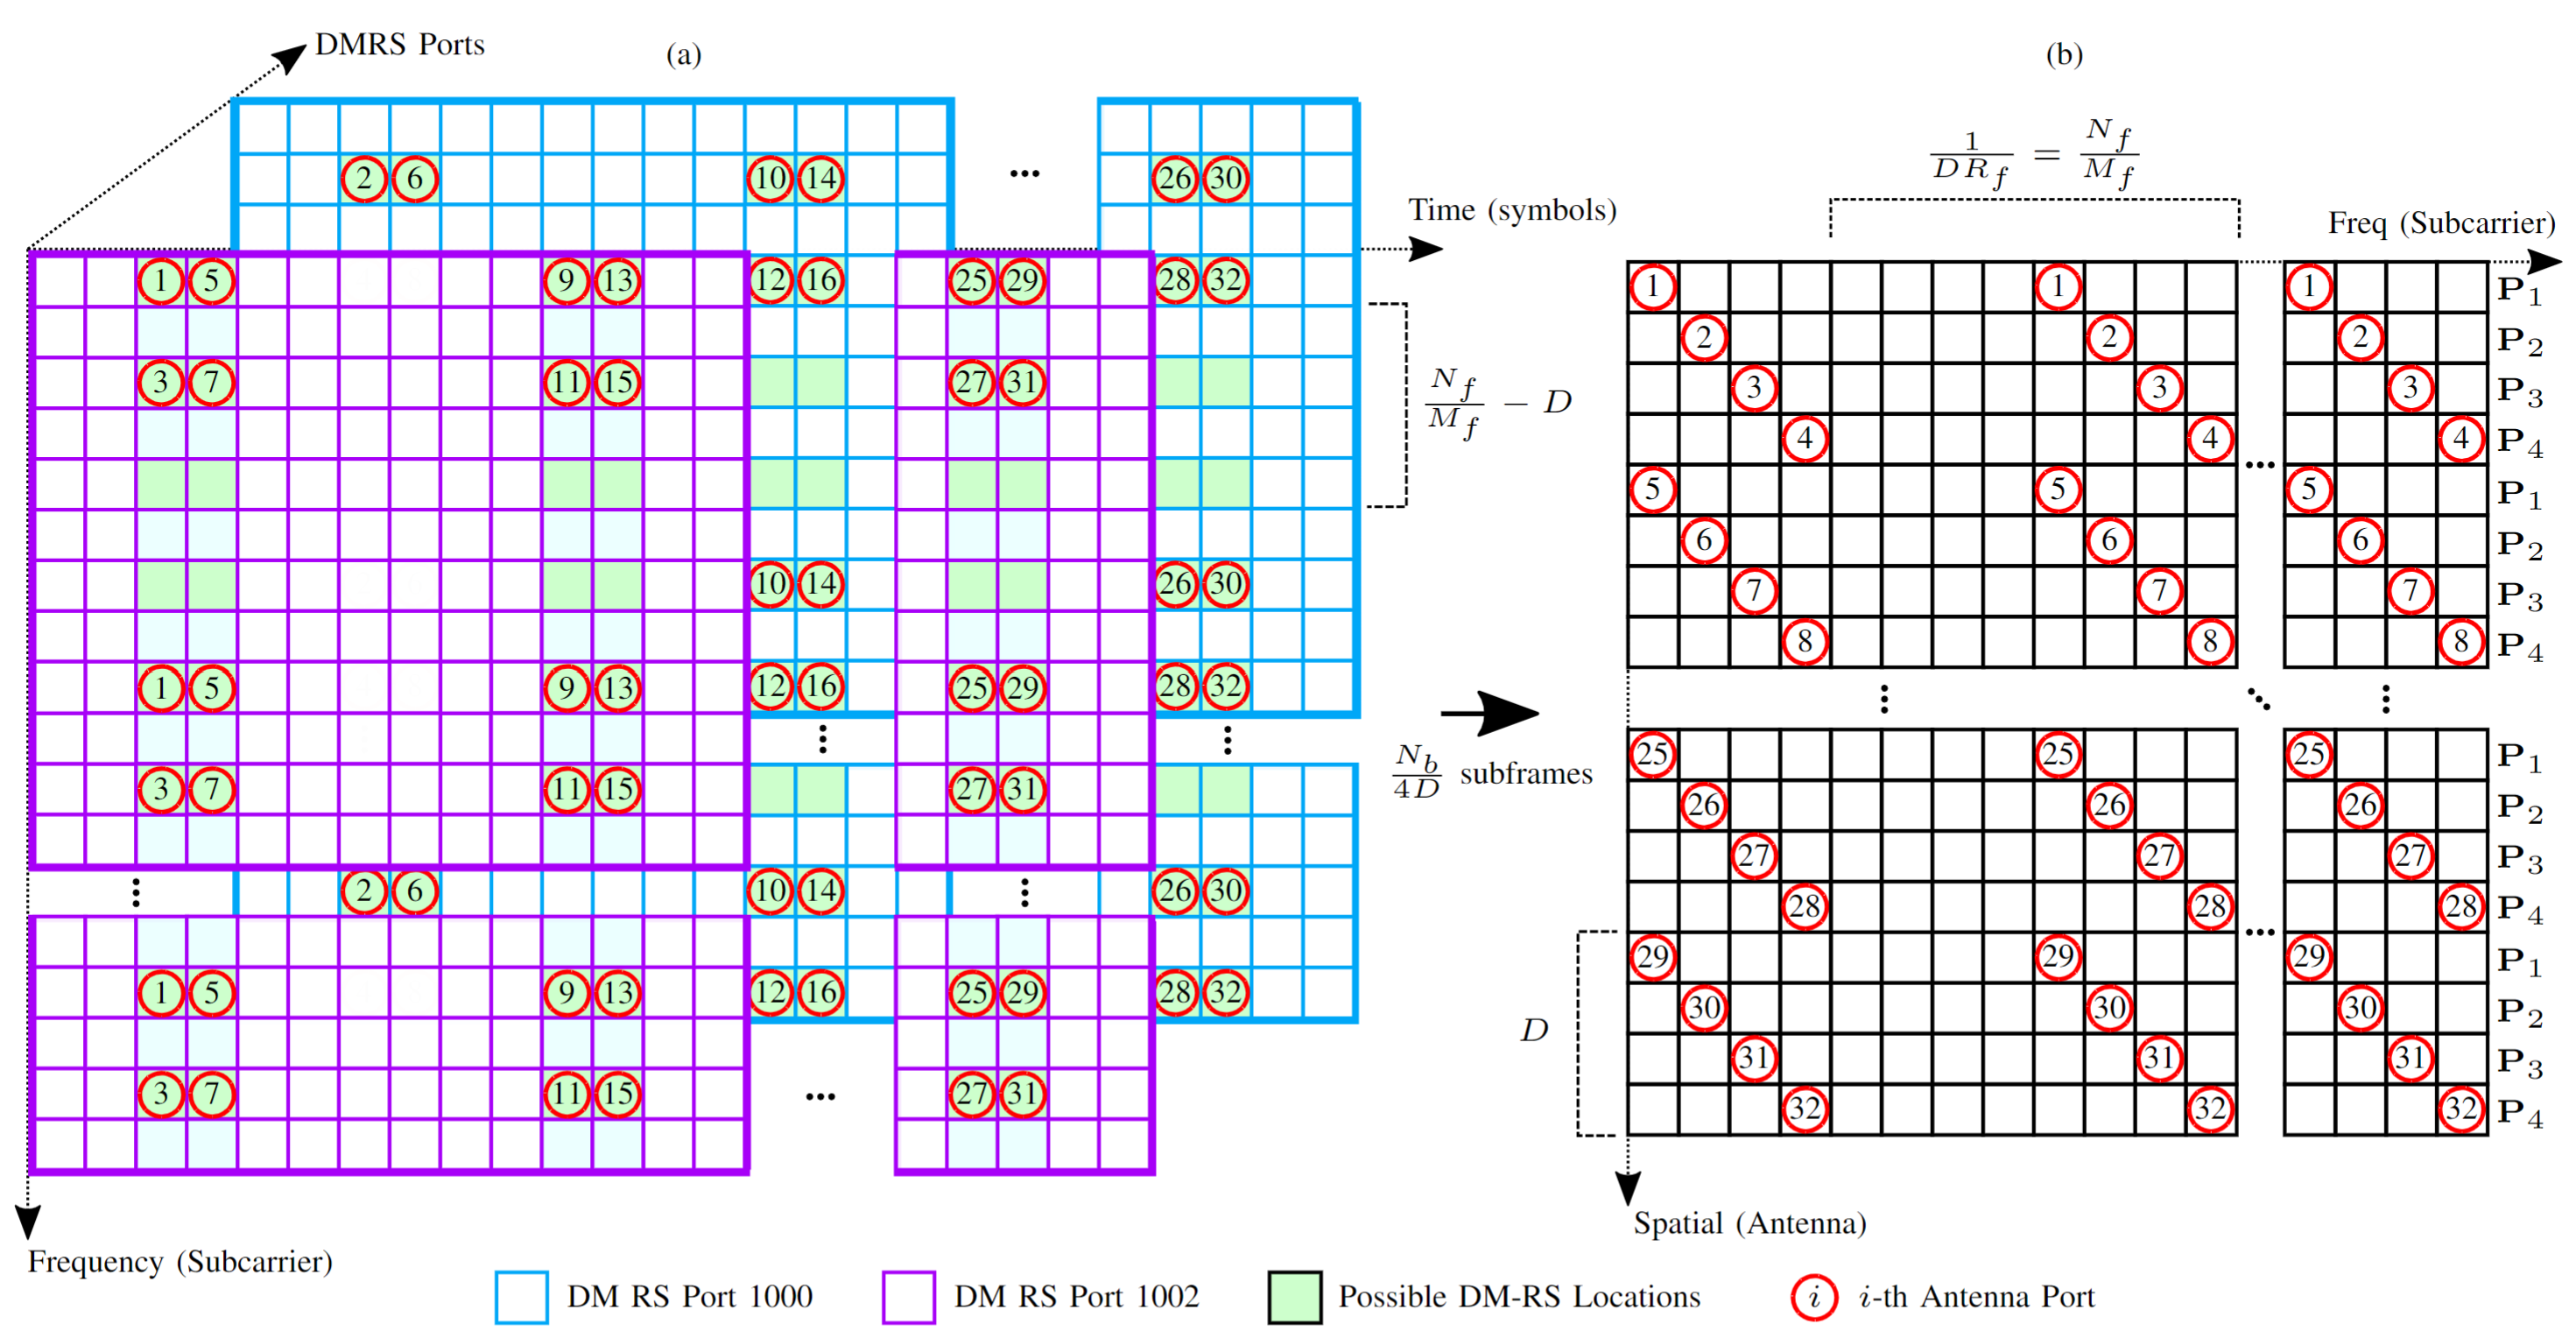
\includegraphics[width=\linewidth]{images/03_p2d_pilots_diag_with_resource_grid_5gnr_ortho.png}
    \caption{(a) 5G NR Resource Blocks and DMRS locations where antenna port pilots are allocated. (b) Schematic for diagonal pilots with relevant parameters, size of diagonal $D$ and frequency downsampling ratio $\text{DR}_f$. In this diagram, $N_b=32, D=4, \text{DR}_f=\frac 18$. The pilot matrix $\mathbf{P}_j$ indicates the downsampling pattern for the $j$-th element of the diagonal pattern. The number of subframes necessary to populate (b) is inversely proportional to $D$.}
    \label{fig:p2d_diag_5gnr}
\end{figure}

Algorithm~\ref{alg:p2d-diag} shows the process for acquiring the delay domain P2DE from sparse frequency domain pilots.

\begin{algorithm}
    \caption{Pilots-to-delay Estimator (P2D) for Diagonal Pilot Pattern} 
    \label{alg:p2d-diag}
    \begin{algorithmic}[1]
    \State \textbf{\emph{Input}}:
        P2DE Matrices, $\mathbf{Q}_{c,j}^\#,\;
        j\in\{1,\dots, D\}$
    \State \textbf{\emph{Input}}: Pilot spatial-frequency CSI, $\mathbf{H}_d\in\mathbb{C}^{N_b\times M_f}$
    \State \textbf{\emph{Initialize}}: Spatial-delay CSI, $\tilde{\mathbf{H}}_\tau\in\mathbb{C}^{N_b\times N_t}$
   \State \textbf{\emph{Initialize}}: Angular-delay CSI estimate, ${\mathbf{H}}_\tau
              \in\mathbb{C}^{N_b\times N_t}$
   \For {$i=1,2,\ldots, N_b$}
        \State \textbf{\# \emph{Index for $j$-th pilot matrix}}
        \State $j = ((i-1) \text{ mod } D) + 1$
        \State \textbf{\# \emph{Apply P2D to $i$-th antenna port}}
        \State ${\boldeta}_{d,i} = \mathbf{H}_d(i,:)$
        \State $\tilde{{\mathbf{H}}}_{\tau}(i,:) = {\boldeta}_{d,i}\mathbf{Q}^{\#}_{c,j}$
        \EndFor
        \State \textbf{\# \emph{Convert from spatial to angular}}
        \State ${{\mathbf{H}}}_{\tau}=\mathbf{F}_{N_b}\tilde{{\mathbf{H}}}_{\tau}$
        \State \textbf{\emph{Return}} ${{\mathbf{H}}}_{\tau}$
    \end{algorithmic} 
\end{algorithm}

\section{Heterogeneous Differential Encoding with P2DE}
\label{sect:hetero-markov}

Chapter~\ref{chap:markovnet} introduced the concept of differential encoding for CSI feedback compression. The delay domain P2DE CSI introduced in this chapter can also be used in the differential encoding framework. Figure~\ref{fig:markov-p2d} showcases the data path when utilizing the P2D estimates with a differential encoding network.

The prior work proposed a differential encoding network that used an identical autoencoder at each timeslot. We refer to such a network as `homogeneous.' In contrast, we can consider a `heterogeneous' network, where we use different network architectures at different timeslots.

In this section, we describe a heterogeneous differential encoder which combines deep compressed sensing with deep autoencoders.

\begin{figure}[!hbtp]
    \centering
    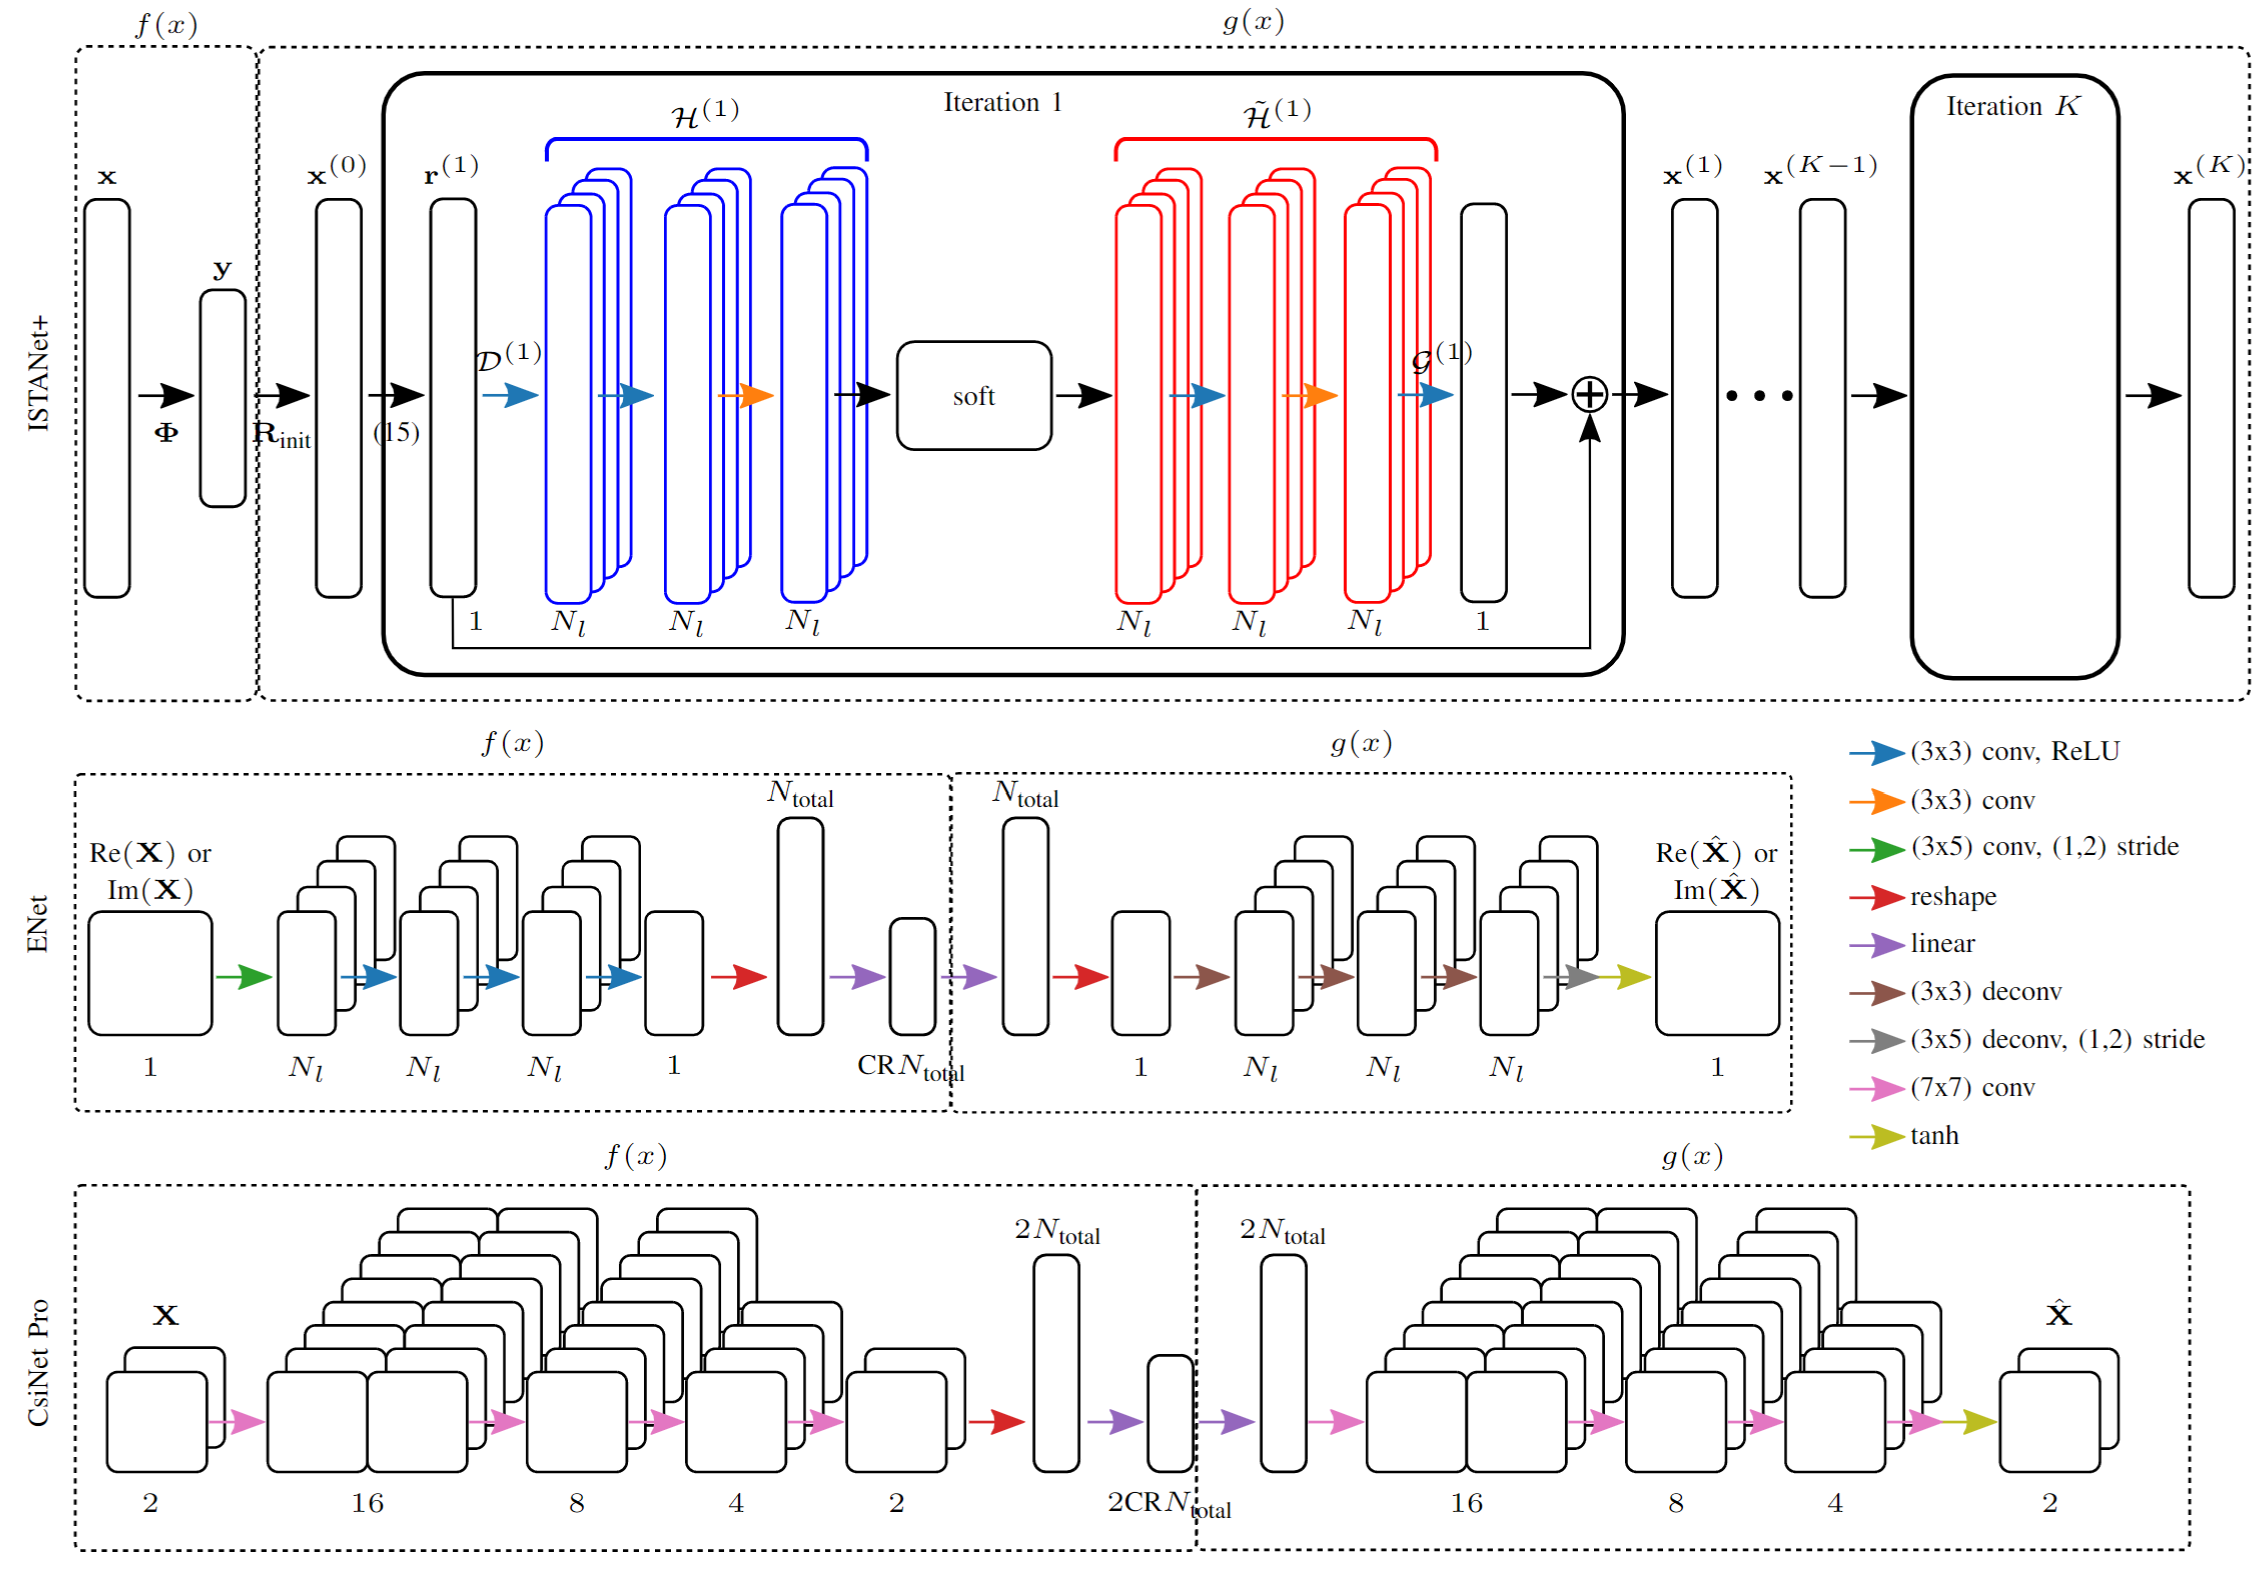
\includegraphics[width=\linewidth]{images/arch-comparison.png}
    % \input{figure/csinet_quant.pdf_tex}
    \caption{Compressive CSI estimation architectures used in this work. $f(x)$ denotes the encoder, and $g(x)$ denotes the decoder. $N_{\text{total}}=N_bN_t$ is the size of the real or imaginary channel. $N_l$ is the number of latent channels in a convolutional layer.}
    \label{fig:arch_compare}
\end{figure}

\subsection{Iterative Optimization Networks for Compressed Sensing-based CSI Feedback} \label{sec:iter-cs}

% In \cite{ref:zhang2018ista}, the authors emulate the iterations of the Iterative Shrinkage-Thresholding Algorithm (ISTA) as lightweight CNNs. They propose a network (ISTANet+) which utilizes skip connections in each iteration to learn the residual of the reconstructed image.
 
While CNN autoencoders have been dominant in CSI estimation, recent work from image processing has shown promise in using trainable CS algorithms based on CNNs\footnote{For an overview of conventional compressed sensing solutions as well as the original ISTA algorithm, see Appendix~\ref{appdx:compressed-sensing}}. These works treat iterative CS algorithms as sequential networks by ``unrolling'' them into discrete blocks \cite{ref:yang2016deep, ref:zhang2018ista}. Investigating unrolled CS algorithms for CSI estimation warrants consideration, as CS algorithms can have guaranteed convergence under mild sparsity conditions (in contrast with CNNs autoencoder approaches, which do not have such guarantees). Since CSI data exhibits sparsity in the delay domain, specifying an appropriate compressed sensing approach could provide appreciable performance gains in our differential CSI encoding architecture. 

To exploit the temporal coherence of the MIMO channel, we propose to construct a differential encoding network using an unrolled optimization network based on a trainable version of the iterative shrinkage-thresholding algorithm (ISTA), called ISTANet+ \cite{ref:zhang2018ista}. See the top of Figure~\ref{fig:arch_compare} for a diagram of ISTANet+. Denote measurement matrix for the ISTANet+ as 
\begin{align}
    \mathbf \Phi \in \mathbf{R}^{N_{\text{total}}\text{CR} \times N_{\text{total}}}.
\end{align}
For compressed sensing approaches, the measurement matrix is analogous to the `encoder' of autoencoder approaches, i.e., $f(x)=\mathbf\Phi x$. The `decoder' consists of $K$ iterations of the following update steps,
\begin{align}
    \mathbf{r}^{(k)} &= \mathbf{x}^{(k-1)}-\rho^{(k)}\mathbf{\Phi}^\top(\mathbf{\Phi}\mathbf x^{(k-1)}-\mathbf y) \label{eq:istanet-grad} \\
    % \mathbf x^{(k)} &= \tilde{\mathcal{F}}^{(k)}\left(\text{soft}\left(\mathcal{F}^{(k)}(\mathbf{r}^{(k)}), \theta^{(k)}\right)\right)
    \mathbf x^{(k)} &= \mathbf{r}^{(k)} + \mathcal{G}^{(k)}\left(\tilde{\mathcal{H}}^{(k)}\left(\text{soft}\left(\mathcal{H}^{(k)}(\mathcal{D}^{(k)}(\mathbf{r}^{(k)}), \theta^{(k)}\right)\right)\right) \label{eq:istanet-prox}
\end{align}
where $\mathbf y=\mathbf{\Phi} \mathbf x$, $\mathbf x^{(0)}=\mathbf{R}_{\text{init}}\mathbf{y}$, and $\mathbf R_{\text{init}}=\mathbf {XY}(\mathbf{YY}^\top)^{-1}$ is the initialization matrix for the training data matrix $\mathbf X = \left[\mathbf{x}_1, \mathbf{x}_2,\dots, \mathbf{x}_{N_{\text{train}}}\right]$ and the training measurement matrix $\mathbf Y = \left[\mathbf{y}_1, \mathbf{y}_2,\dots, \mathbf{y}_{N_{\text{train}}}\right]$. `soft($\cdot$)' denotes the soft threshold function,
\begin{align}
    \text{soft}(x, \theta) &= \text{sign}(x)\text{ReLU}(|x|-\theta). \label{eq:soft}
\end{align}
$\mathcal G^{(k)}, \mathcal D^{(k)},  \mathcal H^{(k)}, \tilde{\mathcal H}^{(k)}$ indicate trainable nonlinear mappings (in this case, CNNs), and $\mathcal H^{(k)}, \tilde{\mathcal H}^{(k)}$ are subject to the symmetry constraint $\mathcal H^{(k)}\circ \tilde{\mathcal H}^{(k)}=\mathbf I$. The rectified linear unit (ReLU) is given as
\begin{align*}
    \text{ReLU}(x) &= 
        \begin{cases}
            x & x \geq 0 \\
            0 & x < 0
        \end{cases}
\end{align*}
In the proposed differential encoding scheme, we use an instance of ISTANet+ in the first timeslot, $t_1$, with a large compression ratio such that $\text{CR}_{t_1} \geq \text{CR}_{t_i}$ for all $i > 1$. This choice in compression ratio allows us to initialize the network with a high-quality estimate at the first timeslot. Notably, the training data matrix, $\mathbf X$, differs between timeslots. For the first timeslot, the data vectors $\mathbf{x}_i$ are vectorized versions of the CSI matrices,
\begin{align}
    \mathbf{x}_j &= \text{vec}\left(\mathbf{H}^{(j)}_{\tau,1}\right) \text{ for } j\in[N_{\text{train}}]. 
    \label{eq:t1_vec}
\end{align}
However, the data vectors for all other timeslots are vectorized versions of the error matrices,
\begin{align}
    \mathbf{x}_j &= \text{vec}\left(\bar{\mathbf{E}}^{(j)}_{i}\right) \text{ for } j\in[N_{\text{train}}]. 
    \label{eq:ti_vec}
\end{align}
Denote the parameters for ISTANet+ in the $t_i$-th timeslot as $\mathbf{\Theta}_{t_i}=\{\mathcal G^{(k)}, \mathcal D^{(k)},  \mathcal H^{(k)}, \tilde{\mathcal H}^{(k)}, \theta^{(k)}, \rho^{(k)}\}_{k=1}^{K}$. The loss function is a weighted sum of the MSE and the symmetry constraint, i.e.,
\begin{align}
    L(\mathbf{\Theta}_{t_i}) &= L_{\text{MSE}} + \alpha L_{\text{sym}} \\
    L_{\text{MSE}} &= \frac{1}{N_{\text{batch}}N_{\text{total}}}\sum_{i=1}^{N_{\text{batch}}}\|\mathbf{x}_i^{(K)}-\mathbf{x}_i\|_2^2 \\
    L_{\text{sym}} &= \frac{1}{N_{\text{batch}}N_{\text{total}}}\sum_{i=1}^{N_{\text{batch}}}\sum_{k=1}^{K} \|\tilde{\mathcal{H}}^{(k)}(\mathcal{H}^{(k)}(\mathbf{x}_i)) - \mathbf{x}_i)\|_2^2
\end{align}
where $N_{\text{total}}=N_bN_t$ is the size of the truncated CSI matrix, $K$ is the number of iterations in ISTANet+, and $N_{\text{batch}}$ is the batch size used during training. As denoted in equations (\ref{eq:t1_vec}) and (\ref{eq:ti_vec}), the vectors $\mathbf{x}_i$ depend on the timeslot.

\begin{figure}[!hbtp]
    \centering
    {
      \fontsize{8pt}{8pt}
      \def\svgwidth{1.0\linewidth}
      \input{./images/02_markov_ista_p2d.pdf_tex}
    }
    % \input{figure/csinet_quant.pdf_tex}
    \caption{Diagram of a CSI estimation network using compressed differential feedback based on the linear P2DE. First, downlink pilots are used to estimate a downsampled frequency domain CSI estimate, $\bar{\mathbf{H}}_t\in\mathbb{C}^{N_b \times M_f}$ where $M_f << N_f$ at the $t$-th timeslot. Then, the P2DE $\mathbf{Q}^\#_{N_t}$ of Algorithm~\ref{alg:p2d-diag} is applied to estimate $\tilde{\mathbf{H}}_t$. After P2DE, the learnable transforms $f_t(x)$ and $g_t(x)$ are used to compress and decode the feedback, respectively. For $t=1$, the encoder/decoder are applied directly to $\tilde{\mathbf{H}}_1$. In all subsequent timeslots ($t > 1$), the differential term $\mathbf{E}_t$ is compressed and fed back.}
    \label{fig:markov-p2d}
\end{figure}

\section{Results}
\label{sect:p2de-results}

\subsection{Accuracy of P2DE}

 We assess the accuracy of the P2DE under values of $M_f$ and $D$. Fig.~\ref{fig:outdoor_p2d_init} demonstrates the accuracy of the P2DE at the UE (i.e., before compression and feedback) for different frequency downsampling ratios. The P2DE achieves impressive accuracy even under aggressive values of $\text{DR}_f$ (e.g., better than $-30$dB at $\text{DR}_f=\frac 18$). Additionally, the effect of increasing the diagonal size, $D$, is apparent at larger compression ratios (i.e., $\text{CR} \geq \frac 18$), where the accuracy of the P2DE to a value as low as $-25$dB. For smaller compression ratios (i.e., $\text{CR} \leq \frac {1}{16}$), increasing $D$ has a marginal effect on the accuracy of the P2DE.

 \begin{figure}[!hbtp]
    \centering
    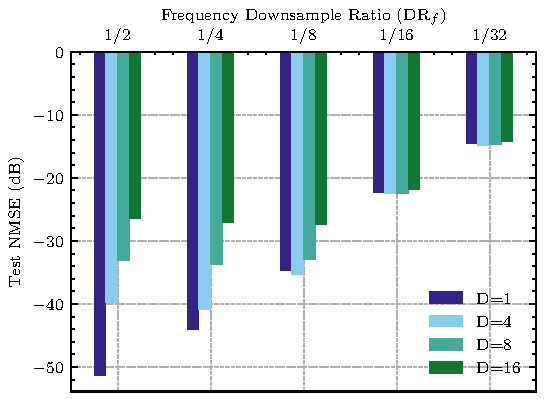
\includegraphics{./images/outdoor_p2d_diag.pdf}
    \caption{P2D estimation performance under different frequency downsampling ratios ($\text{DR}_f=\frac{M_f}{N_f}$) and diagonal dimensions ($D$) for the Outdoor COST2100 dataset. Downsampling is done along the frequency axis.}
    \label{fig:outdoor_p2d_init}
\end{figure}

We assess the accuracy of the P2DE assuming noise from pilot estimation. To simulate pilot estimation error, we use additive Gaussian noise,
\begin{align*}
    \hat{\mathbf{H}}_d &= \mathbf{H}_d + \mathbf{N}_d
\end{align*}
where the elements of $\mathbf{N}_d$, $\mathbf{N}_d(i,j) \sim \mathcal{N}(0, \sigma^2)$ for $i \in \left[1,2,\dots, N_b\right], j \in \left[1,2,\dots, M_f\right]$. To achieve different SNR values for $\hat{\mathbf{H}}_d$, we simply vary the noise variance $\sigma^2$, and we use the P2DE at different pilot estimation noise levels. Figure~\ref{fig:snr_sweep} shows the accuracy of the P2DE for different values of $\sigma^2$.

In addition to varying the pilots estimation SNR, we also showcase the effect of varying $\delta$ (i.e., the ODIR parameter as described in Appendix~\ref{appdx:odir}). We observe that $\delta$ helps the P2DE achieve better performance under both low-noise and noisy conditions, i.e.,

\begin{itemize}
    \item \textbf{Low-noise condition (SNR $\mathbf{=-20}$ dB)}: The P2DE goes from $-8$ dB to $-22$ dB for $\delta=0$ and $\delta=0.5$, respectively.
    \item \textbf{Noisy condition (SNR $\mathbf{\geq -10}$ dB)}: The P2DE goes from $-9$ dB to $-30$ dB for $\delta=0$ and $\delta=0.5$, respectively.
\end{itemize}

\begin{figure}[!hbtp]
    \centering
    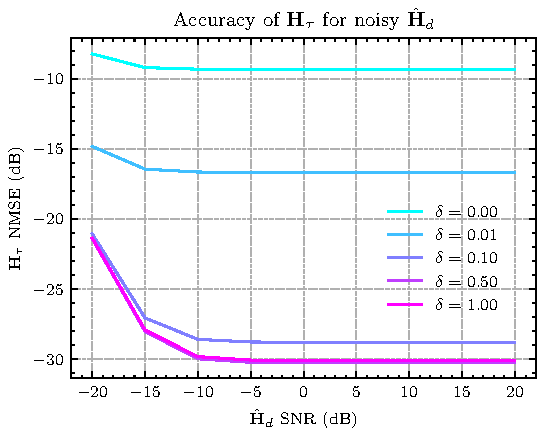
\includegraphics{outdoor_snr_sweep_delta_D4_sz32.pdf}
    \caption{Accuracy of P2DE output, $\mathbf{H}_{\tau}$, assuming noisy pilots, $\hat{\mathbf{H}}_d$. Additive Gaussian noise is used to model the error inherent in pilot estimation. Here, $D=4, \text{DR}_f=\frac{1}{32}$.}
    \label{fig:snr_sweep}
\end{figure}

\subsection{P2DE Compression Network Comparison}

Having assessed the initial accuracy of the P2DE at the UE, we now apply a deep learning network to compress the output of the P2DE. Figure~\ref{fig:outdoor_drcr_sweep} demonstrates the accuracy of ISTANet+ \cite{ref:zhang2018ista} for multiple compression ratios (CR) using the P2DE as its input. For progressively smaller compression ratios, the accuracy of ISTANet+ remains stable until $\text{DR}_f=\frac{1}{32}$, at which point the network's performance degrades.

\begin{figure}[!hbtp]
    \centering
    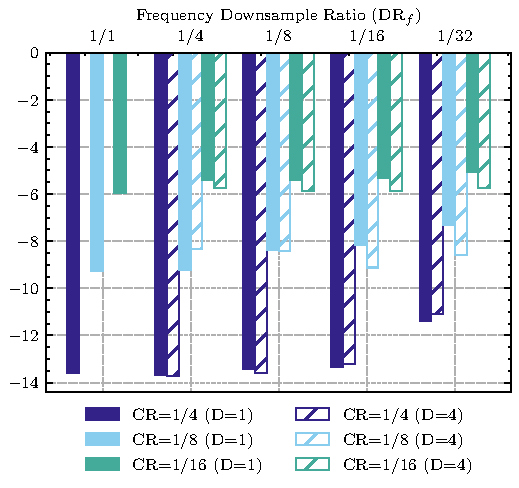
\includegraphics{./images/outdoor_drcr_D_sweep.pdf}
    \caption{Performance of ISTANet+ for multiple compression ratios using P2D estimates with different downsampling ratios ($\text{DR}_f=\frac{M_f}{N_f}$) for the Outdoor COST2100 dataset. Non-diagonal pattern ($D=1$) is compared with a diagonal pattern of size $D=4$. Performance for $\text{DR}_f=1/1$, $D=4$ is omitted since it is equivalent to the $\text{DR}_f=1, D=1$ case.}
    \label{fig:outdoor_drcr_sweep}
\end{figure}

In addition to ISTANet+, we assess the accuracy deep CNN autoencoders using P2DE as an input. Figure~\ref{fig:outdoor_net_ablation} shows the accuracy of ISTANet+ compared to ENet \cite{ref:Sun2021ENet} and SphNet \cite{ref:liu2020sphnet}. The performance of ISTANet+ is better than both ENet and SphNet at larger compression ratios ($\text{CR}\in [\frac 14, \frac 18]$), and the performance of ISTANet+ and ENet is comparable at $\text{CR}=\frac {1}{16}$.

\begin{figure}[!hbtp]
    \centering
    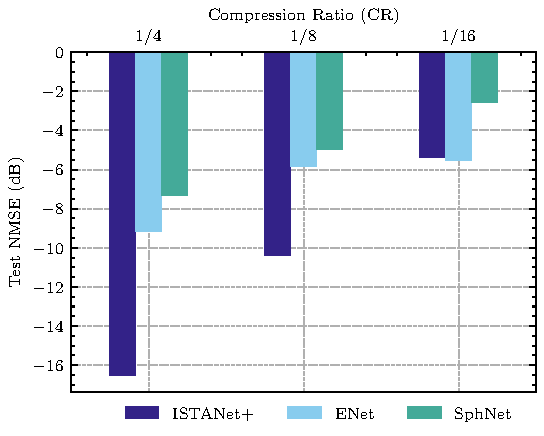
\includegraphics{outdoor_net_compare.pdf}
    \caption{Performance comparison for different feedback compression networks using P2D estimates ($\text{DF}_f=1/16, D=4$) for Outdoor COST2100 dataset. For all tested networks, we use $N_{\text{phase}}=4$, resulting in an augmented training set with $80$k samples.}
    \label{fig:outdoor_net_ablation}
\end{figure}

To assess the accuracy of these networks under quantization, we also conduct an experiment where the latent feedback elements are subjected to $\mu$-law companding and uniform quantization (as described in Section~\ref{sec:markov-results}). We present these results in Figure~\ref{fig:net_quant}.

\begin{figure}[!hbtp]
    \centering
    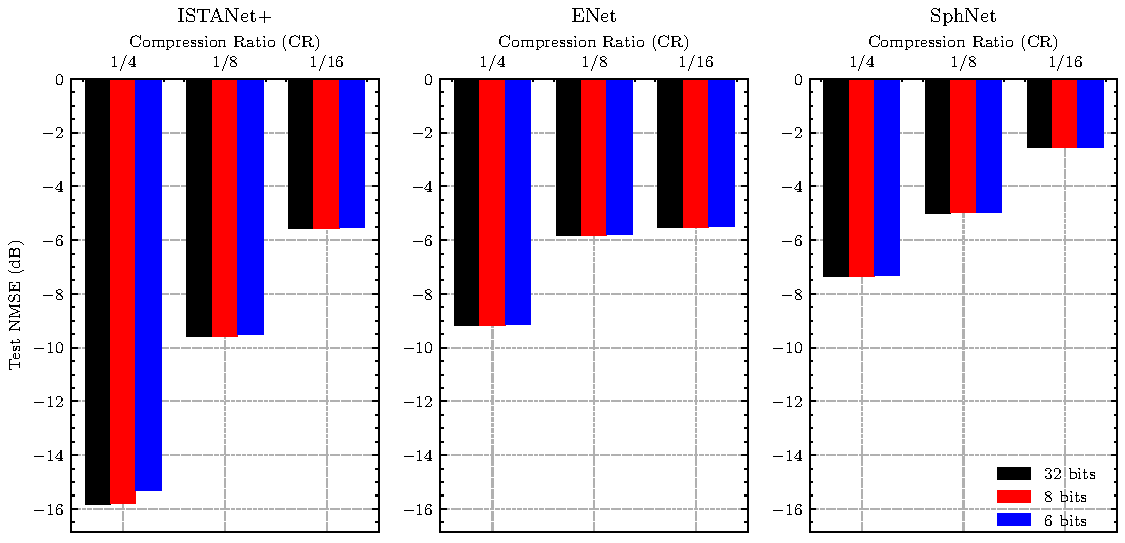
\includegraphics[width=\linewidth]{./images/outdoor_net_quant.pdf}
    \caption{Tested networks where feedback is subject to $\mu$-law companding ($\mu=255$) and uniform quantization for different numbers of quantization bits. P2DE parameters are $D=4, \text{DR}_f=\frac{1}{16}$.}
    \label{fig:net_quant}
\end{figure}

\subsection{Heterogeneous Differential Encoding Networks}

Figure~\ref{fig:markov-p2d-results} shows the performance of the proposed heterogeneous differential encoding networks compared to homogeneous networks. We observe that ENet provides worse initial performance than ISTANet+ (i.e., at $t_1$) but provides a more improvement in accuracy than ISTANet+ in subsequent timeslots (i.e., at $t_2, t_3, \dots$). Based on this observation, we expect the best network configuration to be the heterogeneous network, MN-IE. Figure~\ref{fig:markov-p2d-results} supports this reasoning, as MN-IE achieves better asymptotic performance (i.e., as $i$ for $t_i$ increases) than MN-I.

\begin{figure}[!hbtp]
    \centering
    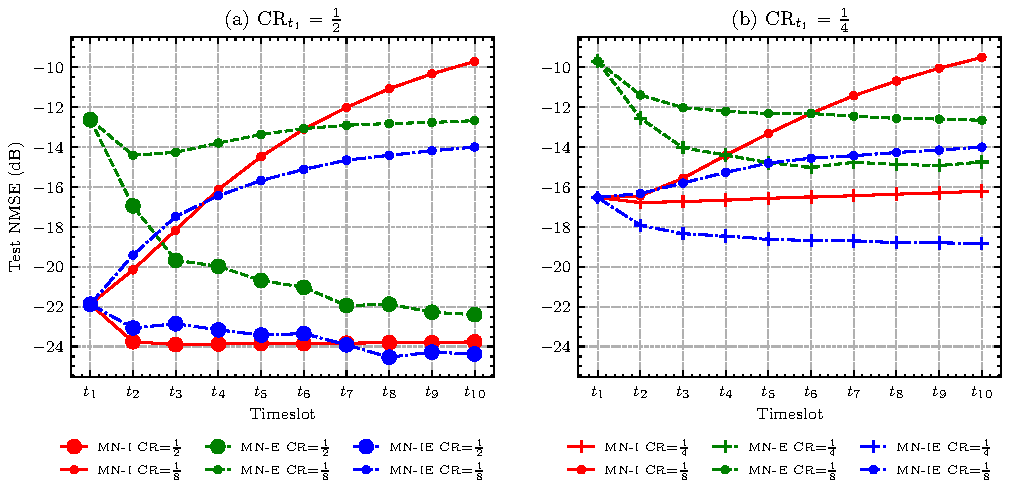
\includegraphics{outdoor_markov_sweep_v2.pdf}
    \caption{Compressive CSI estimation using differential encoding and  linear P2D estimator ($M_f=128, \text{DR}_f=\frac{1}{8}, D=4$). MarkovNet-ISTA (MN-I), MarkovNet-ENet (MN-E), and MarkovNet-ISTA-ENet (MN-IE) are tested using two different compression ratios in the first timeslot, $\text{CR}_{t_1}\in\left[\frac{1}{2},\frac{1}{4}\right]$.}
    \label{fig:markov-p2d-results}
\end{figure}

\subsection{Computational Complexity}

We assess the computational complexity (as defined in Chapter~\ref{chap:sph_norm}, Section~\ref{sect:dl_overview}) of the network architectures tested in this work. While ISTANet+ has superior accuracy compared to the autoencoder networks, we observe that its computational complexity is much higher. This discrepancy in complexity further motivates the heterogeneous network architecture of MN-IE. While MN-I uses $T$ copies of ISTANet+, MN-IE uses one copy of ISTANet+ to provide an initial estimate and $T-1$ copies of ENet to compress the differential term.

\begin{table}[htb]
\centering
\caption{Computational complexity of networks used in this work. \textbf{Bold face} in a column indicates lowest value for given compression ratio. ``CR" $=$ compression ratio, ``Enc" $=$ encoder, ``Dec" $=$ decoder. FLOPs indicate computation during inference (i.e., not training/back-propagation).}
\label{tab:net-complexity} 

\begin{tabular}{|cc|cccc|cc|}
\hline
\multicolumn{2}{|c|}{\multirow{2}{*}{}}                    & \multicolumn{4}{c|}{Parameters (M)}                                                                                          & \multicolumn{2}{c|}{\multirow{2}{*}{FLOPs (M)}}     \\ \cline{3-6}
\multicolumn{2}{|c|}{}                                     & \multicolumn{2}{c|}{Trainable}                                          & \multicolumn{2}{c|}{All}                           & \multicolumn{2}{c|}{}                               \\ \hline
\multicolumn{1}{|c|}{}                            & CR     & \multicolumn{1}{c|}{Enc}           & \multicolumn{1}{c|}{Dec}           & \multicolumn{1}{c|}{Enc}           & Dec           & \multicolumn{1}{c|}{Enc}           & Dec            \\ \hline
\multicolumn{1}{|c|}{\multirow{4}{*}{ISTANet+}}    & $1/2$  & \multicolumn{1}{c|}{\textbf{0.00}} & \multicolumn{1}{c|}{\textbf{0.34}} & \multicolumn{1}{c|}{2.10}          & 4.54          & \multicolumn{1}{c|}{\textbf{2.10}} & 393.78         \\ \cline{2-8} 
\multicolumn{1}{|c|}{}                            & $1/4$  & \multicolumn{1}{c|}{\textbf{0.00}} & \multicolumn{1}{c|}{0.34}          & \multicolumn{1}{c|}{1.05}          & 2.44          & \multicolumn{1}{c|}{\textbf{1.05}} & 373.85         \\ \cline{2-8} 
\multicolumn{1}{|c|}{}                            & $1/8$  & \multicolumn{1}{c|}{\textbf{0.00}} & \multicolumn{1}{c|}{0.34}          & \multicolumn{1}{c|}{0.52}          & 1.39          & \multicolumn{1}{c|}{\textbf{0.52}} & 363.89         \\ \cline{2-8} 
\multicolumn{1}{|c|}{}                            & $1/16$ & \multicolumn{1}{c|}{\textbf{0.00}} & \multicolumn{1}{c|}{0.34}          & \multicolumn{1}{c|}{0.26}          & 0.87          & \multicolumn{1}{c|}{\textbf{0.26}} & 358.91         \\ \hline
\multicolumn{1}{|c|}{\multirow{4}{*}{ENet}}       & $1/2$  & \multicolumn{1}{c|}{0.55}          & \multicolumn{1}{c|}{0.55}          & \multicolumn{1}{c|}{\textbf{0.55}} & \textbf{0.55} & \multicolumn{1}{c|}{29.98}         & 29.70          \\ \cline{2-8} 
\multicolumn{1}{|c|}{}                            & $1/4$  & \multicolumn{1}{c|}{0.29}          & \multicolumn{1}{c|}{\textbf{0.29}} & \multicolumn{1}{c|}{\textbf{0.29}} & \textbf{0.29} & \multicolumn{1}{c|}{29.46}         & 29.18          \\ \cline{2-8} 
\multicolumn{1}{|c|}{}                            & $1/8$  & \multicolumn{1}{c|}{0.16}          & \multicolumn{1}{c|}{\textbf{0.16}} & \multicolumn{1}{c|}{\textbf{0.16}} & \textbf{0.16} & \multicolumn{1}{c|}{29.20}         & 28.92          \\ \cline{2-8} 
\multicolumn{1}{|c|}{}                            & $1/16$ & \multicolumn{1}{c|}{0.09}          & \multicolumn{1}{c|}{\textbf{0.09}} & \multicolumn{1}{c|}{\textbf{0.09}} & \textbf{0.09} & \multicolumn{1}{c|}{29.07}         & 28.79          \\ \hline
\multicolumn{1}{|c|}{\multirow{4}{*}{CsiNet Pro}} & $1/2$  & \multicolumn{1}{c|}{1.06}          & \multicolumn{1}{c|}{1.06}          & \multicolumn{1}{c|}{1.06}          & 1.06          & \multicolumn{1}{c|}{12.16}         & \textbf{12.16} \\ \cline{2-8} 
\multicolumn{1}{|c|}{}                            & $1/4$  & \multicolumn{1}{c|}{0.53}          & \multicolumn{1}{c|}{0.53}          & \multicolumn{1}{c|}{0.53}          & 0.53          & \multicolumn{1}{c|}{11.11}         & \textbf{11.11} \\ \cline{2-8} 
\multicolumn{1}{|c|}{}                            & $1/8$  & \multicolumn{1}{c|}{0.27}          & \multicolumn{1}{c|}{0.27}          & \multicolumn{1}{c|}{0.27}          & 0.27          & \multicolumn{1}{c|}{10.59}         & \textbf{10.59} \\ \cline{2-8} 
\multicolumn{1}{|c|}{}                            & $1/16$ & \multicolumn{1}{c|}{0.14}          & \multicolumn{1}{c|}{0.14}          & \multicolumn{1}{c|}{0.14}          & 0.14          & \multicolumn{1}{c|}{10.33}         & \textbf{10.33} \\ \hline
\end{tabular}
\end{table}

\chapter{Improving Computational Efficiency} \label{chap:comp-effic}

The prior works discussed in this dissertation have leveraged domain knowledge to improve the performance of deep neural networks for CSI compression. In this chapter, we consider some methods for improving the efficiency of such networks.

In Chapter~\ref{chap:p2d}, we considered how to use frequency domain pilots at the UE to estimate the truncated delay domain. While it is advantageous to acquire the delay domain CSI at the UE from a sparsity perspective, utilizing the P2DE at the UE creates additional computational and memory burden. Consider the P2DE estimator as outlined in Algorithm~\ref{alg:p2d-diag}. The algorithm iterates over the $N_b$ antennas and performs the matrix multiplication $\eta_{d,i}\mathbf{Q}_{c,j}^{\#}$ in each iteration. To run the algorithm, $N_bM_f(N_f-1)$ FLOPs are required\footnote{Considering the $M_f(N_f-1)$ FLOPs involved in matrix multiplication (as discussed in Appendix~\ref{appdx:complexity-linear}), and considering that this matrix multiplication occurs $N_b$ times.}, and $2D(M_fN_f)$ parameters must be stored\footnote{Considering the matrices $\mathbf{Q}_i^{\#} \in \mathbb{C}^{M_f \times N_f}$ for $i \in [1, \dots, D]$.}. Under the parameters used in Chapter~\ref{chap:p2d} Section~\ref{sect:p2de-results}, utilizing the P2DE at the UE could result in an additional $1.04\times 10^{6}$ FLOPs and $2.62\times 10^{5}$ parameters. The additional computational burden of the P2DE is summarized in Table~\ref{tab:p2de-comp}. % 32*32*(1024-1) 1047552 FLOPs, 2*4*32*1024=262144

\begin{table}[!h]
\caption{Computational complexity of P2DE for $D=1$ (diagonal pattern size), $N_f=1024$ (number of subcarriers), and $N_b=32$ (number of antennas in uniform linear array).}
\begin{center}
\label{tab:p2de-comp} 
\begin{tabular}{|r|c|c|c|}
\hline
$\mathbf{M_f}$      & $\mathbf{32}$      & $\mathbf{64}$       & $\mathbf{128}$     \\ \hline
\textbf{FLOPs}      & $1.05\cdot 10^{6}$ & $2.10\cdot 10^{6}$  & $4.19\cdot 10^{6}$ \\ \hline
\textbf{Parameters} & $6.55\cdot 10^{4}$ & $1.31\cdot 10^{5}$  & $2.62\cdot 10^{5}$  \\ \hline
\end{tabular}
\end{center}
\vspace*{-0.3mm}
\end{table}

Since UEs are typically compute/memory constrained devices (e.g., cell phones, tablets, IoT devices), it is preferable to reduce any such burden where possible. In this chapter, we propose two methods to reduce computational complexity at the UE. In Section~\ref{sect:direct_pilots}, we propose a method to estimate the delay domain CSI at the BS based on compressed feedback of the frequency domain pilots. In Section~\ref{sect:model_reuse}, we propose a method for using a simple model to estimate subsets of subcarriers in CSI matrices. In Section~\ref{sect:direct_reuse_results}, we present results demonstrating that these methods maintain CSI estimation accuracy while reducing encoder-side complexity by as much as a factor of 10. 

\section{Direct Pilot-based Feedback} \label{sect:direct_pilots}

\begin{figure}[!hbtp]
    \centering
    {
      \fontsize{8pt}{8pt}
      \def\svgwidth{1.0\linewidth}
      \input{./images/01_downlink_p2d_direct_feedback_horiz_diag.pdf_tex}
    }
    % \input{figure/csinet_quant.pdf_tex}
    \caption{Compressive CSI estimation based on linear P2D estimator on BS side. First,
    we use downlink pilots to 
    generate a sparse, frequency domain CSI
    estimate 
    of size $M_f << N_f$. This downsampled frequency domain CSI estimate is compressed at the UE
    and fed back to the BS.
    At the BS, we apply
    the P2D estimator, $\mathbf{Q}^{\#}_{N_t}$ \cite{ref:delRosario2022p2d} to acquire 
    the truncated
    delay domain CSI estimate.
    We train a
    learnable encoder, 
    $f(x)$,
    and decoder, $g(x)$, to compress and decode the feedback, respectively. The 
    BS recovers
    the frequency domain
    CSI from 
    the decoded 
    delay domain CSI estimate.}
    \label{fig:p2d_direct}
\end{figure}

Many works in deep learning based compressive CSI estimation 
have leveraged delay domain CSI given its sparsity \cite{ref:csinet}.
Recent work has confirmed the viability of acquiring the truncated delay domain 
at the UE under realistic conditions (i.e., using sparse frequency-domain pilots) \cite{ref:delRosario2022p2d}.

However, the process of acquiring delay domain CSI places additional 
computational burden on the UE, and given the computational constraints
of typical UEs (e.g., cell phones, tablets, IoT devices), minimizing the 
computational burden on the UE should be prioritized.

To reduce the computation performed at the UE, we propose to move the computation of 
the delay domain to the BS by compressing and feeding back the frequency domain pilots.
The data flow of this scheme is illustrated in Fig~\ref{fig:p2d_direct}, where the 
P2DE (see \cite{ref:delRosario2022p2d} for full details) is utilized at the 
BS rather than the UE.

\section{Model Re-use} \label{sect:model_reuse}

In order to enjoy the benefits of highly accurate CS networks while
reducing network complexity at the UE, we propose to use a relatively simple CS
model on contiguous blocks of $K$ subcarriers where $K \leq M_f$.
The operating principle behind this approach is inspired by block 
compressed sensing \cite{ref:Gan2007blockCS}, and the concept is 
shown in Fig.~\ref{fig:model_reuse}.

In this work, we study a deep CS network called ISTANet+ \cite{ref:zhang2018ista}.
For ISTANet+, the compression occurs at the UE by a simple matrix multiplication, 
\begin{align}
    f(x) &= \mathbf{\Phi}\mathbf{x}
\end{align}
where $\mathbf{\Phi}$ is referred to as the measurement matrix and 
$\mathbf{x}$ is the flattened CSI matrix. In the case of block compressed
sensing, the measurement matrix operates of $K$ contiguous subcarriers across
all angular indices, i.e., $\mathbf{x} \in \mathbb{R}^{N_K}$, $\mathbf{\Phi} 
\in \mathbb{R}^{\text{CR} K  \times K}$ where $N_K = 2 K N_a$ is the dimension of
the $K$ subcarriers from the CSI matrix. The decoder of ISTANet+ is identical 
to the original paper, the only major differnce being the dimension of the latent
2D convolutions to accommodate $K$ subcarriers rather than all $M_f$ pilot subcarriers.

To produce a full CSI estimate at the BS, the encoder is run $\frac{M_f}{K}$ times
on adjacent blocks of subcarriers, producing multiple feedback payloads. At the BS, 
each of these payloads is decoded to estimate a block of subcarriers, and the final CSI
estimate is simply the concatenation of all these decoded payloads.

\begin{figure}
    \centering
    {
      \fontsize{8pt}{8pt}
      \def\svgwidth{1.0\linewidth}
      \input{./images/02_per_K_subc.pdf_tex}
    }
    \caption{Compressive CSI estimation with model re-
    use. Rather than compressing the entire input, $\mathbf{H}_d$,
    the encoder compresses $K$ contiguous subcarriers
    from the input, resulting in $\frac{M_f}{K}$ payloads of feedback
    (shown in different colors above). Meanwhile at the
    BS, the decoder recovers each set of $K$ contiguous
    subcarriers based on the $\frac{M_f}{K}$ payloads, and the
    decoded payloads are combined to generate the full
    frequency domain estimate.}
    \label{fig:model_reuse}
\end{figure}

\section{Results} \label{sect:direct_reuse_results}

To evaluate the effectiveness of direct frequency-domain CSI feedback and of model re-use, we use CSI data generated by the COST2100 model in an Indoor and an Outdoor scenario \cite{ref:liu2012cost2100}. The parameters used to generate both datasets are given at the end of Chapter~\ref{chap:intro} Section~\ref{sect:channel_model}. For all tests, we utilize ISTANet+ with spherical normalization \cite{ref:liu2020sphnet}.% Importantly, we utilize a relatively small number of channel samples when compared to similar works, as we store full CSI matrices without truncating any subcarriers, which requires 32 times more space to store. 

\subsection{Accuracy vs. $K$ Subcarriers} \label{sect:acc_vs_k}

Figures~\ref{fig:outdoor_nmse_vs_K} and~\ref{fig:indoor_nmse_vs_K} compare the reused models with frequency domain compression against the original delay domain model (shown in {\color{red}red} in both Figures). We test the networks using $K\in [2,4,8,16,32,64,128]$ with the requirement that $K < M_f$. We observe that in the Indoor network, there is a gradual increase in NMSE as the number of subcarriers reduces. In the case of the Outdoor network, the frequency domain-based feedback results in a drop in NMSE by about 2.5 dB.

\begin{figure}[!hbtp]
    \centering
    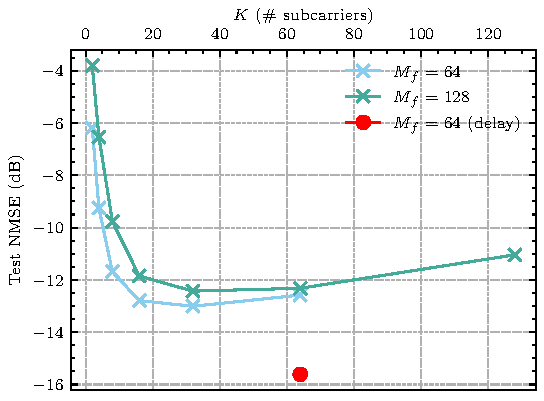
\includegraphics{outdoor_K_subc_sweep.pdf}
    \caption{NMSE vs. $K$ subcarriers of shared model architectures (i.e., complexity is w.r.t. FLOPs and parameters at UE). Outdoor COST2100 model.}
    \label{fig:outdoor_nmse_vs_K}
\end{figure}

\begin{figure}[!hbtp]
    \centering
    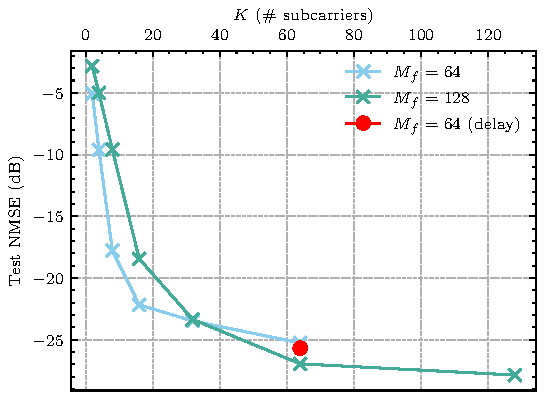
\includegraphics{indoor_K_subc_sweep.pdf}
    \caption{NMSE vs. $K$ subcarriers for shared model architectures (i.e., complexity is w.r.t. FLOPs and parameters at UE). Indoor COST2100 model.}
    \label{fig:indoor_nmse_vs_K}
\end{figure}

\subsection{Accuracy vs. Network Complexity} \label{sect:acc_vs_comp}

In Figures~\ref{fig:outdoor_nmse_vs_complexity} and~\ref{fig:indoor_nmse_vs_complexity}, we compare the reused models with frequency domain compression against the original model with delay domain compression (shown in {\color{red}red} in both Figures). Both Figures show the performance of the given model vs. a complexity metric, either log(FLOPs) or the number of model parameters. The complexity of the model varies with $K$, which we vary in the same way as described above in Section~\ref{sect:acc_vs_k}. Importantly, each complexity metric is given for the \emph{encoder} (i.e., the UE-side complexity).

\begin{figure}[!hbtp]
    \centering
    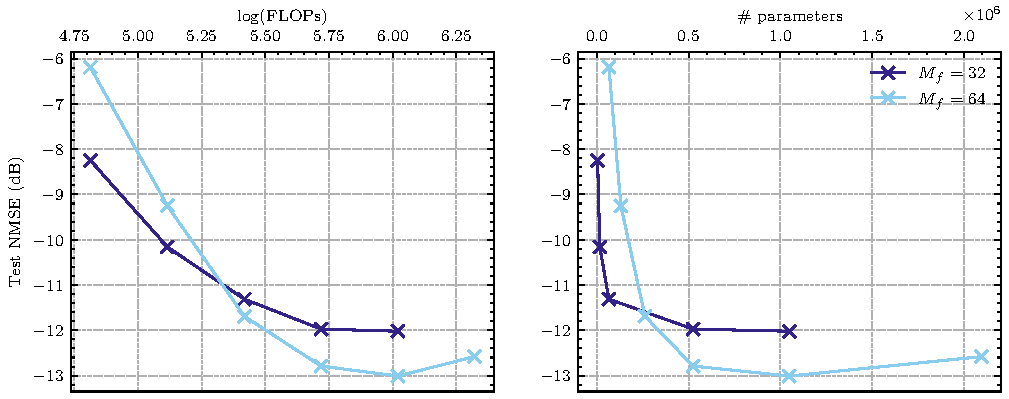
\includegraphics{outdoor_subc_sweep_line.pdf}
    \caption{NMSE vs. encoder complexity of shared model architectures (i.e., complexity is w.r.t. FLOPs and parameters at UE). Outdoor COST2100 model.}
    \label{fig:outdoor_nmse_vs_complexity}
\end{figure}

\begin{figure}[!hbtp]
    \centering
    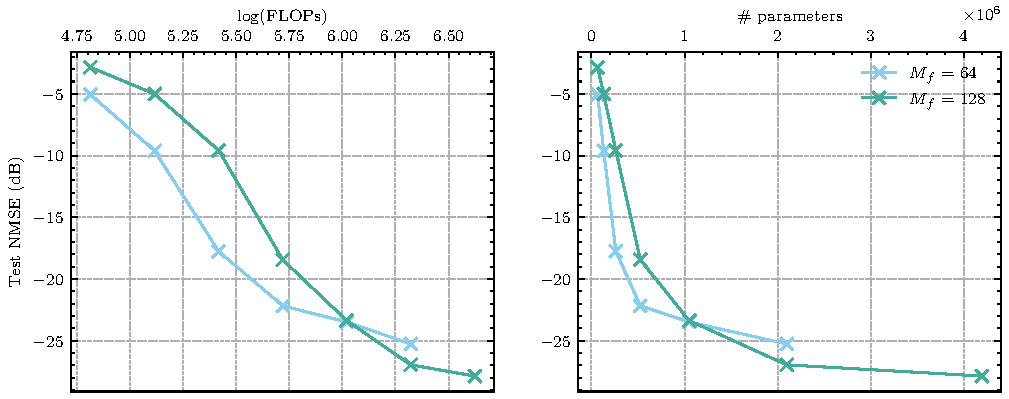
\includegraphics{indoor_subc_sweep_line.pdf}
    \caption{NMSE vs. encoder complexity for shared model architectures (i.e., complexity is w.r.t. FLOPs and parameters at UE). Indoor COST2100 model.}
    \label{fig:indoor_nmse_vs_complexity}
\end{figure}

Figures~\ref{fig:outdoor_nmse_vs_complexity_w_dec} and~\ref{fig:indoor_nmse_vs_complexity_w_dec} show the same performance and complexity metrics as Figures~\ref{fig:outdoor_nmse_vs_complexity} and~\ref{fig:indoor_nmse_vs_complexity} but with respect to the full model complexity (i.e., encoder and decoder, UE-side and BS-side). When it comes to parameters, we observe trends that are similar to the encoder-side parameters in both environments. However, the number of FLOPs for the $M_f=128$ case is twice that of the the $M_f=64$ case since the number of FLOPs of the decoder scales linearly with $M_f$.

\begin{figure}[!hbtp]
    \centering
    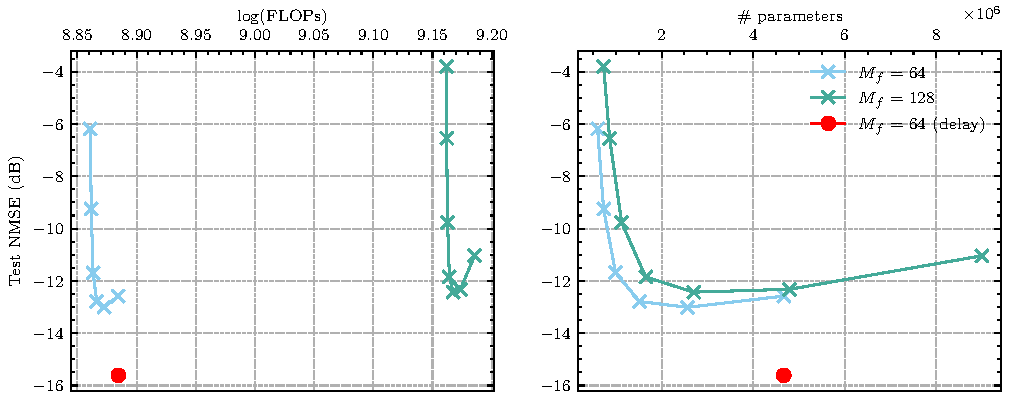
\includegraphics{outdoor_subc_sweep_line_w_dec.pdf}
    \caption{NMSE vs. complexity of shared model architectures. \textbf{Left}: Complexity w.r.t. FLOPs of encoder and decoder. \textbf{Right}: Complexity w.r.t. parameters of encoder and decoder.). Outdoor COST2100 model.}
    \label{fig:outdoor_nmse_vs_complexity_w_dec}
\end{figure}

\begin{figure}[!hbtp]
    \centering
    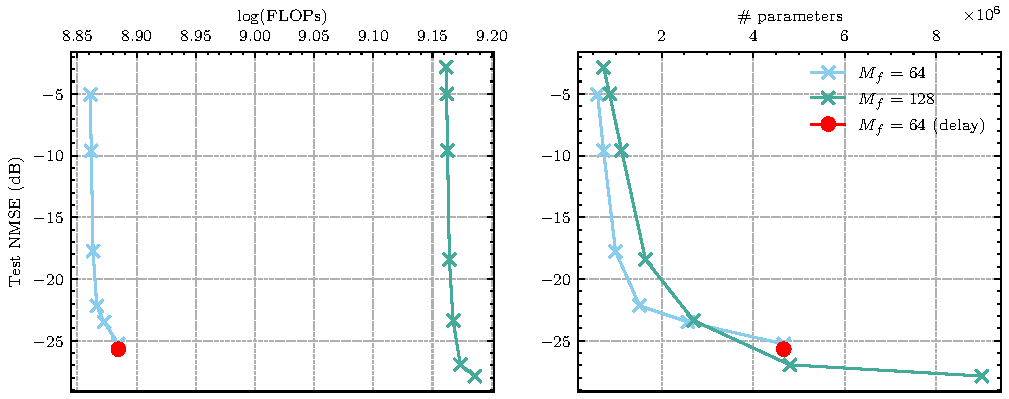
\includegraphics{indoor_subc_sweep_line_w_dec.pdf}
    \caption{NMSE vs. complexity for shared model architectures. \textbf{Left}: Complexity w.r.t. FLOPs of encoder and decoder. \textbf{Right}: Complexity w.r.t. parameters of encoder and decoder.). Indoor COST2100 model.}
    \label{fig:indoor_nmse_vs_complexity_w_dec}
\end{figure}

\section{Discussion}

In this chapter, we presented two methods for reducing the complexity of deep learning based CSI compression networks. We first proposed to move the delay domain estimation to the BS by compressing and feeding back frequency domain information to directly estimate the pilots at the UE. We then proposed to use a deep learning model to estimate blocks of $K$ contiguous subcarriers. We tested a combination of both of these approaches in both the Indoor and Outdoor COST2100 scenarios, and we demonstrated that these approaches can reduce the UE-side computational complexity while maintaining or slightly increasing the network's final accuracy.
\chapter{Conclusion} \label{chap:conclusion}

This dissertation investigates techniques to improve the performance and efficiency of deep neural networks for the task of MIMO CSI estimation. In Chapter~\ref{chap:sph_norm} we discussed the importance of data pre-processing techniques, and we showed the efficacy of our proposed spherical normalization technique. In Chapter~\ref{chap:markovnet}, we exploited the temporal correlation of the wireless channel, and we demonstrated the superior performance and efficiency of a deep differential encoder compared to recurrent neural networks. In Chapter~\ref{chap:p2d}, we presented two main contributions: an accurate estimator of the delay domain CSI based on sparse frequency domain pilots and a hetergeneous differential encoding network combining deep compressive sensing networks with autoencoders. We showed the accuracy of our pilot-based delay domain estimator, even under aggressive sparsity and noisy pilot estimates. Furthermore, we verified the improved performance of heterogeneous networks over homogeneous networks. Finally in Chapter~\ref{chap:comp-effic}, we proposed a scheme which re-uses a simple model on contiguous blocks of multiple subcarriers, and we showed that this method can maintain accuracy while reducing the computational complexity of the network by a factor of 10.  

Across all these works, we investigated techniques which exploited domain knowledge of the wireless channel to improve estimation accuracy and computational efficiency while better conforming to 3GPP protocols. Further work in CSI compression should take a similar approach by taking advantage of features of the wireless channel, the communications protocol, or CSI data itself.

\section{Future Works}

In addition to the work discussed in this dissertation, there are important additional directions which future works in deep learning for CSI compression should address. Here, we discuss a few such directions, including compression bounds for CSI estimation, networks with trainable codewords, and ...  

\subsection{Rate-distortion Bounds for CSI Feedback}

Many works provide results for their proposed CSI feedback networks using the NMSE at a small number of compression ratios. This approach allows for fair comparison between comparable networks/algorithms, but it does not answer a more important question: \emph{At a given compression ratio, what is the theoretical distortion limit?}

Information theory provides us with a framework to answer this question: the rate-distortion curve. The rate-distortion of a random variable describes the optimal error that can be achieved whenever that variable is encoded using a given number of bits.

The challenge with applying rate-distortion theory to MIMO CSI data is the lack of well-defined distributions for practical channel data. While rate-distortion bounds are known for well-defined distributions (e.g., univariate or multivariate Gaussian distributions), the same can not be said for empirical data.

One possible approach to constructing a rate-distortion curve is to estimate the differential entropy of quantized CSI data. For a CSI matrix, $\mathbf{H}$, assume i.i.d. $\mathbf H_{(i,j)}$ where $i$ ($j$) denotes the row (column) of $\mathbf{H}$. The differential entropy of the $(i,j)$-th element is
\begin{align*}
	h(\mathbf H_{(i,j)}) &= - \int p(\mathbf H{(i,j)} = k) \log p(\mathbf H_{(i,j)} = k) dk,
\end{align*}
In practice, the distribution $p(\mathbf H_{(i,j)})$ is difficult to obtain. We can instead resort to the Kozachenko–Leonenko (KL) estimator \cite{ref:Kozachenko1987SampleEstimate} for each element in $\mathbf H$ and average over the elements,
\begin{align}
	h(\mathbf H) &\leq \sum_{i}^{R_d}\sum_{j}^{n_T} \hat h(\mathbf H_{(i,j)}) = h_{\text{UB}}(\mathbf H), \label{eq:csi-diff-ent}
\end{align}
for KL estimator $\hat h$. Based on Theorem 8.3.1 from Cover \cite{ref:Cover1999Elements}, for sufficiently small quantization interval $\Delta = \frac {1}{2^n}$, the entropy of a quantized random variable is related to its differential entropy as,
\begin{align}
  H(\mathbf H^{\Delta}) &= h(\mathbf H) + n, \label{eq:cover-thm}
\end{align}
for $n$-bit quantization. Thus, the differential entropy estimator admits an estimate for the entropy of the quantized CSI, $\hat H({\mathbf H}^\Delta) = \hat h(\mathbf H) + n$.

To establish a rate-distortion curve, we can use the estimator outlined above on CSI data with Gaussian noise, i.e.
\begin{align*}
	\mathbf H_{\sigma,(i,j)} &= \mathbf H_{(i,j)} + v \text{ for i.i.d } v \sim \mathcal{N}(0,\sigma^2).
\end{align*}
Using the corrupted CSI matrices $\mathbf H_{\sigma}=\left[\mathbf H_{\sigma,(i,j)}\right]_{i\in [R_d],j\in [N_b]}$, we calculate the bounds $\hat h(\mathbf H_{\sigma}^\Delta)$ from or (\ref{eq:csi-diff-ent}) for different noise levels $\sigma$ to establish a rate-distortion curve.

\subsection{Trainable Codewords}

In addition to estimating the rate-distortion bounds of CSI data, new works should investigate techniques for improving the compression efficiency of CSI feedback networks. Some prior work has investigated feedback quantization in deep learning-based CSI compression. In \cite{ref:Yang2019DeepCMC}, the authors propose DeepCMC, an autoencoder structure where the continuous compressed elements are discretized via uniform quantization then encoded using context adaptive binary arithmetic coding (CABAC) \cite{ref:Marpe2003CABAC}. Since uniform quantization is non-differentiable, the authors do not perform true quantization during training and instead apply uniformly distributed noise to approximate quantization noise \cite{ref:Yang2019DeepCMC}. In \cite{ref:Mashhadi2020AnalogDeepCMC}, the authors propose AnalogDeepCMC, which encodes latent elements as power-normalized complex elements and decodes using maximal ratio combining. The authors also report the achieved rate of AnalogDeepCMC for different CSI overhead ratios.

Further work into trainable codewords might borrow ideas from deep learning based image compression. For example, the soft-to-hard vector quantization (SHVQ) framework \cite{ref:Agustsson2017SoftToHard} could be used to imbue a CSI compression network with quantized codewords. To describe the framework, we choose a vector dimension, $m$, by which to partition the latent space $\mathbf Z = f_e(\mathbf H, \theta_e)$, and we denote the vectorized version of $\mathbf Z \in \mathbb R^{r}$ as $\tilde{\mathbf Z} \in \mathbb R^{r/m \times m}$. We define the $m$-dimensional codebook of size $L$ as $\mathbf C \in \mathbb R^{m\times L}$. The soft assignments of the $j$-th latent vector $\tilde{\mathbf z}_j$ can be written as
\begin{align}
\phi(\tilde{\mathbf z}_j) &= \left[\frac{\text{exp}(-\sigma \Arrowvert \tilde{\mathbf z}_j - \mathbf c_\ell\Arrowvert^2)}{\sum_{i=1}^L\text{exp}(-\sigma \Arrowvert \tilde{\mathbf z}_j - \mathbf c_i\Arrowvert^2)}\right]_{\ell\in [L]} \in \mathbb R^L \label{eq:soft_assign}
\end{align}
where (\ref{eq:soft_assign}) is typically referred to as the \emph{softmax} function, a differentiable alternative to the max function. The hyperparameter $\sigma$ controls the temperature of the softmax scores, with a lower $\sigma$ yielding a more uniform distribution and a higher $\sigma$ yielding a ``peakier'' distribution (i.e., $\sigma \to \infty \Rightarrow \phi(\tilde z_j) \to \text{max}(\tilde z_j)$). Using the soft assignments, the latent vectors are quantized based on the codebook $\mathbf C \in \mathbb R^{m \times L}$,
\begin{align}
Q(\tilde{\mathbf z}_j,\mathbf C) &= \phi(\tilde{\mathbf z}_j) \mathbf C^T. \label{eq:soft_quant}
\end{align}
The quantized version of the latent vector is taken by reshaping $\mathbf Q(\tilde{\mathbf Z},\mathbf C) \in \mathbb R^{r/m \times m}$ into $\hat{\mathbf Z} \in \mathbb R^d$, and the decoder produces the CSI estimates as $\hat{\mathbf H} = h(\hat{\mathbf Z}, \mathbf C)$. An abstract illustration of an autoencoder using soft quantization can be seen in Figure~\ref{fig:csinet_quant}.

\begin{figure*}[!hbtp]
\centering
\def\svgwidth{0.8\linewidth}
\input{images/csinet_quant.pdf_tex}
\caption{Abstract architecture for a CSI compression network with the `SoftQuantize' layer ($Q(\tilde{\mathbf Z})$), a continuous, softmax-based relaxation of a $d$-dimensional quantization of the latent layer $\mathbf Z$.}
\label{fig:csinet_quant}
\end{figure*}
% \chapter{Conclusions}
\label{chap:conclusion}

We have explored non-convex optimization in the context of wireless communications under geometrical perspectives, using new techniques developed for seemingly unrelated problems. We have also proposed new geometrical perspectives for both grant-free access and grant-free scheduling, leveraging the underlying properties of the computational space to improve the performance of these tasks with reasonable computational complexity and minimal ad-hoc settings.

% WF-CMA
\section{CMA via Wirtinger Flow}
First, we used known results and algorithms for phase retrieval and applied this knowledge into the blind beamforming problem. We generalized the convergence analysis of WF for our WF-CMA algorithm by incorporating new conditions of subgaussian signal sources and average modulus, demonstrating its global convergence for blind signal recovery with high probability under limited data samples. 
We characterized the local geometry of the CM cost function in terms of smoothness and convexity, which enables parameter updates to remain within the basin of attraction for a defined stepsize. This allows to establish a more aggressive stepsize than the traditional gradient-descent CMA approaches, tackling the slow convergence of the latter with no significant increase in the computational cost.  


% RMSR
\section{Riemannian Multiple Signal Recovery}
We also developed a Riemannian framework for blind source recovery problems, and to the best of our knowledge, is the first work using these techniques for CMA-based formulations.
This is achieved by means of minimizing a CMA cost function, such that the orthogonality of different demixers is embedded in the geometry of a Riemannian manifold. We derive this geometry and obtain the geometrical definitions that allow to minimize over the manifold as the search space of the optimization problem. The results of our approach show high probability of successful recovery of all sources with a reasonable number of samples, for rather large system sizes and different modulation schemes. 


% U-SCH
\section{Unsupervised Riemannian User Scheduling}
Last but not least, we focused on the uplink user scheduling problem that exploits spatial multiplexing in MIMO systems. To mitigate the intra-group interference, instead of directly scheduling users with high channel dissimilarity, we developed a general uplink user scheduling strategy that selects users from different high-similarity channel clusters, by exploiting unsupervised learning algorithms without the requirement of a significant number of labeled data. We identified a Riemannian manifold that inherently describes the similarity of channels with respect to their cross-correlation, which is invariant to both phase and magnitude differences. Using this manifold as the underlying computational space, we exploit the retrieved similarity information to assist in the scheduling of users.
Under a variety of performance metrics to evaluate user scheduling, simulations indicate that the combination of a learning-enabled channel clustering can exploit the spatial compatibility effectively to reduce inter-group interference when compared with other benchmarks. 




\cleardoublepage
\phantomsection
%\addcontentsline{toc}{section}{References}
\addcontentsline{toc}{chapter}{References}
\bibliographystyle{IEEEtran}
\bibliography{cited_works}

\singlespacing
\appendix
\chapter{Computational Complexity of Common Layers}
\label{appdx:complexity}
Based on the measures of computational complexity in Chapter~\ref{chap:sph_norm} Section~\ref{sect:dl_overview}, i.e. FLOPs and parameters, we provide the corresponding formulas for common layers and operations used in the networks described in this dissertation. Note that any arithmetic operation (e.g., addition, multiplication) or non-linearity consumes a single FLOP, and certain non-linearities require a single parameter (e.g., the negative slope of a Leaky ReLU).

\section{Matrix Multiplication} \label{appdx:complexity-matmul}

Denote two matrices $\mathbf{A} \in \mathbb{R}^{M \times P}$ and $\mathbf{B} \in \mathbb{R}^{P \times N}$. Matrix multiplication between $\mathbf{A}$ and $\mathbf{B}$ is denoted as
\begin{align*}
	\mathbf{C} &= \mathbf{A}\mathbf{B} \in \mathbb{R}^{M\times N}, \; c_{ij} = \sum_{k=1}^P a_{ik}b_{kj} \; \forall \; i\in [1,\dots,M], i\in [1,\dots,N].
\end{align*}
\textbf{FLOPs}: Each element in $\mathbf{C}$ involves $P$ multiplications and $P-1$ additions, and $\mathbf{C}$ includes $M \times N$ elements. Thus, the amount of FLOPs involved in matrix multiplication is
\begin{align*}
	\text{FLOPs}_{\text{matmul}} &= (2P-1)MN
\end{align*}

\textbf{Parameters}: The number of `parameters' in matrix multiplicatiion depends on which matrix is considered the parameter matrix. If $\mathbf{A}$ is the parameter matrix, then the number of parameters is
\begin{align*}
	P_{\text{matmul}} &= MP.
\end{align*}
Alternatively, if $\mathbf{B}$ is the parameter matrix, then the number of parameters is
\begin{align*}
	P_{\text{matmul}} &= PN.
\end{align*}

\section{Complex Matrix Multiplication}  \label{appdx:complexity-matmul-comp}

Denote two complex matrices $\mathbf{A} \in \mathbb{C}^{M \times P}$ and $\mathbf{B} \in \mathbb{C}^{P \times N}$. Complex matrix multiplication between $\mathbf{A}$ and $\mathbf{B}$ is denoted as
\begin{align*}
	\mathbf{C} &= \mathbf{A}\mathbf{B} \in \mathbb{R}^{M\times N},\\ \; c_{ij} &= \sum_{k=1}^P [\text{Re}(a_{ik})\text{Re}(b_{kj}) - \text{Im}(a_{ik})\text{Im}(b_{kj})] \\ &\phantom{\sum} + j[\text{Re}(a_{ik})\text{Im}(b_{kj}) + \text{Im}(a_{ik})\text{Re}(b_{kj})] \\ &\phantom{\sum} \forall \; i\in [1,\dots,M], i\in [1,\dots,N].
\end{align*}
\textbf{FLOPs}: Each element in $\mathbf{C}$ involves $P$ complex multiplications and $P-1$ complex additions. Complex multiplication involves 4 (real) multiplications and 2 (real) additions, totaling 6 FLOPs total. Complex addition involves 2 (real) additions. Since $\mathbf{C}$ includes $M \times N$ complex elements, the amount of FLOPs involved in matrix multiplication is
\begin{align*}
	\text{FLOPs}_{\text{matmul}} &= (8P-2)MN % (6P + 2(P-1))MN
\end{align*}

\textbf{Parameters}: The number of parameters in complex matrix multiplication is identical to real matrix multiplication with a factor of 2. If $\mathbf{A}$ is the parameter matrix, then the number of parameters is
\begin{align*}
	P_{\text{matmul}} &= 2MP.
\end{align*}
Alternatively, if $\mathbf{B}$ is the parameter matrix, then the number of parameters is
\begin{align*}
	P_{\text{matmul}} &= 2PN.
\end{align*}

\section{Linear Layer} \label{appdx:complexity-linear}
Denote parameter matrix $\mathbf{A}\in\mathbb{R}^{M\times N}$ and the input vector $\mathbf{b}\in\mathbb{R}^{N}$. The output of a linear layer, $\mathbf{o}\in\mathbb{R}^M$, is given as
\begin{align*}
	\mathbf{o} &= \mathbf{A}\mathbf{b}.
\end{align*}
If the linear layer contains a bias term, then an additional column $\mathbf{a}_0$ is appended to the end of the matrix $\mathbf{A}$ as
\begin{align*}
	\mathbf{A}_{\text{bias}} &= \begin{bmatrix}\mathbf{A} & \mathbf{a}_0\end{bmatrix},
\end{align*}
and correspondingly, the input vector is padded with a single one,
\begin{align*}
	\mathbf{b}_{\text{bias}} &= \begin{bmatrix}\mathbf{b} & 1\end{bmatrix}.
\end{align*}

\textbf{FLOPs}: A linear layer has the same number of FLOPs as a matrix-vector multiplication, i.e.
\begin{align*}
	\text{FLOPs}_{\text{linear}} &= M(N-1)
\end{align*}

\textbf{Parameters}: The size of the matrix $\mathbf{A}$ determines the number of parameters in the layer, i.e.,
\begin{align*}
	P_{\text{linear}} &= MN
\end{align*}

\section{Convolutional Layer}

In a convolutional layer, the complexity is driven by the number of kernels ($N_k$), the height/width of kernel ($H_k/W_k$), and the channels/height/width of the input data ($C/H/W$). Denote the input data as $\mathbf I\in\mathbb{R}^{C\times H\times W}$, the kernel as $\mathbf{K}\in\mathbb{R}^{N_k\times H_k\times W_k}$, and the output image as $\mathbf O\in\mathbb{R}^{N_k\times H\times W}$. The convolution operation assigns a value to each element of the output using the following equation,
\begin{align}
	\mathbf{O}(i,j,k) &= \sum_{c=1}^{C}\sum_{h=1}^{H_k}\sum_{w=1}^{W_k} K(i,j+h,k+w)I\left(c,j+h-\left\lfloor\frac{H}{2}\right\rfloor,k+w-\left\lfloor\frac{W}{2}\right\rfloor\right)
\end{align}
Whenever the height or width indices of $\mathbf{I}$ are out of the range $[1,\dots,H]$ or $[1,\dots,W]$, the elements involved in the convolution are determined by the padding (e.g., zero padding, reflected padding, etc.).

\textbf{FLOPs}: The number of FLOPs in a convolutional layer is given by the following formula,
\begin{align*}
	\text{FLOPs}_{\text{conv}} &= C\times H \times W \times N_k \times H_k \times W_k
\end{align*}

\textbf{Parameters}: The number of parameters in a convolutional layer is given by the following formula,
\begin{align*}
	P_{\text{conv}} &= N_k\times H_k\times W_k
\end{align*}

\section{Soft Threshold Function}

The soft threshold function used in ISTANet+ \cite{ref:zhang2018ista} is given in (\ref{eq:soft}), replicated below as,
\begin{align*}
    \text{soft}(x, \theta) &= \text{sign}(x)\text{ReLU}(|x|-\theta),
\end{align*}
where $\theta$ is the threshold function.

\textbf{FLOPs}: We consider a single soft threshold to consume one FLOP.

\textbf{Parameters}: The soft threshold function requires one parameter to be stored, $\theta$.
\chapter{Autoregressive Markov Models}
\label{appdx:autoregressive}

In Chapter~\ref{chap:markovnet} Section~\ref{sect:diff-enc}, we introduced a differential encoding network based on an autoregressive Markov model that was A) one-step and B) scalar. In this appendix, we show how we can generalize both the number of steps and the dimension of the Markov model.

Recall the truncated delay domain CSI at the $t$-th timeslot, $\mathbf{H}_{t}\in\mathbb{C}^{R_d \times N_b}$. Rather than the one-step, scalar model $\hat\gamma \in \mathbb R^+$ (see (\ref{eq:diff-estim}) in Section~\ref{sect:diff-enc}), we can derive a $p$-step, multivariate predictor. A $p$-step autoregressive model for $\mathbf{H}_t$ can be written generally as a function of $p$ previous timeslots,
\begin{align*}
	\hat{\mathbf{H}}_t &= f(\mathbf{H}_{t-1}, \mathbf{H}_{t-2}, \dots, \mathbf{H}_{t-p}).
\end{align*}
, $\mathbf W_1, \dots, \mathbf W_p$.
Given $p$ prior CSI samples, the mean-square optimal predictor $\hat H_t$ is a linear combination of these the prior CSI samples,
\begin{equation}
\mathbf{\hat H}_{t} = \mathbf{H}_{t-1} \mathbf W_{1} + \dots + \mathbf{H}_{t-p} \mathbf W_{p} + \mathbf E_t.
\end{equation}

Where $\mathbf{W}_{i}$ is the coefficient matrix foro the $i$-th timeslot with dimension $\mathbb{C}^{N_b \times N_b}$, and $\mathbf{E}_t$ is the error term at time $t$, which is uncorrelated with the CSI samples (i.e. $\mathbf H_{t-i}^H \mathbf E_t = 0$ for all $i \in [0, \dots, p]$). To solve for the matrices $\mathbf{W}_{t-1}, \dots, \mathbf{W}_{t-p}$, we first pre-multiply by $\mathbf H_{t-i}^H$,
\begin{align}
\mathbf{H}_{t-i}^H\mathbf{\hat H}_{t} &= \mathbf{H}_{t-i}^H\mathbf{H}_{t-1} \mathbf W_{1} + \dots + \mathbf{H}_{t-i}^H\mathbf{H}_{t-p} \mathbf W_{p} + \mathbf{H}_{t-i}^H\mathbf E_t \nonumber \\
                    &= \mathbf{H}_{t-i}^H\mathbf{H}_{t-1} \mathbf W_{1} + \dots + \mathbf{H}_{t-i}^H\mathbf{H}_{t-p} \mathbf W_{p}. \label{eq:var-init}
\end{align}

Denote the correlation matrix 
$\mathbf R_i = \mathbb E [\mathbf H^H_{t-i}\mathbf H_{t}]$. If temporal coherence between timeslots is maintained, then we may assume that CSI matrices arise from a stationary process, implying the following properties:
\begin{enumerate}
  \item $\mathbf R_i = \mathbb E [\mathbf H^H_{t-i}\mathbf H_{t}] = \mathbb E [\mathbf H^H_{t}\mathbf H_{t+i}]$
  \item $\mathbf R_i = \mathbf R^H_{-i}$
\end{enumerate}

With these properties in mind, we take the expectation of (\ref{eq:var-init}), 
resulting in a linear combination of $\mathbf R_i$ matrices,
\begin{align*}
\mathbb E\left[\mathbf{H}_{t-i}^H\mathbf{\hat H}_{t}\right] &= \mathbb E\left[\mathbf{H}_{t-i}^H\mathbf{H}_{t-1} \mathbf W_{1}\right] + \dots + \mathbb E\left[\mathbf{H}_{t-i}^H\mathbf{H}_{t-p} \mathbf W_{p}\right] \\
\mathbf R_{i+1} &= \mathbf{R}_{i} \mathbf W_{1} + \dots + \mathbf{R}_{i-p+1} \mathbf W_{p}. 
\end{align*}
For $p$ CSI samples (i.e., for $i \in [0, 1, \dots, p-1]$), we write a system of $p$ equations, admitting the following,
\begin{align}
  \begin{bmatrix}
    \mathbf R_{1} \\ \mathbf R_{2} \\ \dots \\ \mathbf R_{p} \\
  \end{bmatrix}
  &= 
  \begin{bmatrix}
    \mathbf R_{0} & \mathbf R_1^H & \dots  & \mathbf R_{p-1}^H \\
    \mathbf R_{1} & \mathbf R_0   & \dots  & \mathbf R_{p-2}^H \\
    \vdots      &         & \ddots & \vdots \\
    \mathbf R_{p-1} & \mathbf R_{p-2}   & \dots  & \mathbf R_{0} \\
  \end{bmatrix}
  \begin{bmatrix}
    \mathbf W_{1} \\ \mathbf W_{2} \\ \dots \\ \mathbf W_{p} \\
  \end{bmatrix}. \label{eq:toep}
\end{align}
Finally, we solve for the coefficient matrices by inverting the Toeplitz matrix,
\begin{align}
  \begin{bmatrix}
    \mathbf W_{1} \\ \mathbf W_{2} \\ \dots \\ \mathbf W_{p} \\
  \end{bmatrix}
  &= 
  \begin{bmatrix}
    \mathbf R_{0} & \mathbf R_1^H & \dots  & \mathbf R_{p-1}^H \\
    \mathbf R_{1} & \mathbf R_0   & \dots  & \mathbf R_{p-2}^H \\
    \vdots      &         & \ddots & \vdots \\
    \mathbf R_{p-1} & \mathbf R_{p-2}   & \dots  & \mathbf R_{0} \\
  \end{bmatrix}^{-1}
  \begin{bmatrix}
    \mathbf R_{1} \\ \mathbf R_{2} \\ \dots \\ \mathbf R_{p} \\
  \end{bmatrix}. \label{eq:toep-sol}
\end{align}
Thus, the solution to multi-step, multivariate Markov model is a function of the correlation matrices.

\chapter{Matrix Regularization}
\label{appdx:odir}

In this thesis, we encounter a few situations where we have a matrix to invert, $\mathbf{A}$, but the matrix $\mathbf{A}$ may be nearly singular. For example, in Section~\ref{sect:p2de} of Chapter~\ref{chap:p2d} we had the pseudoinverse $\mathbf{Q}_i^{\#} = \mathbf{Q}_i^T\left(\mathbf{Q}_i\mathbf{Q}_i^T\right)^{-1}$, where we would denote our matrix to invert as $\mathbf{A}=\mathbf{Q}_i\mathbf{Q}_i^T$.

As another example from Appendix~\ref{appdx:autoregressive}, we discussed the multivariate, $p$-step Markov model for CSI which was a function of the correlation matrices, $\hat{\mathbf{R}}_i$. Per equation (\ref{eq:toep-sol-est}), the we would denote $\mathbf{A}$ as the Toeplitz matrix populated by the $\hat{\mathbf{R}}_i$ matrices.

In either of the cases described above, the stability of the matrix inverse can be improved by regularizing the matrix. Here, we briefly describe one method for regularizing nearly singular matrices, off-diagonal regularization (ODIR).

Denote $A_{ij}$ as the element in the $i$-th row and $j$-th column of the matrix $\mathbf{A}$. We select a non-negative real scaling factor $\delta \in \mathbb{R}^{+}$ to scale down the off-diagonal elements of $\mathbf{R}$. The elements of the resulting ODIR matrix, $\mathbf{A}_{\text{ODIR}}$, are written as
\begin{align}
    A_{ij, \text{ODIR}} &= 
        \begin{cases}
            A_{ij} & \text{if } i = j\\
            \frac{A_{ij}}{1+\delta} & \text{if } i \neq j.
        \end{cases}
\end{align}
\chapter{Compressive sensing}
\label{appdx:compressed-sensing}

In Section~\ref{sect:hetero-markov} of Chapter~\ref{chap:p2d}, we introduced a heterogeneous differential encoder which utilized deep compressive sensing networks. This appendix provides a brief overview of the relevant theory from compressive sensing based on the excellent survey \cite{ref:Marques2019ReviewOfSparseRecovery}.

Given a signal $\mathbf{x}\in\mathbb{R}^N$, denote a random measurement of this signal as 
\begin{align*}
    \mathbf{y} = \mathbf{\Phi}\mathbf{x}
\end{align*}
where $\mathbf{\Phi}\in\mathbb{R}^{M\times N}$ is referred to as the \emph{measurement matrix} and $\mathbf{y}\in\mathbb{R}^{M}$ is a low-dimensional measurement (i.e., $M << N$). The goal of compressive sensing is to recover the original signal $\mathbf{x}$ based on the low-dimensional measurement $\mathbf{y}$. The least-squares solution to this problem is given as
\begin{align}
    \min_{\hat{\mathbf{x}}}\|\hat{\mathbf{x}}\|_2 \; \text{subject to} \; \|\mathbf{y} - \mathbf{\Phi}\hat{\mathbf{x}}\|_2^2 < \epsilon \label{eq:undet-ls}
\end{align}
where $\epsilon > 0$ is some error tolerance. By construction, the matrix $\Phi$ has more columns than rows (i.e., $N >> M$), and consequently, the linear system (\ref{eq:undet-ls}) is underdetermined. Furthermore, the least-squares solution cannot return a sparse vector, and instead, the recovery of $\mathbf{x}$ is typically framed as a sparsity-constrained least-squares estimation problem, i.e.
\begin{align}
    \min_{\hat{\mathbf{x}}}\|\hat{\mathbf{x}}\|_0 \; \text{subject to} \; \|\mathbf{y} - \mathbf{\Phi}\hat{\mathbf{x}}\|_2^2 < \epsilon \label{eq:sparse-ls}
\end{align}
Under certain constraints, the original signal $\mathbf{x}$ can be perfectly reconstructed. However, this perfect reconstruction requires a combinatoric search over $\begin{pmatrix}N \\ s\end{pmatrix}$ (where $s$ is the number of non-zero elements in $\mathbf{x}$).
% \begin{align*}
%     \argmin_{\hat{\mathbf{x}}} \|\mathbf{y}-\mathbf{\Phi}\hat{\mathbf{x}}\|_2^2 + \lambda|\mathbf{\Phi}\mathbf{x}|_j.
% \end{align*}
Instead, the problem is often relaxed to use the $\ell_1$ norm,
\begin{align}
    \min_{\hat{\mathbf{x}}}\|\hat{\mathbf{x}}\|_1 \; \text{subject to} \; \|\mathbf{y} - \mathbf{\Phi}\hat{\mathbf{x}}\|_2^2 < \epsilon, \label{eq:lasso-ls}
\end{align}
which is referred to as the least absolute shrinkage and selection operation (LASSO). 

\section{The ISTA algorithm}
To solve the LASSO, it is possible to use proximal gradient methods from convex optimization \cite{ref:beck2009fast}. The gradient method that we focus on in this appendix is the iterative shrinkage threshold algorithm (ISTA), which is the namesake of the ISTANet algorithm discussed in Section~\ref{sect:hetero-markov} of Chapter~\ref{chap:p2d}. For the $\ell_1$ regularized problem, gradient-based methods solve 
\begin{align*}
    \min \left\{f(\mathbf{x})+\lambda\|\mathbf{x}\|_1\right\}
\end{align*}
using the iterative steps
\begin{align*}
    \mathbf{x}_k &= \argmin_{\mathbf{x}} \left\{f(\mathbf{x}_{k-1}) + \langle \mathbf{x} - \mathbf{x}_{k-1}, \nabla f(\mathbf{x}_{k-1}) \rangle + \frac{1}{2t_k}\|\mathbf{x} - \mathbf{x}_{k-1}\|^2 + \lambda\|\mathbf{x}\|_1\right\} \\
    &= \argmin_{\mathbf{x}} \left\{\frac{1}{2t_k}\|\mathbf{x} - (\mathbf{x}_{k-1} - t_k\nabla f(\mathbf{x}_{k-1}))\|^2 + \lambda\|\mathbf{x}\|_1\right\},
\end{align*}
where $t_k>0$ is the stepsize for the algorithm. Note that the second line is admitted by ignoring the constant terms. The $\ell_1$ term is separable, and consequently, computing the iteration $\mathbf{x}_k$ can be done by solving a one-dimensional minimization problem for each component of $\mathbf{x}_k$,
\begin{align*}
    \mathbf{x}_k &= \mathcal{T}_{\lambda t_k} (\mathbf{x}_{k-1} - t_k\nabla f(\mathbf{x}_{k-1})).
\end{align*}
Note the shrinkage operator, $\mathcal{T}_{\alpha} : \mathbb{R}^n \to \mathbb{R}^n$,
\begin{align*}
    \mathcal{T}_{\alpha}(\mathbf{x})_i &= \text{soft}(x_i, \alpha) = (|x_i| - \alpha)_{+}(x_i)
\end{align*}
When this gradient method is applied to the compressive sensing problem, we have $f(\mathbf{x}) := \|\mathbf{\Phi}\mathbf{x}-\mathbf{y}\|$, and the resulting iterative algorithm is known as ISTA, where the iterations take the form,
\begin{align}
    \mathbf{x}_k &= \mathcal{T}_{\lambda t_k}(\mathbf{x}_{k-1} - t_k\mathbf{\Phi}^T(\mathbf{\Phi} \mathbf{x}_{k-1} - \mathbf{y}))
\end{align}
These iterations of the ISTA algorithm correspond to the gradient step and the proximal step of (\ref{eq:istanet-grad}) and (\ref{eq:istanet-prox}) for ISTANet+ (see Chapter~\ref{chap:p2d}, Section~\ref{sect:hetero-markov}). Note that ISTANet+ differs from the vanilla formulation of ISTA in a few key ways, namely:
\begin{itemize}
    \item \textbf{Learnable sparse basis}: ISTANet+ assumes that the $\ell_1$ penalty term is imposed on a sparse transform of the input data (i.e., $\|\mathbf{\Psi}\mathbf{x}\|_1$). Furthermore, the sparse transform and its inverse (i.e., $\mathbf{\Psi}$ and $\mathbf{\Psi}^{-1}$) are learned using convolutional layers (i.e., $\mathcal{G}$ and $\tilde{\mathcal{G}}$), and the `soft' operator is applied to sparse transform.
    \item \textbf{Residual connections}: ISTANet+ uses the sparse transform and the `soft' operator on the residual of the estimate rather than the estimate itself.
\end{itemize}

\end{document}